\documentclass[compress]{beamer}
\mode<presentation>
\usetheme{Warsaw}
\usecolortheme{seagull}

\usepackage{stackengine}
%\setbeamertemplate{caption}{\raggedright\insertcaption\par}
\setbeamertemplate{caption}{\insertcaption}
%\usepackage{caption}

%\usepackage{enumitem}
\usepackage{fancybox}


%% ====================================== graphics
\newcommand{\smiley}{\tikz[baseline=-0.75ex,black]{
    \draw circle (2mm);
\node[fill,circle,inner sep=0.5pt] (left eye) at (135:0.8mm) {};
\node[fill,circle,inner sep=0.5pt] (right eye) at (45:0.8mm) {};
\draw (-145:0.9mm) arc (-120:-60:1.5mm);
    }
}

\newcommand{\frownie}{\tikz[baseline=-0.75ex,black]{
    \draw circle (2mm);
\node[fill,circle,inner sep=0.5pt] (left eye) at (135:0.8mm) {};
\node[fill,circle,inner sep=0.5pt] (right eye) at (45:0.8mm) {};
\draw (-145:0.9mm) arc (120:60:1.5mm);
    }
}

\newcommand{\neutralie}{\tikz[baseline=-0.75ex,black]{
    \draw circle (2mm);
\node[fill,circle,inner sep=0.5pt] (left eye) at (135:0.8mm) {};
\node[fill,circle,inner sep=0.5pt] (right eye) at (45:0.8mm) {};
\draw (-135:0.9mm) -- (-45:0.9mm);
    }
}

\usepackage{pgfplots}
\pgfplotsset{width=10cm,compat=1.9}
%\usepgfplotslibrary{external}
%\tikzexternalize
 \usepackage{pgfplotstable}

%\definecolor{markercolor}{RGB}{.49, 1, .63}
\definecolor{markercolor}{RGB}{124.9, 255, 160.65}

\pgfplotsset{
tick label style={font=\scriptsize},
label style={font=\scriptsize},
legend style={font=\scriptsize},
title style={font=\footnotesize}
}

%% ===========================================

\usetikzlibrary{calc}
\newcommand\bound{10}

%%% START MACRO FOR ANNOTATION OF TRIANGLE WITH SLOPE %%%.
\newcommand{\logLogSlopeTriangle}[5]
{
    % #1. Relative offset in x direction.
    % #2. Width in x direction, so xA-xB.
    % #3. Relative offset in y direction.
    % #4. Slope d(y)/d(log10(x)).
    % #5. Plot options.

    \pgfplotsextra
    {
        \pgfkeysgetvalue{/pgfplots/xmin}{\xmin}
        \pgfkeysgetvalue{/pgfplots/xmax}{\xmax}
        \pgfkeysgetvalue{/pgfplots/ymin}{\ymin}
        \pgfkeysgetvalue{/pgfplots/ymax}{\ymax}

        % Calculate auxilliary quantities, in relative sense.
        \pgfmathsetmacro{\xArel}{#1}
        \pgfmathsetmacro{\yArel}{#3}
        \pgfmathsetmacro{\xBrel}{#1-#2}
        \pgfmathsetmacro{\yBrel}{\yArel}
        \pgfmathsetmacro{\xCrel}{\xArel}

        \pgfmathsetmacro{\lnxB}{\xmin*(1-(#1-#2))+\xmax*(#1-#2)} % in [xmin,xmax].
        \pgfmathsetmacro{\lnxA}{\xmin*(1-#1)+\xmax*#1} % in [xmin,xmax].
        \pgfmathsetmacro{\lnyA}{\ymin*(1-#3)+\ymax*#3} % in [ymin,ymax].
        \pgfmathsetmacro{\lnyC}{\lnyA+#4*(\lnxA-\lnxB)}
        \pgfmathsetmacro{\yCrel}{\lnyC-\ymin)/(\ymax-\ymin)} % THE IMPROVED EXPRESSION WITHOUT 'DIMENSION TOO LARGE' ERROR.

        % Define coordinates for \draw. MIND THE 'rel axis cs' as opposed to the 'axis cs'.
        \coordinate (A) at (rel axis cs:\xArel,\yArel);
        \coordinate (B) at (rel axis cs:\xBrel,\yBrel);
        \coordinate (C) at (rel axis cs:\xCrel,\yCrel);

        % Draw slope triangle.
        \draw[#5]   (A)-- %node[pos=0.5,anchor=north] {1}
                    (B)-- 
                    (C)-- node[pos=0.5,anchor=west] {#4}
                    cycle;
    }
}
%%% END MACRO FOR ANNOTATION OF TRIANGLE WITH SLOPE %%%.

%%% START MACRO FOR ANNOTATION OF TRIANGLE WITH SLOPE %%%.
\newcommand{\logLogSlopeTriangleFlip}[5]
{
    % #1. Relative offset in x direction.
    % #2. Width in x direction, so xA-xB.
    % #3. Relative offset in y direction.
    % #4. Slope d(y)/d(log10(x)).
    % #5. Plot options.

    \pgfplotsextra
    {
        \pgfkeysgetvalue{/pgfplots/xmin}{\xmin}
        \pgfkeysgetvalue{/pgfplots/xmax}{\xmax}
        \pgfkeysgetvalue{/pgfplots/ymin}{\ymin}
        \pgfkeysgetvalue{/pgfplots/ymax}{\ymax}

        % Calculate auxilliary quantities, in relative sense.
        %\pgfmathsetmacro{\xArel}{#1}
        %\pgfmathsetmacro{\yArel}{#3}
        \pgfmathsetmacro{\xBrel}{#1-#2}
        \pgfmathsetmacro{\yBrel}{#3}
        \pgfmathsetmacro{\xCrel}{#1}

        \pgfmathsetmacro{\lnxB}{\xmin*(1-(#1-#2))+\xmax*(#1-#2)} % in [xmin,xmax].
        \pgfmathsetmacro{\lnxA}{\xmin*(1-#1)+\xmax*#1} % in [xmin,xmax].
        \pgfmathsetmacro{\lnyA}{\ymin*(1-#3)+\ymax*#3} % in [ymin,ymax].
        \pgfmathsetmacro{\lnyC}{\lnyA+#4*(\lnxA-\lnxB)}
        \pgfmathsetmacro{\yCrel}{\lnyC-\ymin)/(\ymax-\ymin)} % THE IMPROVED EXPRESSION WITHOUT 'DIMENSION TOO LARGE' ERROR.

        \pgfmathsetmacro{\xArel}{\xBrel}
        \pgfmathsetmacro{\yArel}{\yCrel}

        % Define coordinates for \draw. MIND THE 'rel axis cs' as opposed to the 'axis cs'.
        \coordinate (A) at (rel axis cs:\xArel,\yArel);
        \coordinate (B) at (rel axis cs:\xBrel,\yBrel);
        \coordinate (C) at (rel axis cs:\xCrel,\yCrel);

        % Draw slope triangle.
        \draw[#5]   (A)-- node[pos=0.5,anchor=east] {#4}
                    (B)-- 
                    (C)-- %node[pos=0.5,anchor=south] {1}
                    cycle;
    }
}
%%% END MACRO FOR ANNOTATION OF TRIANGLE WITH SLOPE %%%.


\useoutertheme{infolines}
\useinnertheme{rectangles}
\usepackage{hhline}
\setbeamercovered{dynamic}

\usepackage{soul}

\usepackage{array}
\usepackage{amsmath,amssymb,amsfonts,mathrsfs,amsthm}
\usepackage[utf8]{inputenc}
\usepackage{listings}
\usepackage{mathtools}
\usepackage{dsfont}
\usepackage{pdfpages}
%\usepackage[textsize=footnotesize,color=green]{todonotes}
\usepackage{algorithm, algorithmic}
\usepackage{bm}
\usepackage{tikz}
\usepackage[normalem]{ulem}

\usepackage{graphicx}
%\usepackage{subfigure}
\usepackage{subfig}
\makeatletter
\let\@@magyar@captionfix\relax
\makeatother

%\usepackage{caption}
%\usepackage{subcaption}

\usepackage{color}
\usepackage{pdflscape}
\usepackage{pifont}

\usepackage{bibentry}
\nobibliography*

%\usepackage[osf]{mathpazo}
%\usepackage{mathpazo}
%\renewcommand\rmdefault{ptm}
\newcommand*\diff[1]{\mathop{}\!{\mathrm{d}#1}}
\renewcommand{\topfraction}{0.85}
\renewcommand{\textfraction}{0.1}
\renewcommand{\floatpagefraction}{0.75}

\newcommand{\vect}[1]{\ensuremath\boldsymbol{#1}}
\newcommand{\tensor}[1]{\underline{\vect{#1}}}
\newcommand{\del}{\triangle}
\newcommand{\grad}{\nabla}
\newcommand{\curl}{\grad \times}
\renewcommand{\div}{\grad \cdot}
\newcommand{\ip}[1]{\left\langle #1 \right\rangle}
\newcommand{\eip}[1]{a\left( #1 \right)}
\newcommand{\td}[2]{\frac{{\rm d}#1}{{\rm d}#2}}
\newcommand{\pd}[3]{\frac{\partial^{#3} #1}{\partial#2^{#3}}}
\newcommand{\pdd}[2]{\frac{\partial^2#1}{\partial#2^2}}

\newcommand{\circone}{\ding{192}}
\newcommand{\circtwo}{\ding{193}}
\newcommand{\circthree}{\ding{194}}
\newcommand{\circfour}{\ding{195}}
\newcommand{\circfive}{\ding{196}}

\newcommand{\Reyn}{\rm Re}

\newcommand{\bs}[1]{\boldsymbol{#1}}
\DeclareMathOperator{\diag}{diag}

\newcommand{\equaldef}{\stackrel{\mathrm{def}}{=}}


\newcommand{\mb}[1]{\mathbf{#1}}
\newcommand{\mbb}[1]{\mathbb{#1}}
\newcommand{\mc}[1]{\mathcal{#1}}
\newcommand{\nor}[1]{\left\| #1 \right\|}
\newcommand{\snor}[1]{\left| #1 \right|}
\newcommand{\Grad} {\ensuremath{\nabla}}
\newcommand{\Div} {\ensuremath{\nabla\cdot}}
\newcommand{\Nel} {\ensuremath{{N^\text{el}}}}
\newcommand{\jump}[1] {\ensuremath{\LRs{\![#1]\!}}}
\newcommand{\avg}[1] {\ensuremath{\LRc{\!\{#1\}\!}}}

\newcommand{\uh}{\widehat{u}}
\newcommand{\fnh}{\widehat{f}_n}
\renewcommand{\L}{L^2\LRp{\Omega}}
\newcommand{\pO}{\partial\Omega}
\newcommand{\Gh}{\Gamma_h}
\newcommand{\Gm}{\Gamma_{-}}
\newcommand{\Gp}{\Gamma_{+}}
\newcommand{\Go}{\Gamma_0}
\newcommand{\Oh}{\Omega_h}

%\newcommand{\nor}[1]{\left\| #1 \right\|}
%\newcommand{\snor}[1]{\left| #1 \right|}
\newcommand{\LRp}[1]{\left( #1 \right)}
\newcommand{\LRs}[1]{\left[ #1 \right]}
\newcommand{\LRa}[1]{\left\langle #1 \right\rangle}
\newcommand{\LRb}[1]{\left| #1 \right|}
\newcommand{\LRc}[1]{\left\{ #1 \right\}}



\newcommand{\bibfoot}[1]{\footnote{\tiny\bibentry{#1}}}
\renewcommand{\note}[1]{\textcolor{red}{{#1}}}

\newcommand{\eval}[2][\right]{\relax
  \ifx#1\right\relax \left.\fi#2#1\rvert}

\def\etal{{\it et al.~}}


\def\arr#1#2#3#4{\left[
\begin{array}{cc}
#1 & #2\\
#3 & #4\\
\end{array}
\right]}
\def\vecttwo#1#2{\left[
\begin{array}{c}
#1\\
#2\\
\end{array}
\right]}
\def\vectthree#1#2#3{\left[
\begin{array}{c}
#1\\
#2\\
#3\\
\end{array}
\right]}
\def\vectfour#1#2#3#4{\left[
\begin{array}{c}
#1\\
#2\\
#3\\
#4\\
\end{array}
\right]}

\newcommand{\G} {\Gamma}
\newcommand{\Gin} {\Gamma_{in}}
\newcommand{\Gout} {\Gamma_{out}}

%\newcommand\blfootnote[1]{%
%  \begingroup
%  \renewcommand\thefootnote{}\footnote{#1}%
%  \addtocounter{footnote}{-1}%
%  \endgroup
%}

% removes nav symbols
\beamertemplatenavigationsymbolsempty
%\setbeamertemplate{caption}{\raggedright\insertcaption\par}

% defines newblock as null, giving compile issues otherwise
\let\newblock\relax 


%\title[WADG]{Weight-adjusted discontinuous Galerkin methods for heterogeneous media and curvilinear meshes}
\title[WADG]{Weight-adjusted DG methods for elastic wave propagation in arbitrary heterogeneous media}
\date[6/12/18]{ICOSAHOM 2018\\July 12, 2018}
\author[Chan]{Jesse Chan}
\institute[CAAM]{Department of Computational and Applied Math, Rice University}

\pgfplotstableread[col sep=space]{
N V S T
1   9.3794e-01   8.1757e-01   8.9829e-01
2   1.1345e+00   1.4601e+00   1.2199e+00
3   1.4877e+00   1.5730e+00   1.3218e+00
4   2.5118e+00   1.8765e+00   1.6277e+00
5   3.4739e+00   2.1611e+00   1.9112e+00
6   5.1833e+00   2.5859e+00   2.3807e+00
7   7.4018e+00   2.3500e+00   2.5861e+00
8   1.0194e+01   2.6710e+00   3.1296e+00
9   1.6618e+01   2.7522e+00   3.9489e+00
      }\runtimeNaive

\pgfplotstableread[col sep=space]{
N V S T
    1    0.9379    0.3507    0.5409
    2    1.1345    0.7825    0.8923
    3    1.4877    1.0923    1.1204
    4    2.5118    1.5340    1.4873
    5    3.4739    1.8295    1.7745
    6    5.1833    3.3931    2.6688
    7    7.4018    2.9729    2.9017
    8   10.1935    3.6607    3.6572
    9   16.6176    5.8237    5.6122

}\runtimeOptNaive
   
% runtime
\pgfplotstableread[col sep=space]{
N V S T
1    0.8865    1.8615    0.8886
2    0.8992    2.4076    1.1769
3    1.0099    2.5900    1.2355
4    1.6471    2.3605    1.4801
5    1.7538    2.2007    1.6203
6    2.8192    2.2626    2.0068
7    4.0938    1.8900    2.1282
8    6.3871    1.7606    2.6168
9    7.6471    2.3645    2.8213
}\runtimeBlocked

\pgfplotstableread[col sep=space]{
N V S F
%1    0.3067    0.2467    0.0584
%2    0.6890    0.5917    0.0461
%3    1.2947    1.1235    0.0432
%4    1.3824    1.7513    0.0402
%5    1.8976    1.7048    0.0379
%6    1.9774    1.7700    0.0374
%7    1.9683    1.9610    0.0354
%8    1.7695    2.0670    0.0346
%9    1.9443    2.0914    0.0335
1    0.3067    0.2019    0.0584
 2   0.6890    0.4637    0.0461
3    1.2947    0.8537    0.0432
4    1.3824    1.2417    0.0402
5    1.8976    1.4066    0.0379
6    1.9774    1.4887    0.0374
7    1.9683    1.5675    0.0354
8    1.7695    1.8836    0.0346
9    1.9443    1.2083    0.0335
}\GFLOPSBlockNodal

\pgfplotstableread[col sep=space]{
N V S F
1 167.0430  172.5100  133.3820
 2 166.2430  172.1310  142.1890
3  164.0040  172.0910  138.8410
4  111.7100  160.8480  127.9770
5  131.0690  169.5880  123.7740
6  121.5190  131.0820  127.9820
7  124.2650  134.2170  118.5400
8  157.7240  157.9600  115.3520
9  122.9810  122.0410  115.9380
%1   1.6704e+02   1.7034e+02   1.3338e+02
% 2  1.6624e+02   1.7079e+02   1.4219e+02
%  3 1.6400e+02   1.6996e+02   1.3884e+02
% 4  1.1171e+02   1.6262e+02   1.2798e+02
% 5  1.3107e+02   1.6678e+02   1.2377e+02
% 6  1.2152e+02   1.2184e+02   1.2798e+02
% 7  1.2427e+02   1.3592e+02   1.1854e+02
% 8  1.5772e+02   1.5000e+02   1.1535e+02
% 9  1.2298e+02   1.1462e+02   1.1594e+02
}\BWBlockNodal

\pgfplotstableread[col sep=space]{
N V S
1  0.3048    0.2552
 2   0.5607    0.3123
  3  0.8919    0.5365
 4   0.9145    0.6203
 5   0.9433    0.6689
 6   1.0493    0.7259
 7   1.0487    0.7876
 8   1.0338    0.8112
 9   0.8529    0.8612
 }\GFLOPSNodal

\pgfplotstableread[col sep=space]{
N V Vopt S
1  1.6440e+02   1.6632e+02   1.3286e+02
2   1.5096e+02   1.6659e+02   9.4100e+01
3   1.0639e+02   1.6105e+02   8.0230e+01
4   6.8770e+01   9.6448e+01   6.6073e+01
 5  4.7656e+01   1.2547e+02   5.3975e+01
6   3.3726e+01   1.1956e+02   3.9934e+01
7   2.3302e+01   1.1047e+02   3.2720e+01
8   1.7389e+01   1.0452e+02   2.6895e+01
9   1.0300e+01   1.4811e+02   2.2290e+01
   }\BWNodal
   
\pgfplotstableread[col sep=space]{
N V S
1    0.4218    0.1847
2    0.4998    0.3181
3    0.5860    0.4434
4    0.6122    0.4898
5    0.5616    0.5256
6    0.6316    0.6190
7    0.6372    0.5710
8    0.6331    0.6379
9    0.6414    0.6747
}\GFLOPSBern

\pgfplotstableread[col sep=space]{
N V S
1  156.0280  108.2120
2  167.7100  132.0770
3  167.4290  133.0320
4  168.5340  118.4780
5  168.7020  118.7510
6  170.3240  104.9450
7  170.4290   76.6690
8  169.2200   70.1780
9  170.6090   61.6120
}\BWBern

\pgfplotstableread[col sep=space]{
N V S T
1   9.3794e-01   8.1757e-01   8.9829e-01
2   1.1345e+00   1.4601e+00   1.2199e+00
3   1.4877e+00   1.5730e+00   1.3218e+00
4   2.5118e+00   1.8765e+00   1.6277e+00
5   3.4739e+00   2.1611e+00   1.9112e+00
6    5.1833    3.3931    2.6688
7    7.4018    2.9729    2.9017
8   10.1935    3.6607    3.6572
9   16.6176    5.8237    5.6122
}\runtimeSpeedupBest

\begin{document}


\begin{frame}
\maketitle
\end{frame}

\frame{
\frametitle{Collaborators and acknowledgements}

\begin{itemize}
\item Prof.\ T.\ Warburton: Virginia Tech, Department of Mathematics
\vspace{1em}
\item Dr.\ Russell Hewett: TOTAL Research and Technology USA 
\vspace{1em}
\item Prof.\ Maarten de Hoop: Rice University, Department of Computational Mathematics
\vspace{1em}
\item Khemraj Shukla: Oklahoma State University, Dept.\ of Geophysics.
\end{itemize}
}

\frame{
\frametitle{High order DG methods for wave propagation}
\setcounter{subfigure}{0}
\vspace{-1em}
\begin{columns}
\begin{column}{.5\textwidth}
\begin{itemize}
\item<1-> Unstructured (tetrahedral) meshes for geometric flexibility.
\vspace{.5em}
\item<2-> Low numerical dissipation and dispersion.
\vspace{.5em}
\item<4-> High order approximations: more accurate per unknown.
\vspace{.5em}
\item<5-> Explicit time stepping: high performance on many-core.
\end{itemize}
\end{column}
\begin{column}{.475\textwidth}
\begin{figure}
\centering
\begin{overlayarea}{\textwidth}{.5\textheight}
\only<1>{
\vspace{-2em}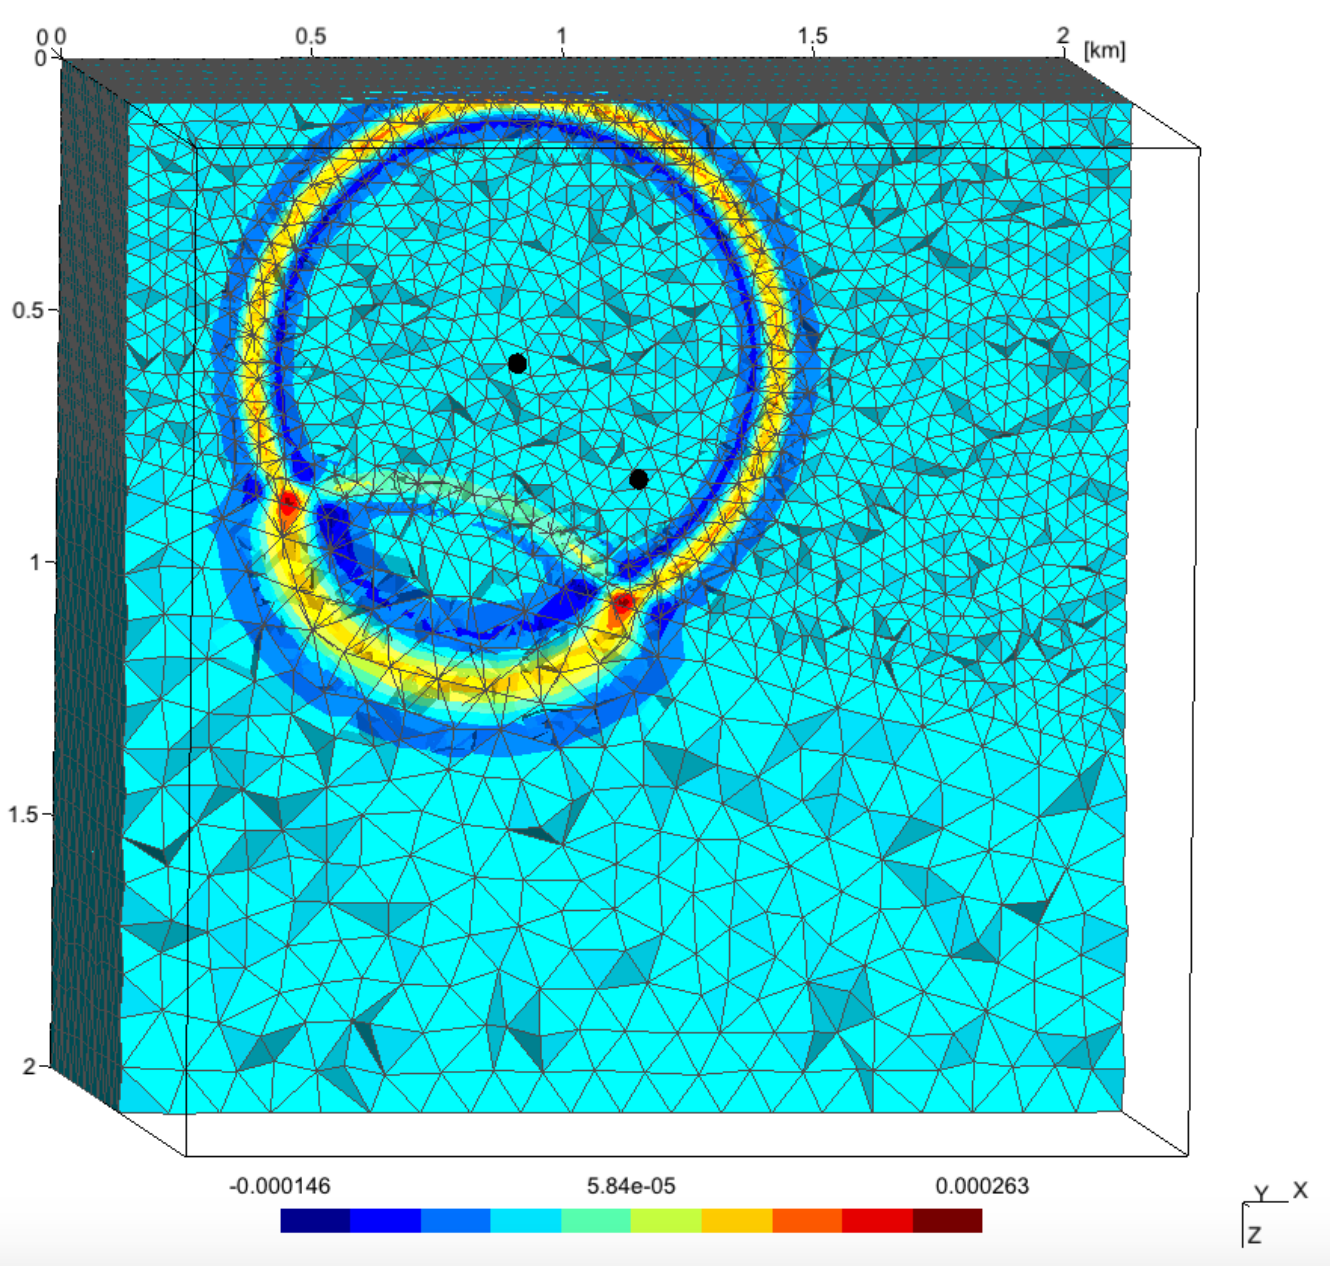
\includegraphics[width=.95\textwidth]{figs/wave.png}
\caption*{Figure courtesy of Axel Modave.}
}
\only<2>{
\includegraphics[width=.95\textwidth]{figs/wave_N1.eps}
\caption*{\textbf{Fine} linear approximation.}
}
\only<3>{
\includegraphics[width=.95\textwidth]{figs/wave_N2.eps}
\caption*{\textbf{Coarse} quadratic approximation.}
}
\only<4>{
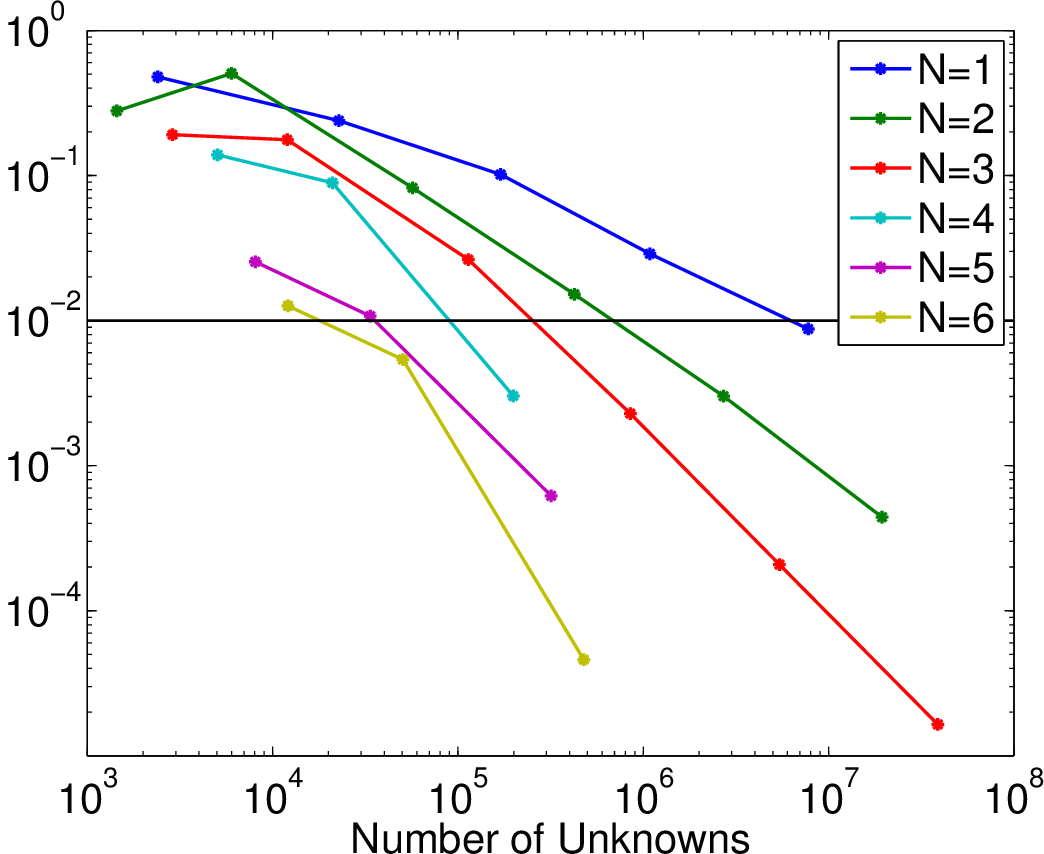
\includegraphics[width=.95\textwidth]{figs/error_v_dofs.png}
\caption*{Max errors vs.\ dofs.}
}
\only<5>{
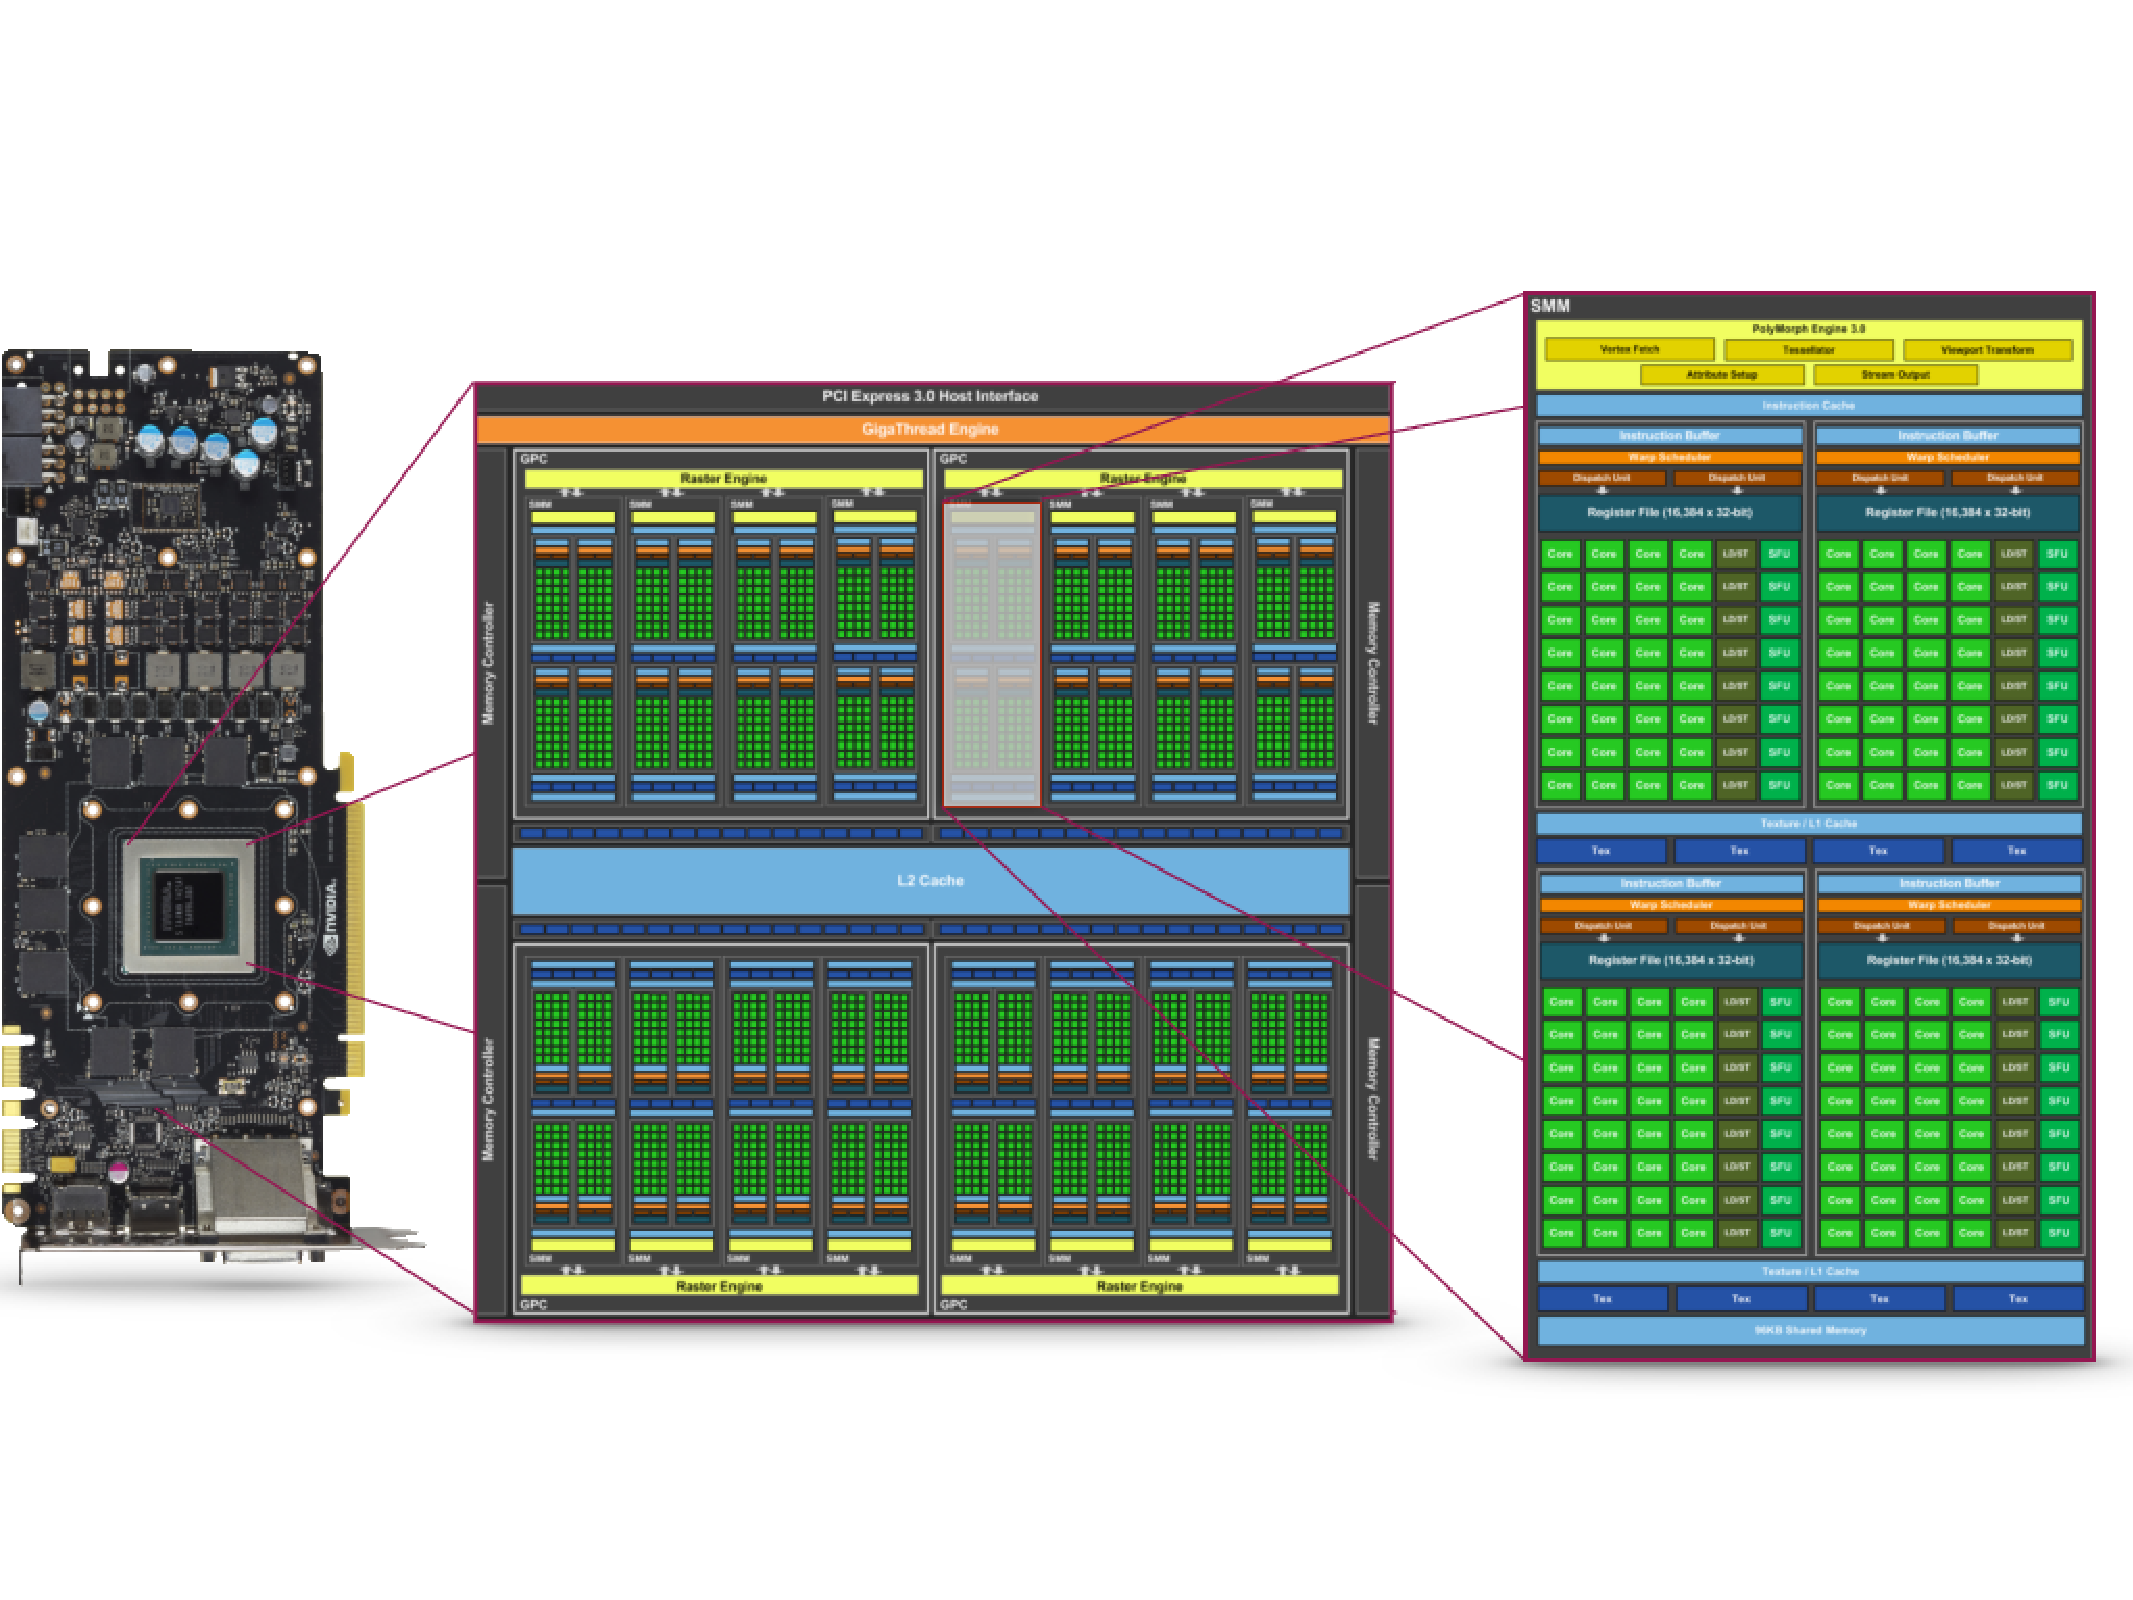
\includegraphics[width=.975\textwidth]{figs/gpu.pdf}
\caption*{Graphics processing units (GPU).}
}
%\caption*{Image courtesy of Axel Modave.}
\end{overlayarea}
\end{figure}
\end{column}
\end{columns}

}


%\frame{
%\frametitle{High order approximation of media and geometry}
%\begin{itemize}
%\item $c^2(\bm{x})$ often assumed piecewise constant for efficiency.
%\vspace{.5em}
%\item Discontinuities in $c^2(\bm{x})$ can result in spurious reflections.
%\vspace{.5em}
%\item Analogous problems with planar approximation of curved geometry.
%\end{itemize}
%
%\begin{figure}
%\subfloat[Mesh and exact $c^2$]{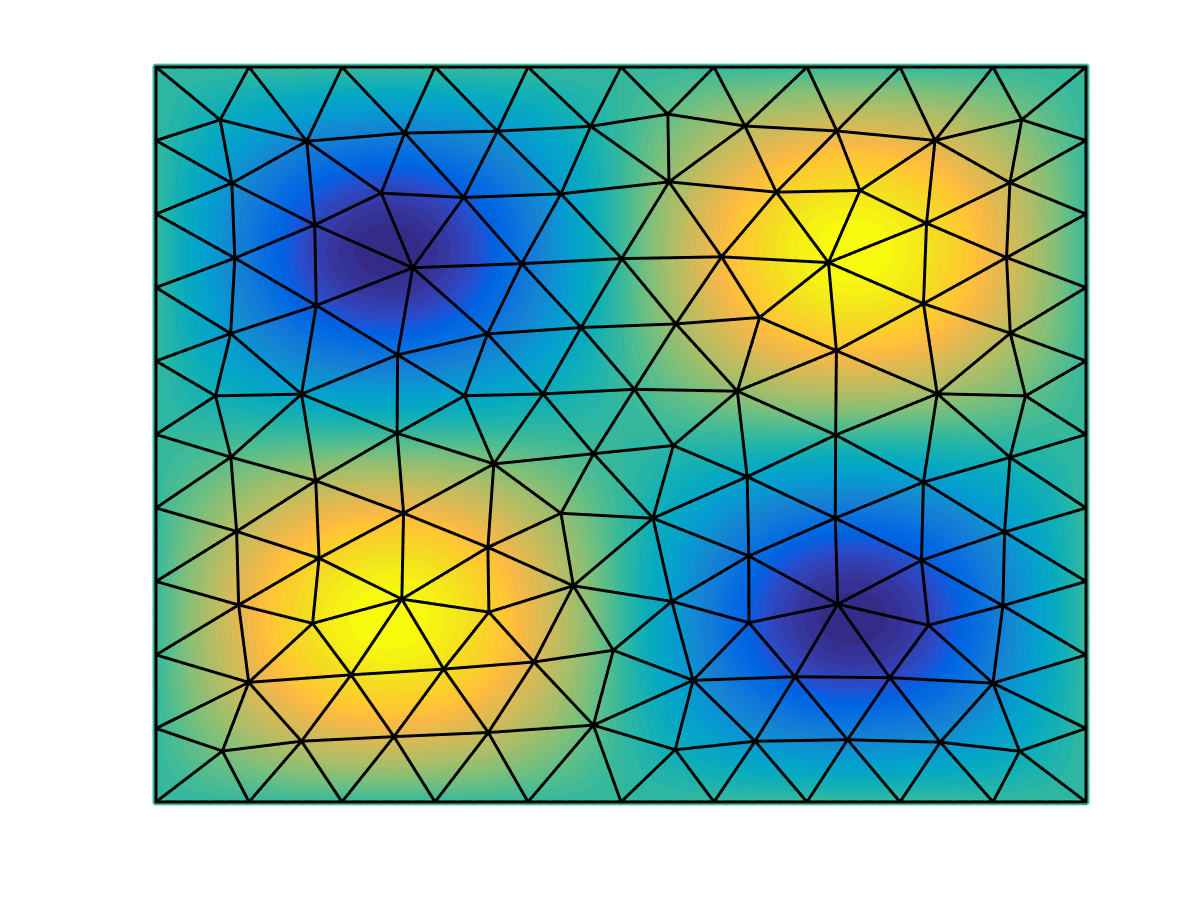
\includegraphics[width=.31\textwidth]{figs/c2WADG.png}}
%\hspace{.2em}
%\subfloat[Piecewise constant $c^2$]{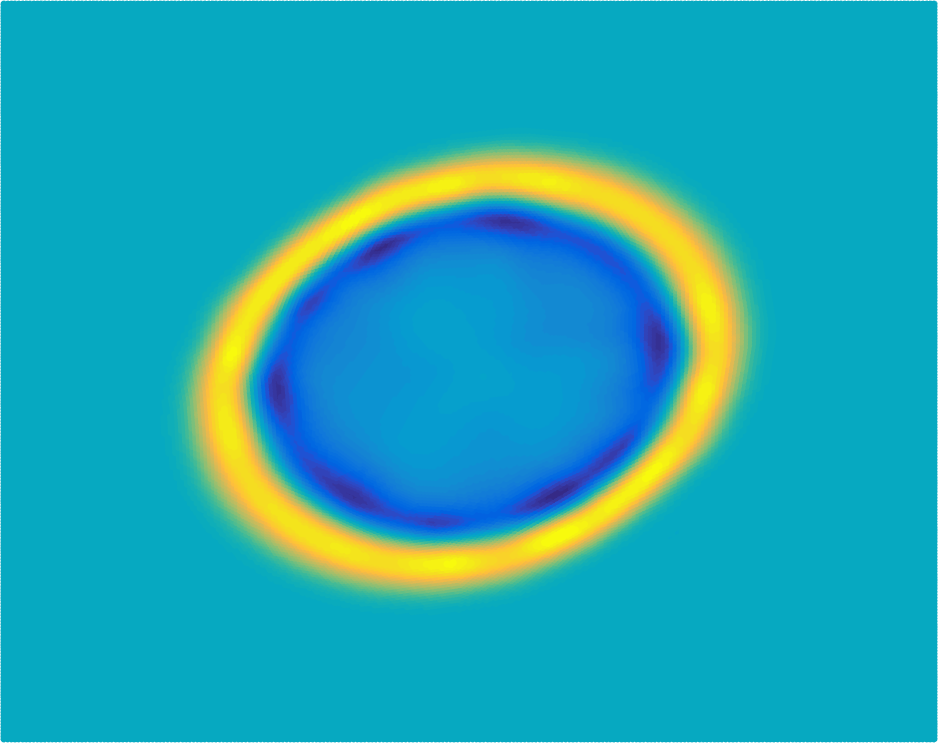
\includegraphics[width=.31\textwidth]{figs/p0WADG.png}}
%\hspace{.2em}
%\subfloat[High order $c^2$]{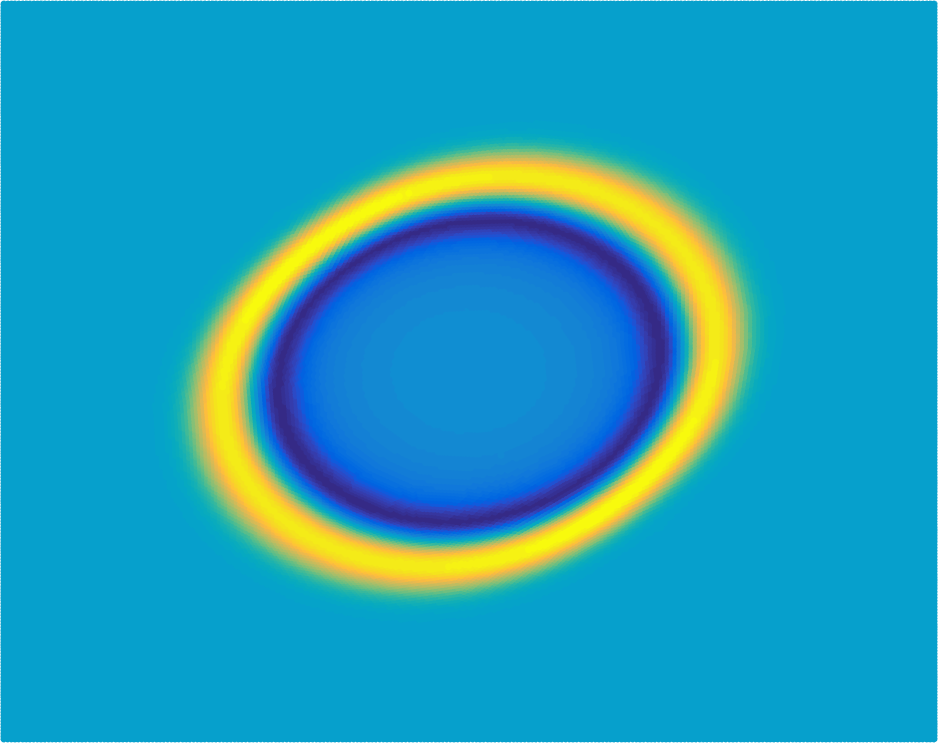
\includegraphics[width=.31\textwidth]{figs/pNWADG.png}}
%\end{figure}
%
%}

\section{Weight-adjusted DG methods: acoustics}

\begin{frame}[noframenumbering]
  \frametitle{Outline}
\only<1>{
 \tableofcontents
}
\only<2>{
 \tableofcontents[currentsection]
}
\end{frame}


\frame{
\frametitle{High order methods and arbitrary heterogeneous media}
\setcounter{subfigure}{0}
\vspace{-1.5em}
\begin{figure}
\subfloat[Mesh and exact $c^2$]{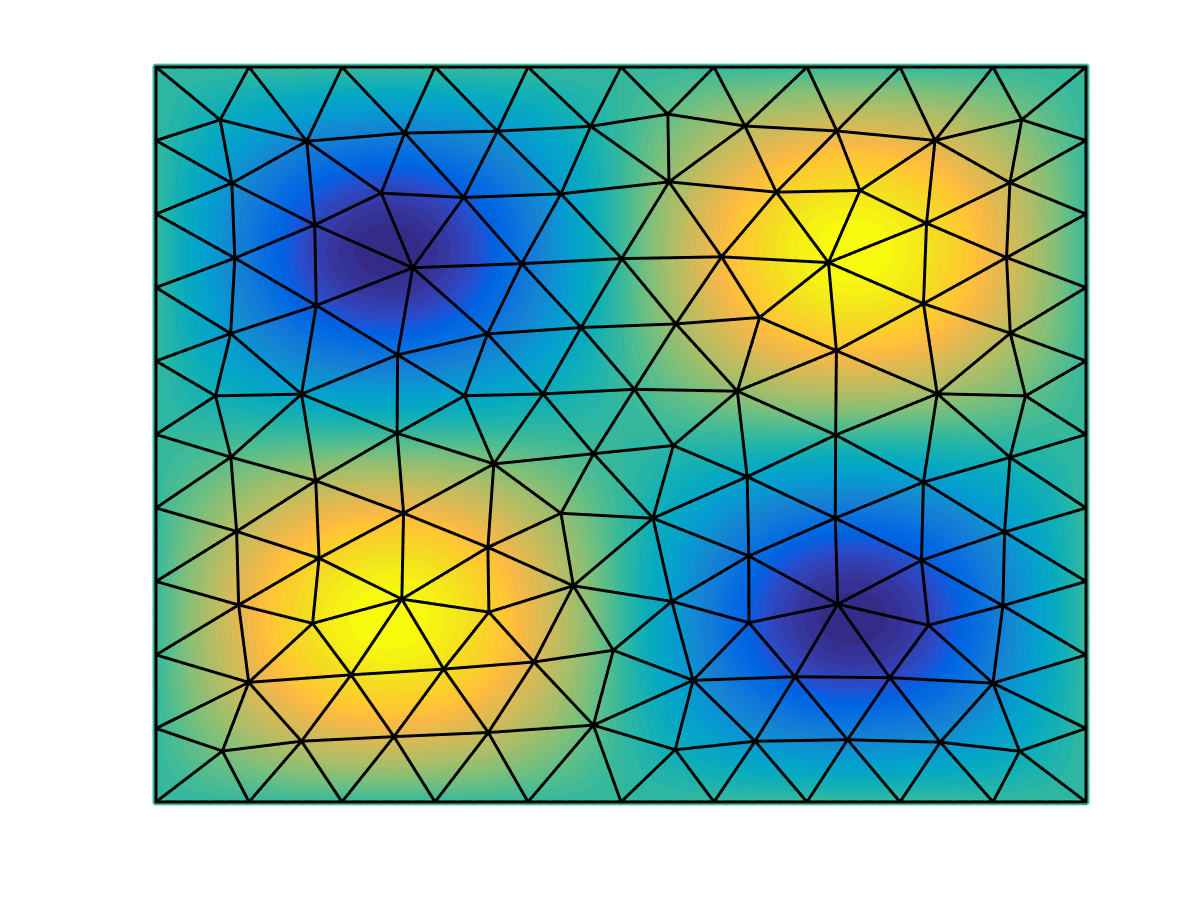
\includegraphics[width=.34\textwidth]{figs/c2WADG.png}}
%\hspace{.1em}
\subfloat[Piecewise const.\ $c^2$]{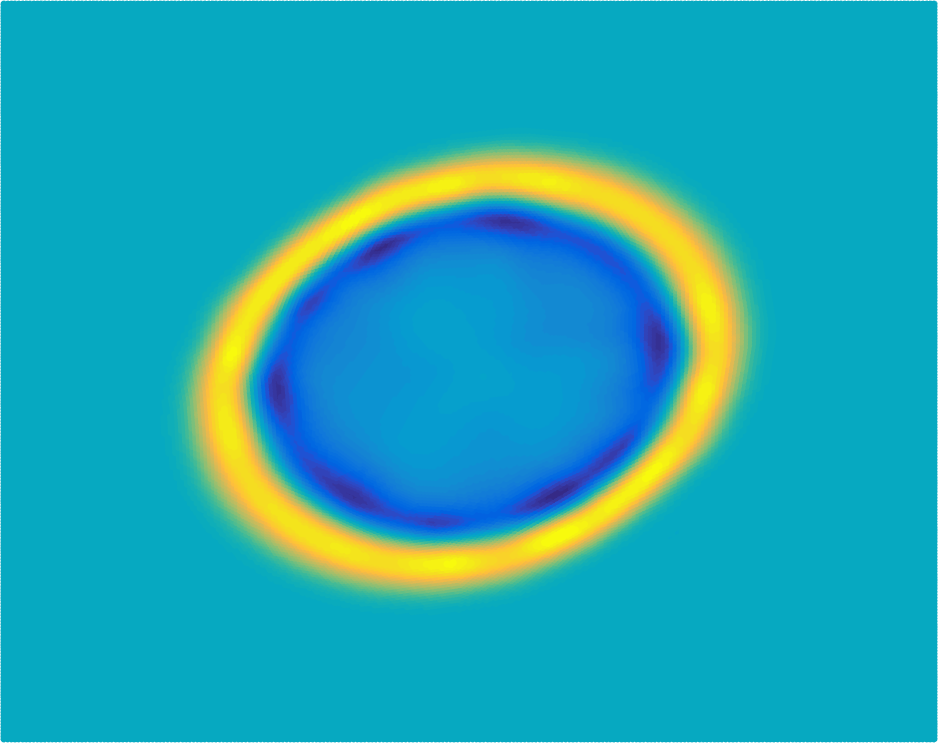
\includegraphics[width=.3\textwidth]{figs/p0WADG.png}}
\hspace{.25em}
\subfloat[High order $c^2$]{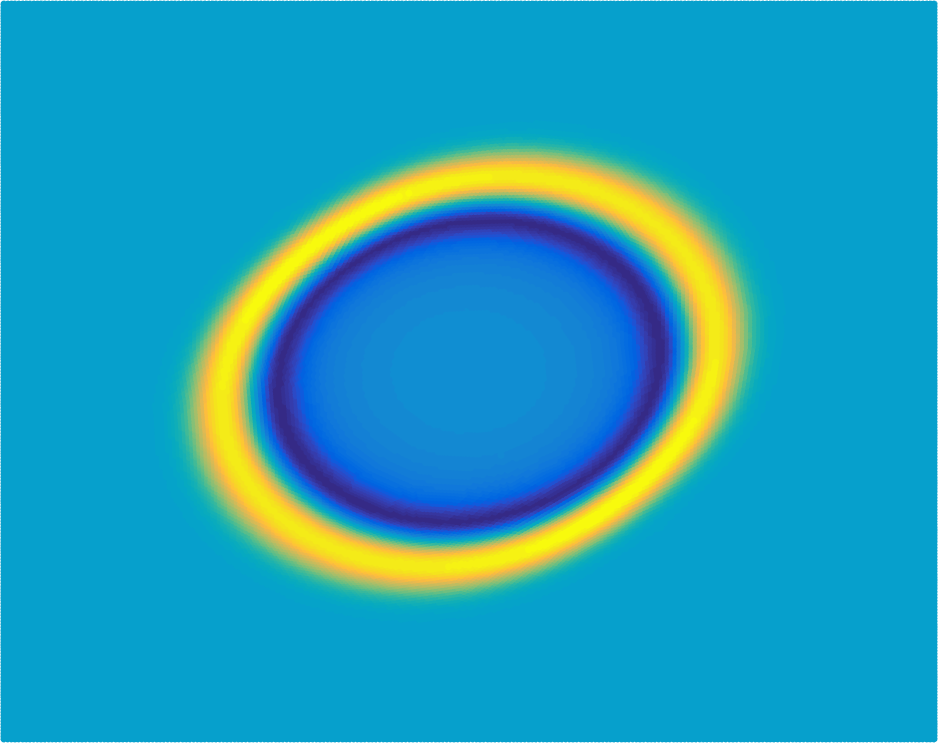
\includegraphics[width=.3\textwidth]{figs/pNWADG.png}}
\end{figure}
\vspace{.5em}
\begin{itemize}
\item Efficient implementations on \textbf{triangular} or \textbf{tetrahedral} meshes assume piecewise constant wavespeed $c^2$.   
\vspace{.25em}
\item High order vs constant approx.\ of media: spurious reflections.  
\vspace{.25em}
\item This talk: generalized mass lumping for DG with provable stability, high order accuracy, simple numerical fluxes (central flux + penalty).
\end{itemize}
}

\frame{
\frametitle{Energy stable discontinuous Galerkin formulations}

\begin{itemize}
\item Model problem: acoustic wave equation (pressure-velocity system)
\begin{align*}
\frac{1}{c^2(\bm{x})}\pd{p}{t}{} = \Div \bm{u}, \qquad \pd{\bm{u}}{t}{} = \Grad p
\end{align*}
\item Local formulation on element $D^k$
\begin{align*}
\int_{D^k}\frac{1}{c^2(\bm{x})}\pd{p}{t}{} q &= \int_{D^k} \Div \bm{u} q  + \frac{1}{2}\int_{\partial D^k} \LRp{\jump{\bm{u}}\cdot{\bm{n}} + \tau_p\jump{p}} q\\
\int_{D^k}\pd{\bm{u}}{t}{} \bm{v} &= \int_{D^k} \Grad p \cdot \bm{v} + \frac{1}{2}\int_{\partial D^k} \LRp{\jump{p} + \tau_u\jump{\bm{u}}\cdot\bm{n}} \bm{v}
\end{align*}
\item Energy stability (penalty terms weakly enforce continuity conditions)
\[
\pd{}{t}{}\LRp{\sum_{k} \int_{D^k} \frac{p^2}{c^2(\bm{x})} + \LRb{\bm{u}}^2} = -\sum_k\int_{\partial D^k} \tau_p\jump{p}^2 +  \tau_u\jump{\bm{u}\cdot\bm{n}}^2 \leq 0.
\]
\end{itemize}
}


\frame{
\frametitle{Semi-discrete formulation and weighted mass matrices}

\begin{itemize}
\item Weighted mass matrix $\bm{M}_{1/c^2}$: SPD, induces weighted norm on $\bm{p}$
\[
\LRp{\bm{M}_{1/c^2}}_{ij} = \int_{D^k} \frac{1}{c^2\LRp{\bm{x}}}\phi_j(\bm{x})\phi_i(\bm{x}) \diff{\bm{x}}.
\]
\item Semi-discrete form: face mass and weak derivative matrices $\bm{M}_f$, $\bm{S}_i$.
\begin{align*}
\bm{M}_{1/c^2} \td{\bm{p}}{t} &= \sum_{i=1}^{d}\bm{S}_i \bm{u}_i + \sum_{\text{faces}} \bm{M}^f \bm{F}_p,\\[1ex]
\bm{M} \td{\bm{u}_i}{t} &= \bm{S}_i \bm{p} +\sum_{\text{faces}}\bm{M}^f\bm{F}_u.
\end{align*}
\item Must build and factorize $\bm{M}_{1/c^2}$ separately over each element (unless $c^2$ constant and $\LRp{\bm{M}_{1/c^2}}^{-1} = c^2\bm{M}^{-1}$).  
\end{itemize}
}


\frame{
\frametitle{Weight-adjusted DG: generalized mass lumping}
\begin{itemize}
\item \textcolor{red}{Weight-adjusted DG (WADG)}: ${\bm{M}} \LRp{{\bm{M}}_{1/w}}^{-1} {\bm{M}}$ is SPD and an energy stable approximation of weighted mass matrix.
\[
\bm{M}_{w}\td{\bm{U}}{t} \approx \textcolor{red}{{\bm{M}} \LRp{{\bm{M}}_{1/w}}^{-1} {\bm{M}}} \td{\bm{U}}{t} = \text{right hand side}.
\]
%\vspace{.1em}
\item Bypasses inverse of weighted matrix $\LRp{\bm{M}_{w}}^{-1}$ 
\[
\LRp{{\bm{M}} \LRp{{\bm{M}}_{1/w}}^{-1}{\bm{M}}}^{-1} = {\bm{M}}^{-1} {{\bm{M}}}_{1/w} {\bm{M}}^{-1}.
\]
%\item Operator evaluation reuses un-weighted implementation
%\begin{align*}
%\only<1>{{\bm{M}} \LRp{{\bm{M}}_{1/w}}^{-1} {\bm{M}} \td{\bm{U}}{t} &= \bm{A}_h \bm{U}}
%\only<2>{\LRp{{\bm{M}}_{1/w}}^{-1} {\bm{M}} \td{\bm{U}}{t} &= \underbrace{\bm{M}^{-1}\bm{A}_h \bm{U} }_{\text{unweighted RHS}}}
%\end{align*}
%\vspace{.1em}
\item Low storage matrix-free application of $\bm{M}^{-1}{\bm{M}}_{1/w}$ using quadrature.
\begin{gather*}
\bm{M} = \bm{V}_q^T\bm{W}\bm{V}_q, \quad \bm{V}_q = \text{ eval.\ at quad.\ pts}, \quad \bm{W} = \text{ quad.\ weights}\\
\LRp{\bm{M}}^{-1} {\bm{M}}_{1/w}\text{RHS} = \underbrace{\widehat{\bm{M}}^{-1} \bm{V}_q^T \bm{W}}_{\bm{P}_q} {\rm diag}\LRp{1/w} \bm{V}_q \LRp{\text{RHS}}.
\end{gather*}
\end{itemize}
}

\frame{
\frametitle{WADG and high order accuracy}
\begin{itemize}
\item Generates norm with same equivalence constants
\[
\only<1>{
w_{\min} \bm{u}^T\bm{M}\bm{u} \leq \bm{u}^T\bm{M}_{w}\bm{u} \leq w_{\max} \bm{u}^T\bm{M}\bm{u} 
}
\only<2->{
w_{\min} \bm{u}^T\bm{M}\bm{u} \leq \bm{u}^T\bm{M}^{-1}\bm{M}_{1/w}\bm{M}^{-1}\bm{u} \leq w_{\max} \bm{u}^T\bm{M}\bm{u} 
}
\]
\item<3-> High order accuracy of weighted projection $P_w$, WADG projection $\tilde{P}_w$ 
\begin{align*}
&\nor{u - \tilde{P}_w u}_{L^2} \leq C_w h^{N+1}  \nor{w}_{W^{N+1,\infty}} \nor{u}_{W^{N+1,2}}\\
&\nor{P_w u - \tilde{P}_w u}_{L^2} \leq C_{w,N} h^{\note{N+2}}  \nor{w}_{W^{N+1,\infty}} \nor{u}_{W^{N+1,2}}.\end{align*}
\item<4-> WADG retains high order accuracy for moments: if $v\in P^M$
\begin{align*}
\LRb{\bm{v}^T\bm{M}_w\bm{u} - \bm{v}^T\bm{M}^{-1}\bm{M}_{1/w}\bm{M}^{-1}\bm{u}} &\leq \\
C_{w} \nor{w}_{W^{N+1,\infty}} &h^{2N+2-M}\nor{u}_{W^{N+1,2}} \nor{v}_{L^2}.
\end{align*}
\end{itemize}
}

%\frame{
%\frametitle{A non-intrusive and low-storage implementation}
%\begin{itemize}
%\item Operator evaluation reuses implementation for $w=1$
%\begin{align*}
%{\bm{M}} \LRp{{\bm{M}}_{1/w}}^{-1} {\bm{M}} \td{\bm{U}}{t} &= \bm{A}_h \bm{U} \\
%\rightarrow \LRp{{\bm{M}}_{1/w}}^{-1} {\bm{M}} \td{\bm{U}}{t} &= \underbrace{\bm{M}^{-1}\bm{A}_h \bm{U} }_{\text{RHS for }w = 1}
%\end{align*}
%%\vspace{.25em}
%\item Low storage: matrix-free application of $\bm{M}^{-1}{\bm{M}}_{1/w}$.  
%\[
%\LRp{\bm{M}}^{-1} {\bm{M}}_{1/w}\text{RHS} = \underbrace{\widehat{\bm{M}}^{-1} \bm{V}_q^T W}_{\bm{P}_q} {\rm diag}\LRp{1/w} \bm{V}_q \LRp{\text{RHS}}.
%\]
%\item Non-intrusive: modify RHS locally before update.  For non-curved meshes, can combine with \textit{optimal complexity} RHS evaluation.\footnotemark
%\end{itemize}
%
%\let\thefootnote\relax\footnotetext{\tiny Chan, Warburton 2015.  {GPU-accelerated Bernstein-Bezier discontinuous Galerkin methods for wave propagation}.}
%}

\frame{
\frametitle{Acoustic wave equation: variable coefficients}
\setcounter{subfigure}{0}
%\vspace{.5em}

\begin{figure}
\centering
\only<1>{
\subfloat[Weight $w = c^2(x,y)$]{
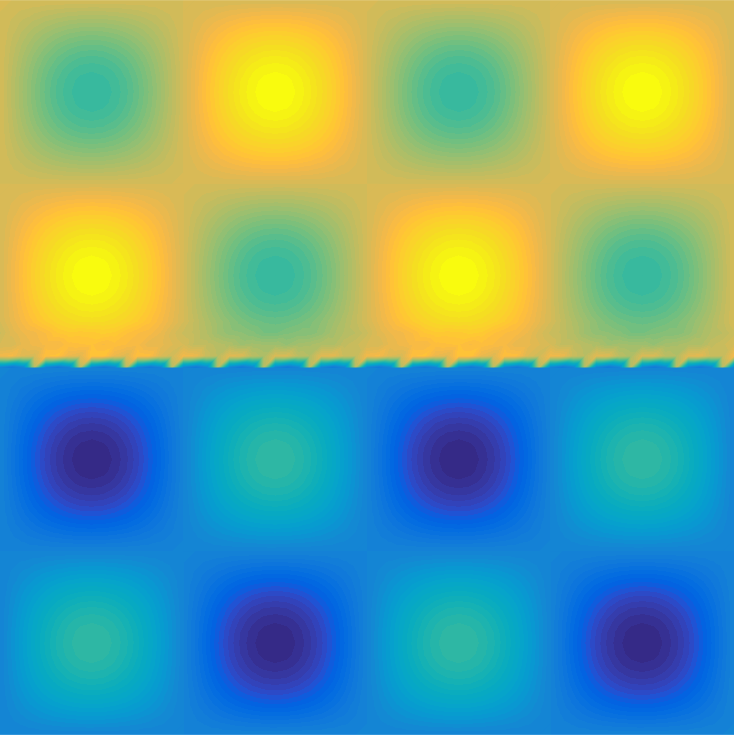
\includegraphics[width=.325\textwidth]{figs/cfun.png}
}
\hspace{1em}
\subfloat[Standard DG]{
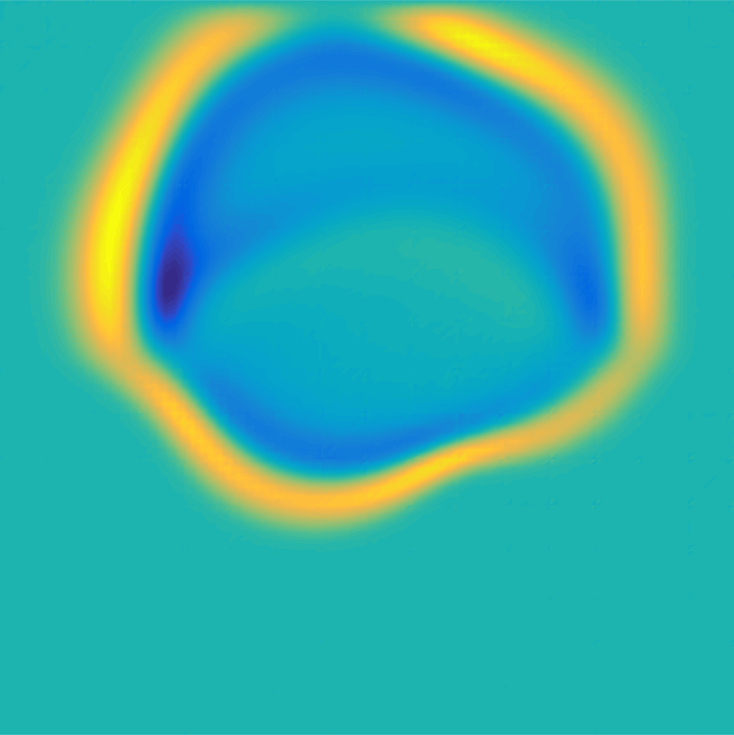
\includegraphics[width=.325\textwidth]{figs/cmass_wave.png}
}}
\only<2>{
\subfloat[Weight $w = c^2(x,y)$]{
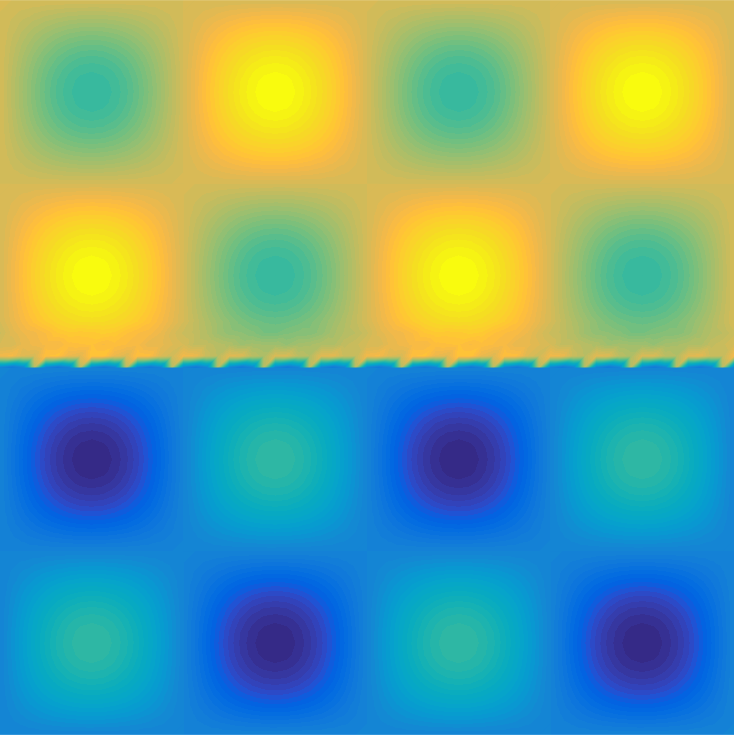
\includegraphics[width=.325\textwidth]{figs/cfun.png}
}
\hspace{1em}
\subfloat[Weighted-adjusted DG]{
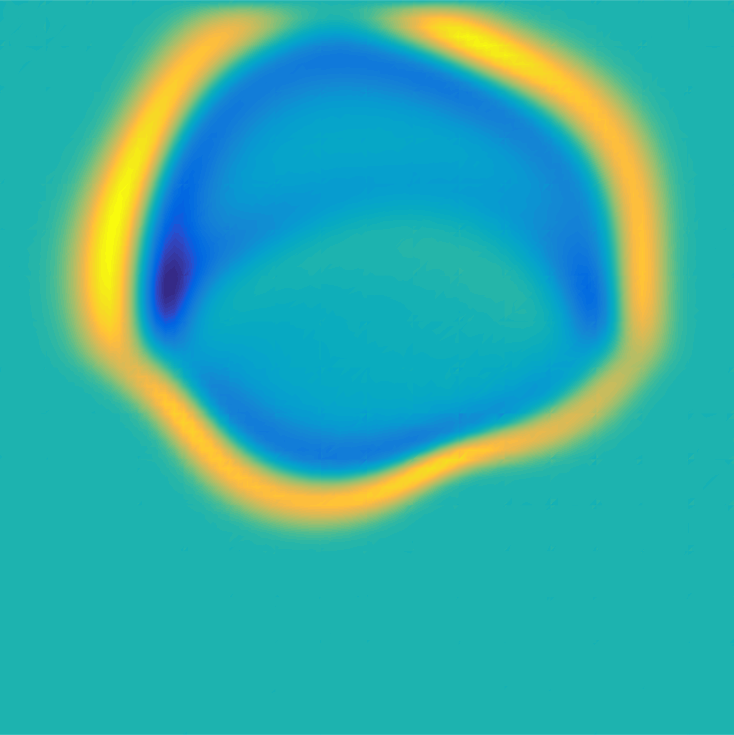
\includegraphics[width=.325\textwidth]{figs/cproj_wave.png}
}}
\caption{Standard vs.\ weight-adjusted DG with spatially varying $c^2$ containing both smooth variations and a discontinuity.}
\end{figure}
%\vspace{.5em}
}


\frame{
\frametitle{Low storage WADG: efficiency on GPUs}

\begin{table}
\centering
\begin{tabular}{|c||c|c|c|c|c|c|c|}
\hline
& $N = 1$ & $N = 2$ & $N = 3$ & $N = 4$ & $N = 5$ & $N = 6$ & $N = 7$\\
\hline
$\bm{M}_{w}^{-1}$ & .66 & 2.79 & 9.90 &29.4 & 73.9 & 170.5 & 329.4\\
\hline
%WADG & .58 & 1.96 & 6.79 & 22.2 & 56.4 & 129.9 &393\\
WADG & 0.59 &   1.44   & 4.30 &   13.9 &   43.0 & 107.8 &  227.7\\
\hline
Speedup &  1.11 &    1.94 &    2.30 &    2.16 &    1.72 &   1.58 &    1.45\\
\hline
\end{tabular}
\caption*{Time (ns) per element: storing/applying $\bm{M}^{-1}_{1/w}$ vs WADG (deg.\ $2N$ quadrature).}
\end{table}

\begin{itemize}
\item Efficiency on GPUs: reduce memory accesses and data movement.
\vspace{.5em}
\item (Tuned) low storage WADG faster than storing and applying $\bm{M}^{-1}_{1/w}$!
\end{itemize}
}

\section{Extension to elastic wave propagation}

\begin{frame}[noframenumbering]
    \frametitle{Outline}
    \tableofcontents[currentsection]
\end{frame}

\frame{
\frametitle{Matrix-valued weights and elastic wave propagation}
\begin{itemize}
\item Symmetric hyperbolic system:  velocity $\bm{v}$, stress $\bm{\sigma}= {\rm vec}(\bm{S})$ with $\bm{\sigma} = \LRp{\sigma_{xx},\sigma_{yy},\sigma_{zz},\sigma_{yz},\sigma_{xz},\sigma_{xy}}^T$.
\begin{align*}
\rho\pd{\bm{v}}{t}{} = \sum_{i=1}^d \bm{A}_i^T \pd{\bm{\sigma}}{\bm{x}_i}{}, \qquad \bm{C}^{-1}\pd{\bm{\sigma}}{t}{} = \sum_{i=1}^d \bm{A}_i \pd{\bm{v}}{\bm{x}_i}{}.
\end{align*}

\item Factoring out the constitutive stiffness tensor $\bm{C}$ results in simple and spatially constant matrices $\bm{A}_i$.  
\[
\bm{C} = \underbrace{\begin{pmatrix}
2\mu + \lambda & \lambda & \lambda &\\
 \lambda & 2\mu + \lambda & \lambda &\\
\lambda & \lambda & 2\mu + \lambda & \\
& & & \mu \bm{I}_{3\times 3}
\end{pmatrix}}_{\text{for isotropic media}}
, \quad
\bm{A}_1 = \left(\begin{array}{ccc}
1 & 0 & 0\\
0 & 0& 0\\
0 & 0& 0\\
0 & 0& 0\\
0 & 0 & 1\\
0 & 1 & 0
\end{array}\right).
%\quad 
%\bm{A}_2 = \left(\begin{array}{ccc}
%0 & 0 & 0\\
%0 & 1 & 0\\
%0 & 0 & 0\\
%0 & 0 & 1\\
%0 & 0 & 0\\
%1 & 0 & 0
%\end{array}\right), \quad
%\bm{A}_3 = \left(\begin{array}{ccc}
%0 & 0 & 0\\
%0 & 0 & 0\\
%0 & 0 & 1\\
%0 & 1 & 0\\
%1 & 0 & 0\\
%0 & 0 & 0
%\end{array}\right)
\]
\end{itemize}
\let\thefootnote\relax\footnotetext{\tiny Hughes and Marsden 1978. Classical elastodynamics as a linear symmetric hyperbolic system.}
}

%\frame{
%\frametitle{Convergence analysis}
%\begin{itemize}
%\item General linear symmetric hyperbolic system
%\[
%\bm{A}_0\pd{\bm{q}}{t}{} = \sum_{j=1}^d \bm{A}_j \pd{\bm{q}}{\bm{x}_i}{}, \qquad  \bm{A}_0 \text{ SPD}, \qquad \bm{A}_i = \bm{A}_i^T.
%\]
%\item General DG formulation: energy stable if $\bm{A}_i$ constant.
%\begin{align*}
%\int_{D^k}\bm{A}_0\pd{\bm{q}}{t}{} \bm{v} =& \int_{D^k}{\sum_{j=1}^d \bm{A}_j \pd{\bm{q}}{\bm{x}_i}{}}\bm{v} + \frac{1}{2}\int_{\partial D^k} \LRp{\bm{A}_n\jump{\bm{q}} + \tau \bm{A}_n^T\bm{A}_n\jump{\bm{q}}}\bm{v}.
%\end{align*}
%\item  \note{Finish}
%\end{itemize}
%}


\frame{
\frametitle{DG formulation for elasticity: energy stability}
\vspace{-.75em}
\begin{itemize}
\item Analogous to acoustics: numerical fluxes independent of media!
\end{itemize}
\vspace{-1em}
\begin{align*}
&\int_{D^k}\LRp{\bm{C}^{-1}\pd{\bm{\sigma}}{t}{}}^T\bm{q} = \int_{D^k}{\sum_{i=1}^d \bm{A}_i \pd{\bm{v}}{\bm{x}_i}{}\bm{q}} + 
\frac{1}{2}\int_{\partial D^k}\LRp{{\bm{A}_n\jump{\bm{v}} + \tau_\sigma\bm{A}_n\bm{A}_n^T\jump{\bm{\sigma}}}}\bm{q},\\
&\int_{D^k}\LRp{\rho\pd{\bm{v}}{t}{}}^T\bm{w} = \int_{D^k}{\sum_{i=1}^d \bm{A}_i^T \pd{\bm{\sigma}}{\bm{x}_i}{}}\bm{w}  + 
\frac{1}{2}\int_{\partial D^k}{\LRp{\bm{A}_n^T\jump{\bm{\sigma}} + \tau_v\bm{A}_n^T\bm{A}_n\jump{\bm{v}}}\bm{w}}.
\end{align*}
\vspace{-1em}
\begin{itemize}
\item Energy method: take $\bm{q}=\bm{\sigma}$, $\bm{w}=\bm{v}$
\begin{gather*}
\int_{D^k}\LRp{\bm{C}^{-1}\pd{\bm{\sigma}}{t}{}}^T\bm{\sigma}
= \pd{}{t}{} \int_{D^k}\LRp{\bm{\sigma}(\bm{x})^T\bm{C}^{-1}(\bm{x})\bm{\sigma}(\bm{x})}\\
\int_{D^k}\LRp{\bm{\rho}\pd{\bm{v}}{t}{}}^T\bm{v}
= \pd{}{t}{}\int_{D^k} \rho(\bm{x})\LRb{\bm{v}}^2.
\end{gather*}
\end{itemize}


}

\frame{
\frametitle{DG formulation for elasticity: energy stability, cont.}
\begin{itemize}
\item $\bm{A}_i$ constant, integration by parts if quadrature exact for degree $(2N-1)$
\begin{overlayarea}{\textwidth}{.32\textheight}
\vspace{-1.5em}
\begin{gather*}
\only<1>{
\int_{D^k}\sum_{i=1}^d \note{\bm{A}_i \pd{\bm{v}}{\bm{x}_i}{}\cdot \bm{q}} + \frac{1}{2}\int_{\partial D^k}\LRp{{\bm{A}_n\jump{\bm{v}} + \tau_\sigma\bm{A}_n\bm{A}_n^T\jump{\bm{\sigma}}}}\cdot\bm{q},\\
\int_{D^k}{\sum_{i=1}^d \bm{A}_i^T \pd{\bm{\sigma}}{\bm{x}_i}{}}\cdot\bm{w}  + \frac{1}{2}\int_{\partial D^k}{\LRp{\bm{A}_n^T\jump{\bm{\sigma}} + \tau_v\bm{A}_n^T\bm{A}_n\jump{\bm{v}}}\cdot\bm{w}}
}
\only<2>{
\int_{D^k}\sum_{i=1}^d \note{-{\bm{v}}\cdot \bm{A}_i^T\pd{\bm{q}}{\bm{x}_i}{}} + \int_{\partial D^k}\note{\LRp{{\bm{A}_n\avg{\bm{v}} + \frac{\tau_\sigma}{2}\bm{A}_n\bm{A}_n^T\jump{\bm{\sigma}}}}}\cdot\bm{q},\\
\int_{D^k}{\sum_{i=1}^d \bm{A}_i^T \pd{\bm{\sigma}}{\bm{x}_i}{}}\cdot\bm{w}  + \frac{1}{2}\int_{\partial D^k}{\LRp{\bm{A}_n^T\jump{\bm{\sigma}} + \tau_v\bm{A}_n^T\bm{A}_n\jump{\bm{v}}}\cdot\bm{w}}
}
\only<3>{
\int_{D^k}\sum_{i=1}^d \note{-{\bm{v}}\cdot \bm{A}_i^T\pd{\bm{\sigma}}{\bm{x}_i}{}} + \int_{\partial D^k}\note{\LRp{{\bm{A}_n\avg{\bm{v}} + \frac{\tau_\sigma}{2}\bm{A}_n\bm{A}_n^T\jump{\bm{\sigma}}}}}\cdot\bm{\sigma},\\
\int_{D^k}{\sum_{i=1}^d \bm{A}_i^T \pd{\bm{\sigma}}{\bm{x}_i}{}}\cdot\bm{v}  + \frac{1}{2}\int_{\partial D^k}{\LRp{\bm{A}_n^T\jump{\bm{\sigma}} + \tau_v\bm{A}_n^T\bm{A}_n\jump{\bm{v}}}\cdot\bm{v}}
}
\only<4>{
\text{Sum volume terms, which cancel to zero } + \\
\hspace{-1em}\int_{\partial D^k} {\LRp{{\bm{A}_n\avg{\bm{v}} + \frac{\tau_\sigma}{2}\bm{A}_n\bm{A}_n^T\jump{\bm{\sigma}}}}}\cdot\bm{\sigma} + \frac{1}{2}{\LRp{\bm{A}_n^T\jump{\bm{\sigma}} + \tau_v\bm{A}_n^T\bm{A}_n\jump{\bm{v}}}\cdot\bm{v}}
}
\only<5>{
\text{Sum volume terms, which cancel to zero } + \\
\hspace{-1em}\int_{\partial D^k} {\LRp{\note{{\bm{A}_n\avg{\bm{v}}}} + \frac{\tau_\sigma}{2}\bm{A}_n\bm{A}_n^T\jump{\bm{\sigma}}}}\cdot\bm{\sigma} + \frac{1}{2}{\LRp{\note{\bm{A}_n^T\jump{\bm{\sigma}}} + \tau_v\bm{A}_n^T\bm{A}_n\jump{\bm{v}}}\cdot\bm{v}}
}
\only<6>{
\text{Sum over all elements: central flux terms cancel } + \\
\sum_k \int_{\partial D^k} \frac{\tau_\sigma}{2}\bm{A}_n\bm{A}_n^T\jump{\bm{\sigma}} \cdot\bm{\sigma} + \frac{\tau_v}{2}\bm{A}_n^T\bm{A}_n\jump{\bm{v}}\cdot\bm{v}
}
\only<7>{
\text{Sum over all elements: combine penalty flux terms} + \\
\sum_k \int_{\partial D^k} \frac{\tau_\sigma}{2}\bm{A}_n^T\jump{\bm{\sigma}}\cdot \bm{A}_n^T\bm{\sigma} + \frac{\tau_v}{2}\bm{A}_n\jump{\bm{v}}\cdot \bm{A}_n\bm{v}
}
\only<8>{
\text{Sum over all elements: combine penalty flux terms} + \\
\sum_k \int_{\partial D^k} \frac{\tau_\sigma}{2}\bm{A}_n^T\jump{\bm{\sigma}} \cdot\bm{A}_n^T\jump{\bm{\sigma}} + \frac{\tau_v}{2}\bm{A}_n\jump{\bm{v}}\cdot\bm{A}_n\jump{\bm{v}}
}
\only<9->{
\text{Sum over all elements: combine penalty flux terms} + \\
\sum_k \int_{\partial D^k} \frac{\tau_\sigma}{2}\bm{A}_n^T\jump{\bm{\sigma}} \cdot\bm{A}_n^T\jump{\bm{\sigma}} + \frac{\tau_v}{2}\bm{A}_n\jump{\bm{v}}\cdot\bm{A}_n\jump{\bm{v}}\\
\text{\ldots and done!}
}
\end{gather*}
\end{overlayarea}
\item Energy stability (penalty weakly enforces continuity conditions):
\begin{align*}
\sum_{D^k} \frac{1}{2}\pd{}{t}{}&\int_{D^k}{\rho \LRb{\bm{v}}^2  + \bm{\sigma}^T\bm{C}^{-1} \bm{\sigma}} =\\
&- \sum_{\text{faces}} \int_{f}{\frac{\tau_{\bm{v}}}{2}\LRb{\bm{A}_n\jump{\bm{v}}}^2 + \frac{\tau_{\bm{\sigma}}}{2}\LRb{\bm{A}_n^T\jump{\bm{\sigma}}}^2} \leq 0.
\end{align*}
\item $\tau_v, \tau_{\sigma} > 0$ penalizes normal jumps ${\jump{\bm{v}}\cdot\bm{n}} \approx 0$, $\jump{\bm{S}}\cdot\bm{n} \approx 0$.
\end{itemize}
}

\frame{
\frametitle{Semi-discrete system: matrix-valued weighted}
\begin{itemize}
\item Matrix-weighted mass matrix: let $\bm{W}\in \mathbb{R}^{d\times d}$ be SPD with entries $w_{ij}$
\[
{\bm{M}_{\bm{W}}} = \LRp{\begin{array}{ccc}
\bm{M}_{w_{11}} & \ldots & \bm{M}_{w_{1d}}\\
\vdots & \ddots & \vdots\\
\bm{M}_{w_{d1}} & \ldots & \bm{M}_{w_{dd}}\\
\end{array}}
\]
\item Semi-discrete DG formulation involves $\bm{C}^{-1}$-weighted mass matrix
\begin{align*}
\bm{M}_{\bm{C}^{-1}}\frac{\partial\bm{\Sigma}}{\partial t}&=\sum_{i=1}^{d}\left(\bm{A}_i\otimes \bm{S}_i\right)\bm{V}+\sum_{\text{faces}}\left(\bm{I}\otimes\bm{M}^f\right)\bm{F}_\sigma,\\ %\qquad \text{(Stress eq.)}\\
\bm{M}_{\rho\bm{I}}\frac{\partial\bm{V}}{\partial t}&=\sum_{i=1}^{d}\left(\bm{A}_i^T\otimes \bm{S}_i\right)\bm{\Sigma}+\sum_{\text{faces}}\left(\bm{I}\otimes\bm{M}^f\right)\bm{F}_v.
\end{align*}
\end{itemize}
}

\frame{
\frametitle{Weight-adjusted DG: matrix-valued weights}
\vspace{-.5em}
\begin{itemize}
\item Matrix-weighted mass matrix large, hard to invert
\[
{\bm{M}_{\bm{C}^{-1}}} = \LRp{\begin{array}{ccc}
\bm{M}_{\bm{C}^{-1}_{11}} & \ldots & \bm{M}_{\bm{C}^{-1}_{1d}}\\
\vdots & \ddots & \vdots\\
\bm{M}_{\bm{C}^{-1}_{d1}} & \ldots & \bm{M}_{\bm{C}^{-1}_{dd}}\\
\end{array}}
\]
\item Weight-adjusted approximation for $\bm{C}^{-1}$ decouples each component
\[
\bm{M}_{\bm{C}^{-1}}^{-1} \approx \LRp{\bm{I}\otimes \bm{M}^{-1}} \bm{M}_{\bm{C}} \LRp{\bm{I} \otimes\bm{M}^{-1}}.
\]
\item Evaluate RHS components at quadrature points, apply $\bm{C}(\bm{x}_i)$ to component vectors at quadrature points, project back to polynomials.
\vspace{.01em}
\item Recovers Kronecker product $\bm{M}_{\bm{C}^{-1}}^{-1} = \bm{C}\otimes \bm{M}^{-1}$ for constant $\bm{C}^{-1}$.
\end{itemize}
}

\frame{
\frametitle{Energy stability and DG spectra}
\setcounter{subfigure}{0}
\vspace{-2em}
\begin{figure}
\centering
\subfloat[Central flux ($\tau_v, \tau_{\sigma}= 0$)]{
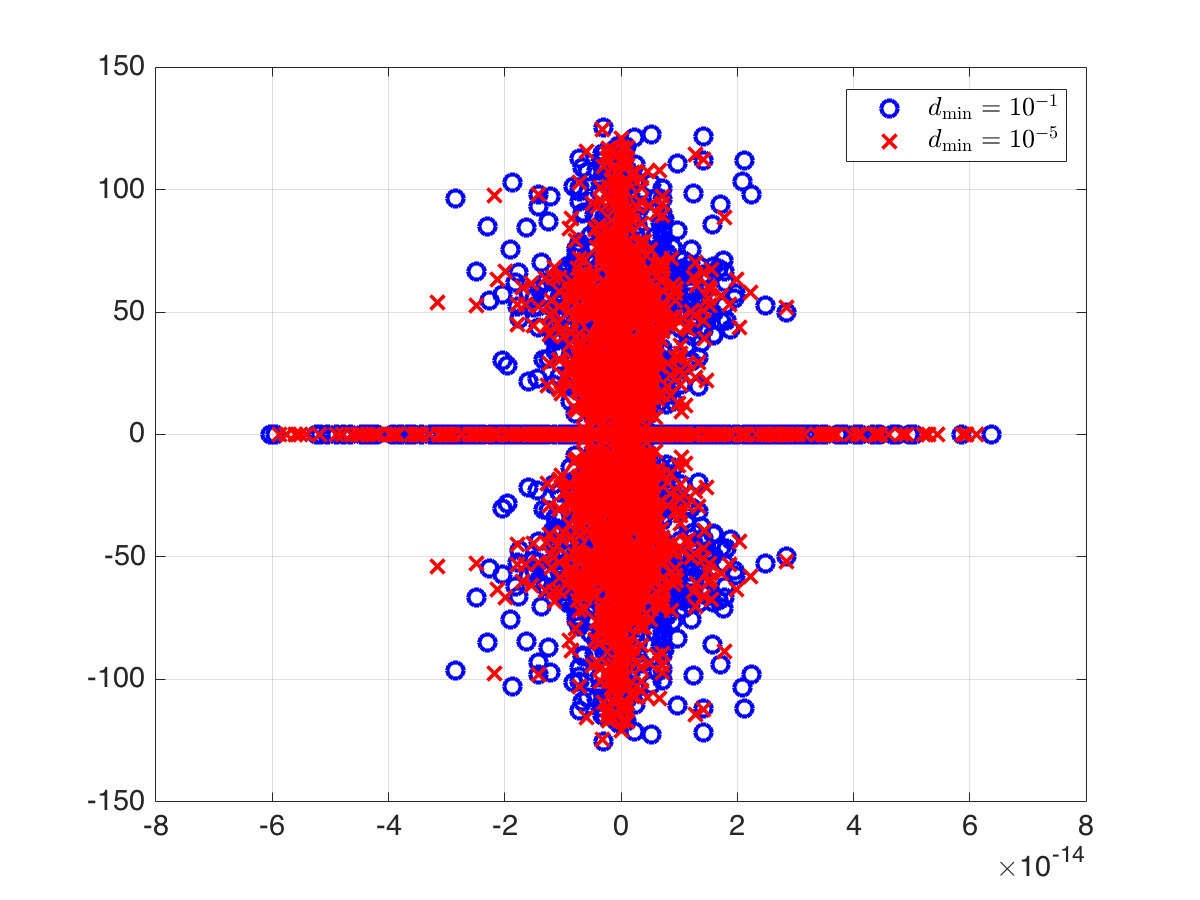
\includegraphics[width=.45\textwidth]{figs/spectra_tau0.png}
}
\subfloat[Penalty flux ($\tau_v, \tau_{\sigma}= 1$)]{
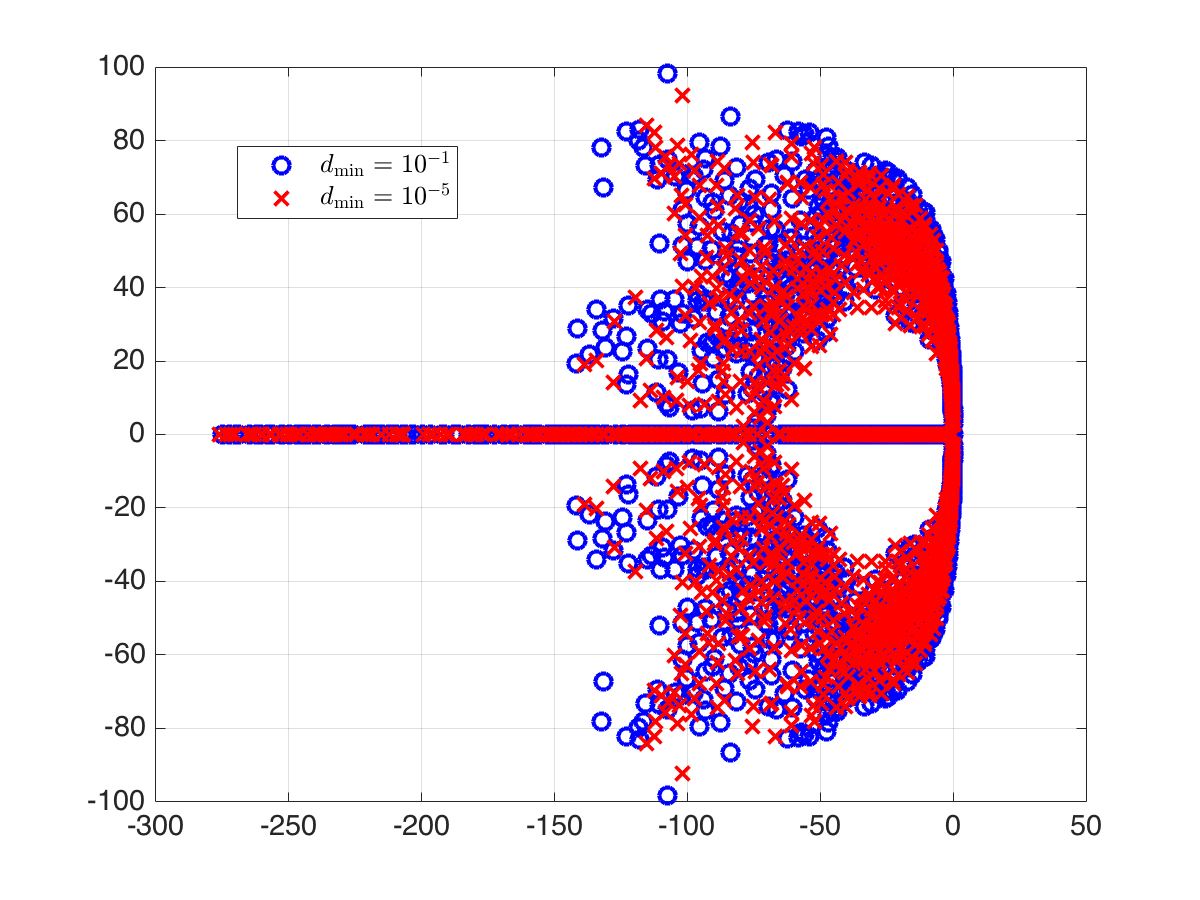
\includegraphics[width=.45\textwidth]{figs/spectra_tau1.png}
}
\caption{DG spectra with random heterogeneities at each quadrature point. }
\end{figure}
\vspace{-.5em}
\begin{itemize}
\item Guaranteed energy stability for both energy conservative and energy dissipative numerical interface fluxes.
\item CFL can be improved by setting $\tau_\sigma \approx 1/\nor{\bm{C}}$, $\tau_v \approx \nor{\rho}$
\end{itemize}
}


\frame{
\frametitle{Elastic wave propagation: convergence}
\setcounter{subfigure}{0}
\begin{itemize}
\item Convergence for harmonic oscillation, Rayleigh, Lamb, and Stoneley waves: between $O(h^{N+1})$ and $O(h^{N+1/2})$.  
\vspace{1em}
\item $\bm{\sigma}$ error grows as $\nor{\bm{C}^{-1}}\rightarrow \infty$ (e.g.\ incompressible limit $\lambda/\mu \rightarrow \infty$).  
\end{itemize}
\vspace{-1em}
\begin{figure}
\centering
\subfloat[$L^2$ errors (Stoneley wave) ]{
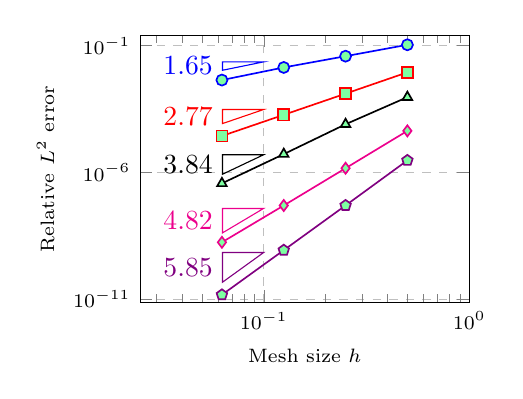
\begin{tikzpicture}
\begin{loglogaxis}[
    legend cell align=left,
    legend style={legend pos=south east, font=\tiny},
    width=.475\textwidth,
    xlabel={Mesh size $h$},
    ylabel={Relative $L^2$ error}, 
    xmin=.025, xmax=1,
    ymin=.75e-11, ymax=.25,
    xmajorgrids=true,
    ymajorgrids=true,
    grid style=dashed,
] 

\addplot[color=blue,mark=*,semithick, mark options={fill=markercolor}]
coordinates{(0.5,0.108456)(0.25,0.0385149)(0.125,0.0138288)(0.0625,0.0043988)};    
\logLogSlopeTriangleFlip{0.375}{0.125}{0.87}{1.65}{blue}

\addplot[color=red,mark=square*,semithick, mark options={fill=markercolor}]
coordinates{(0.5,0.00887301)(0.25,0.00128102)(0.125,0.000186756)(0.0625,2.73376e-05)};    
\logLogSlopeTriangleFlip{0.375}{0.125}{0.67}{2.77}{red}

\addplot[color=black,mark=triangle*,semithick, mark options={fill=markercolor}]
coordinates{(0.5,0.000930299)(0.25,7.92165e-05)(0.125,5.2534e-06)(0.0625,3.67676e-07)};    
\logLogSlopeTriangleFlip{0.375}{0.125}{0.48}{3.84}{black}

\addplot[color=magenta,mark=diamond*,semithick, mark options={fill=markercolor}]
coordinates{(0.5,4.34823e-05)(0.25,1.45784e-06)(0.125,4.92754e-08)(0.0625,1.74105e-09)};   
\logLogSlopeTriangleFlip{0.375}{0.125}{0.26}{4.82}{magenta}

\addplot[color=violet,mark=pentagon*,semithick, mark options={fill=markercolor}]
coordinates{(0.5,2.97005e-06)(0.25,4.94512e-08)(0.125,8.48451e-10)(0.0625,1.47109e-11)};  
\logLogSlopeTriangleFlip{0.375}{0.125}{0.075}{ 5.85}{violet}

%\node at (axis cs:.03,6.8e-10) {$u$ discontinuous};
%\legend{$N=1$,$N=2$,$N=3$,$N=4$,$N=5$}
\end{loglogaxis}
\end{tikzpicture}
}
\subfloat[$\nor{\bm{C^{-1}}}\rightarrow \infty$, $N=3, h = 1/8$.]{
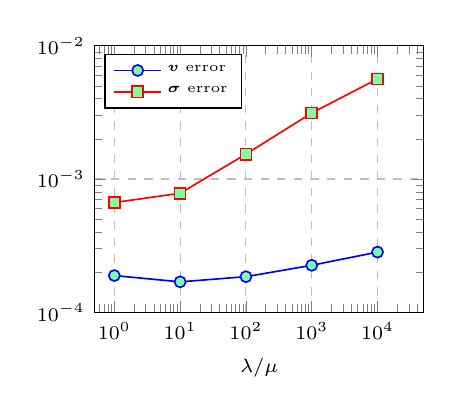
\begin{tikzpicture}
\begin{loglogaxis}[
    legend cell align=left,
    legend style={legend pos=north west, font=\tiny},
    width=.475\textwidth,
    xlabel={$\lambda / \mu$},
%    ylabel={Relative $L^2$ error}, 
    xmin=.5, xmax=5e4,
    ymin=1e-4, ymax=1e-2,
    xmajorgrids=true,
    ymajorgrids=true,
    grid style=dashed,
] 

\addplot[color=blue,mark=*,semithick, mark options={fill=markercolor}]
coordinates{(1,0.00018867)(10,0.00016925)(100,0.00018509)(1000,0.0002252)(10000,0.00028301)};

\addplot[color=red,mark=square*,semithick, mark options={fill=markercolor}]
coordinates{(1,0.00066596)(10,0.00078157)(100,0.0015353)(1000,0.0031239)(10000,0.0056341)};

\legend{$\bm{v}$ error, $\bm{\sigma}$ error }
\end{loglogaxis}
\end{tikzpicture}
}
\end{figure}
%\item Single precision energy stability 
}

\frame{
\frametitle{Elastic wave propagation: stiff inclusion}
\begin{figure}
\centering
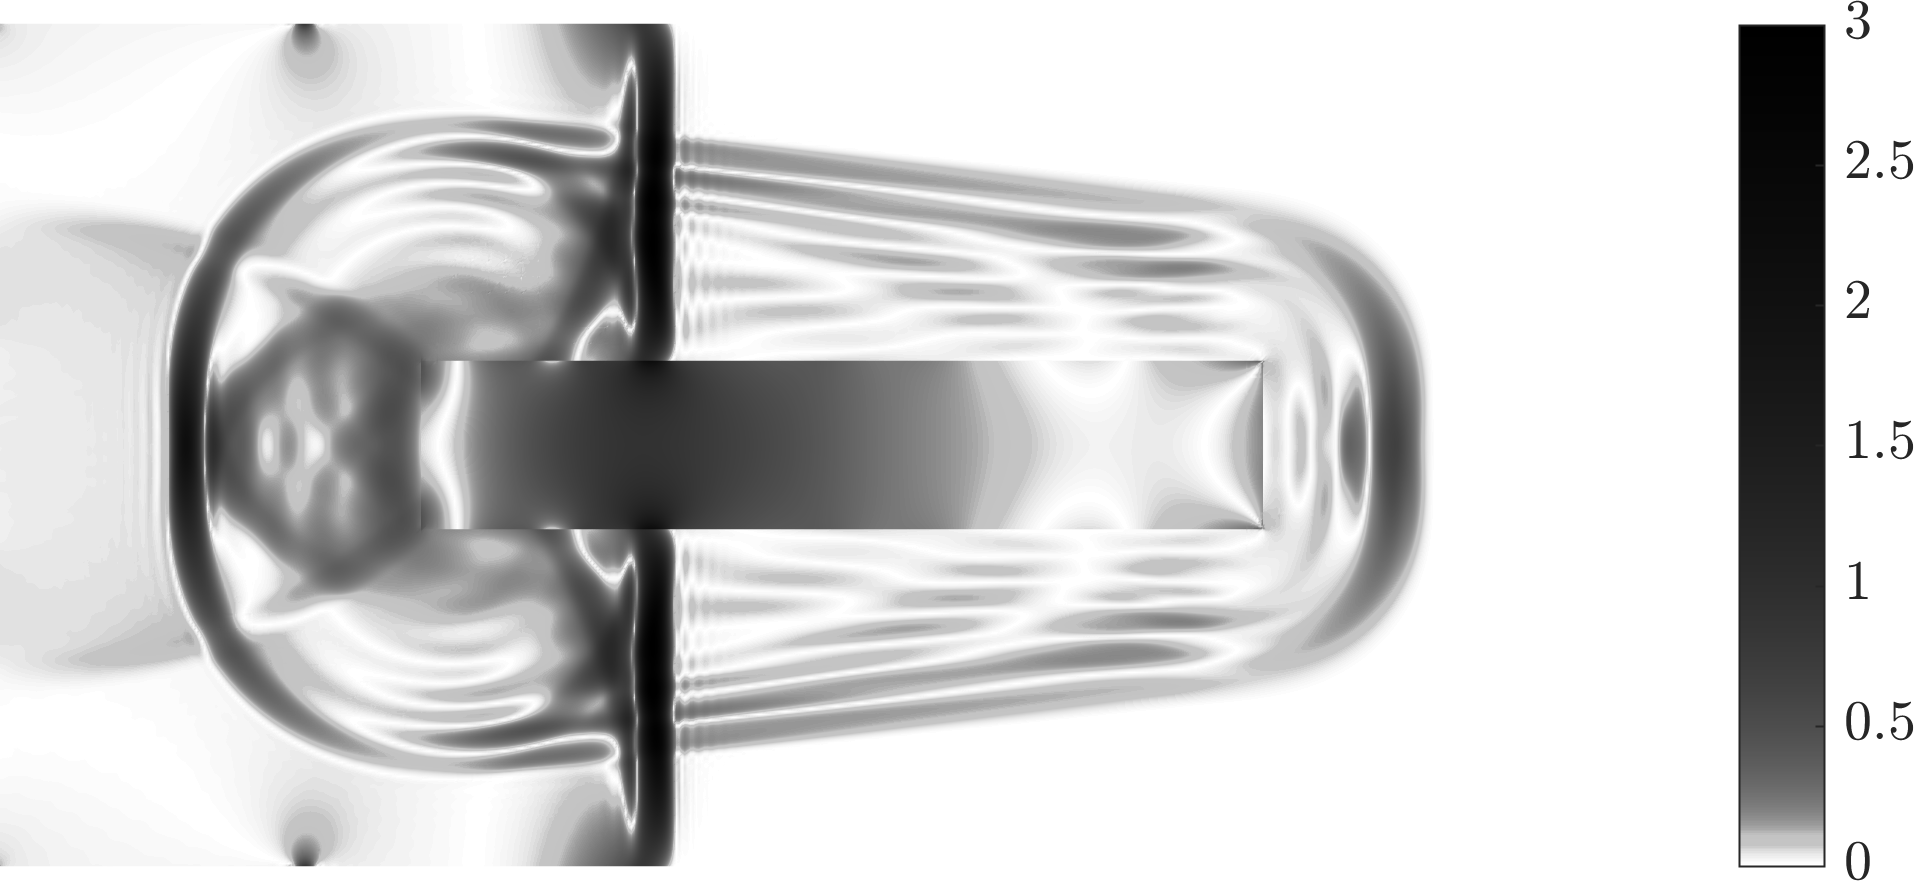
\includegraphics[width=.575\textwidth]{figs/inclusion_aligned.png}\\
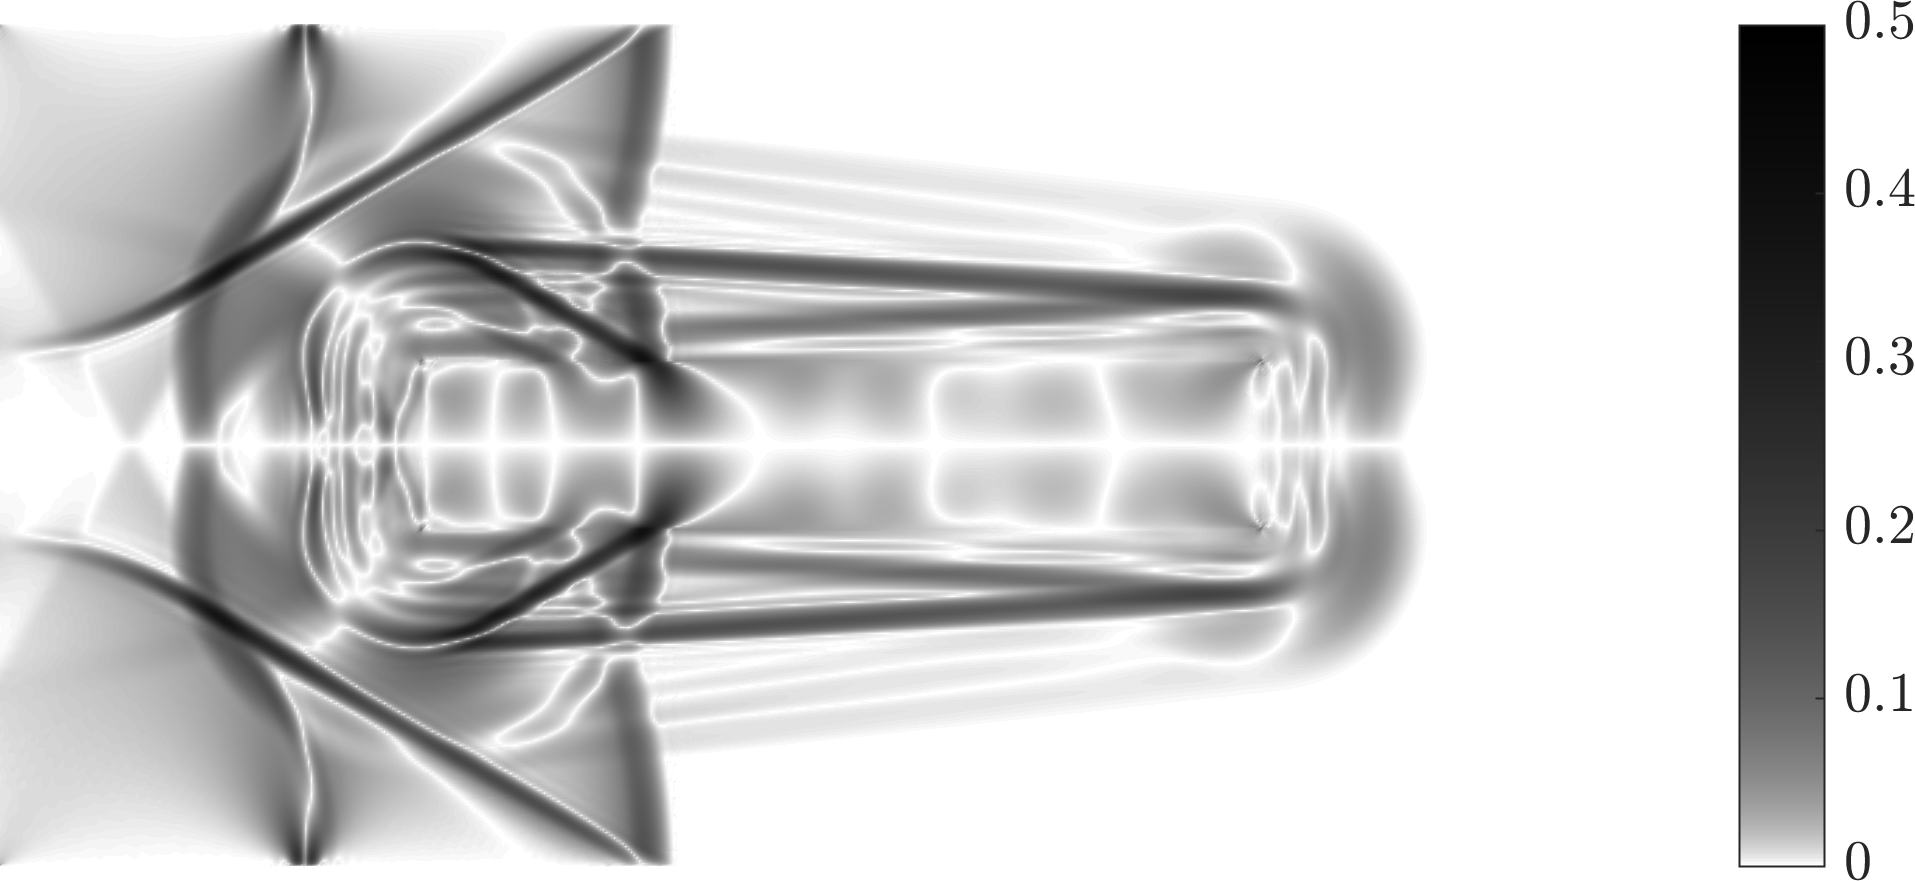
\includegraphics[width=.575\textwidth]{figs/inclusion_aligned_shear.png}
\caption{${\rm tr}(\bm{\sigma})$ and $\bm{\sigma}_{xy}$ for stiff inclusion with $N=5$, $h\approx 1/50$.}
\end{figure}
}

\frame{
\frametitle{Elastic wave propagation: anisotropy}
\setcounter{subfigure}{0}
\vspace{.5em}
Simple implementation for anisotropy - fluxes independent of $\bm{C}$. 
\vspace{-.5em}
\begin{figure}
\centering
\subfloat[Vertical velocity, $t=30\mu s$]{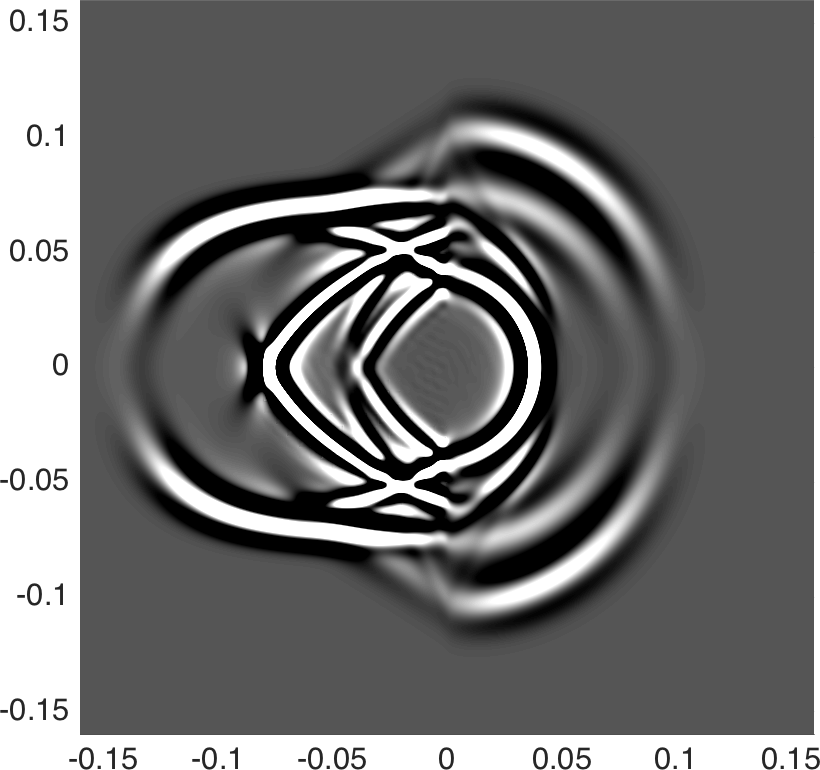
\includegraphics[height=.525\textheight]{figs/aniso1.png}}
\subfloat[Vertical velocity, $t=60 \mu s$]{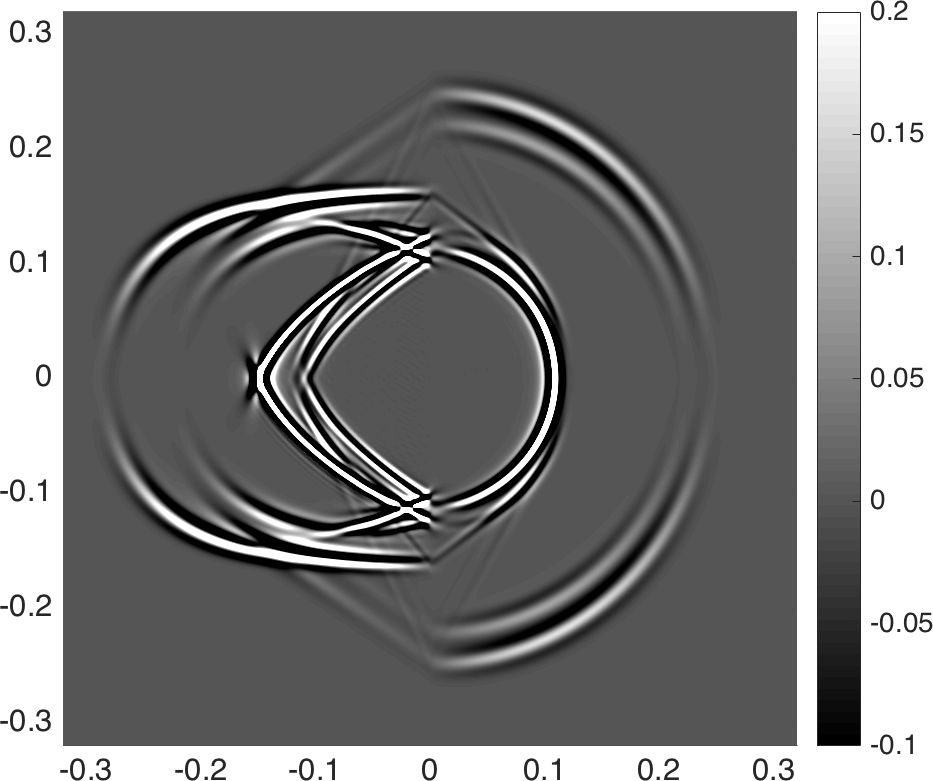
\includegraphics[height=.526\textheight]{figs/aniso2.png}}
\caption*{Anisotropic heterogeneous media: transverse isotropy ($x < 0$), isotropy ($x > 0$).}
\end{figure}

\let\thefootnote\relax\footnotetext{\tiny Komatitsch, Barnes, Tromp 2000. Simulation of anisotropic wave propagation based upon a spectral element method.}
}


\frame{
\frametitle{Curved meshes and heterogeneous media}

%\begin{align*}
%&\int_{D^k}\LRp{\bm{C}^{-1}\pd{\bm{\sigma}}{t}{}}^T\bm{q} = \int_{D^k}{\sum_{i=1}^d \bm{A}_i \pd{\bm{v}}{\bm{x}_i}{}\bm{q}} + 
%\frac{1}{2}\int_{\partial D^k}\LRp{{\bm{A}_n\jump{\bm{v}} + \tau_\sigma\bm{A}_n\bm{A}_n^T\jump{\bm{\sigma}}}}\bm{q},\\
%&\int_{D^k}\LRp{\rho\pd{\bm{v}}{t}{}}^T\bm{w} = \int_{D^k}{\sum_{i=1}^d \bm{A}_i^T \pd{\bm{\sigma}}{\bm{x}_i}{}}\bm{w}  + 
%\frac{1}{2}\int_{\partial D^k}{\LRp{\bm{A}_n^T\jump{\bm{\sigma}} + \tau_v\bm{A}_n^T\bm{A}_n\jump{\bm{v}}}\bm{w}}.
%\end{align*}
\begin{itemize}
\item Map curved elements $D^k$ to reference element $\hat{D}$, introduce determinant of Jacobian of mapping $J$ (varies of $\hat{D}$).
\item RHS terms: discretize skew-symmetric form
\begin{gather*}
 \int_{\hat{D}}{\sum_{i=1}^d -\bm{v}\cdot\bm{A}_i^T\pd{\bm{q}}{\bm{x}_i}{}}J + 
\int_{\partial D^k}\LRp{{\bm{A}_n\avg{\bm{v}} + \frac{\tau_\sigma}{2}\bm{A}_n\bm{A}_n^T\jump{\bm{\sigma}}}}\bm{q},\\
 \int_{\hat{D}}{\sum_{i=1}^d \bm{A}_i^T \pd{\bm{\sigma}}{\bm{x}_i}{}}\cdot\bm{w} J + 
\frac{1}{2}\int_{\partial D^k}{\LRp{\bm{A}_n^T\jump{\bm{\sigma}} + \tau_v\bm{A}_n^T\bm{A}_n\jump{\bm{v}}}\bm{w}}.
\end{gather*}
\item Time-derivative terms: $J$ incorporated into matrix weighting.
\[
\int_{D^k}\LRp{\bm{C}^{-1}\pd{\bm{\sigma}}{t}{}}^T\bm{q} = 
\int_{\hat{D}}\LRp{\note{J\bm{C}^{-1}}\pd{\bm{\sigma}}{t}{}}^T\bm{q}.
\]
%\item \note{FINISH}
\end{itemize}
}

\frame{
\frametitle{Curved meshes and random heterogeneous media}
\setcounter{subfigure}{0}
\vspace{-1em}
\begin{figure}
\centering
\subfloat{
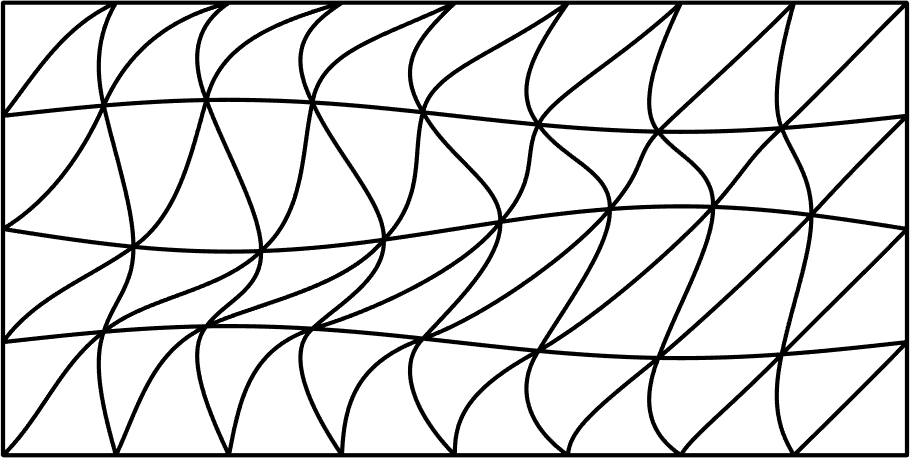
\includegraphics[width=.35\textwidth]{figs/curvedMesh.png}}\\
\vspace{-1em}
\subfloat[Central flux ($\tau_v, \tau_{\sigma} = 0$)]{
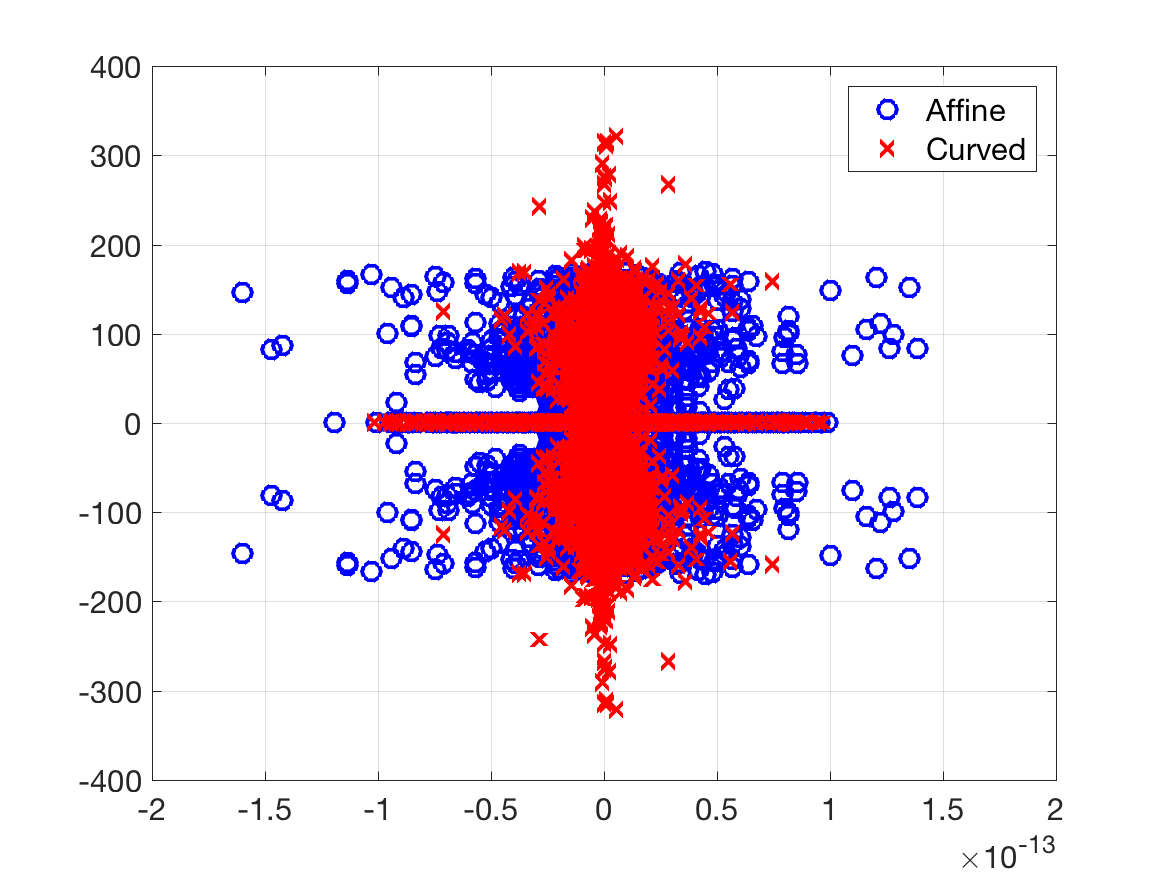
\includegraphics[width=.475\textwidth]{figs/eig_curved_tau0.png}}
\subfloat[Central flux ($\tau_v, \tau_{\sigma} = 1$)]{
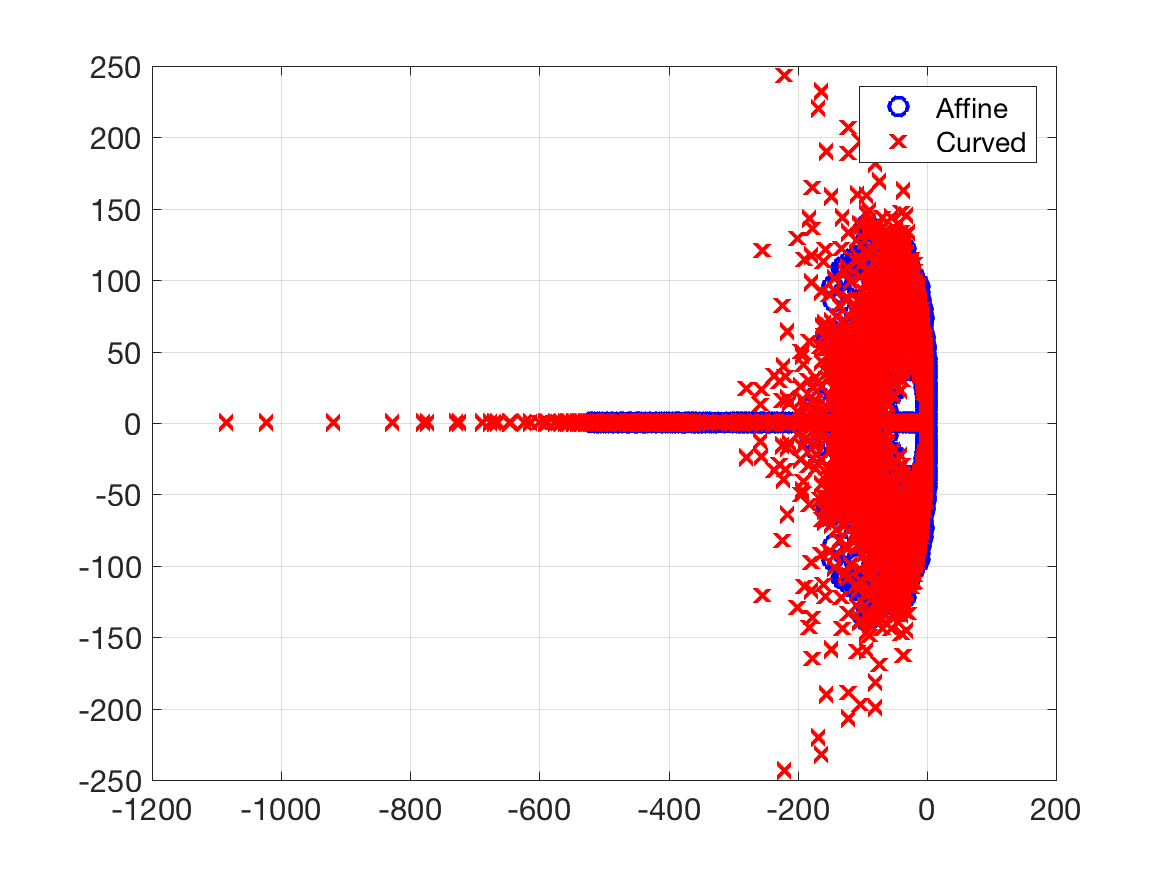
\includegraphics[width=.475\textwidth]{figs/eig_curved_tau1.png}}
\caption*{A skew-symmetric discretization guarantees discrete energy stability.}
\end{figure}

}


\frame{
\frametitle{Elastic wave propagation: 3D isotropic media}
\setcounter{subfigure}{0}
\begin{figure}
\begin{overlayarea}{\textwidth}{.75\textheight}
\only<1>{
\subfloat[Computational mesh]{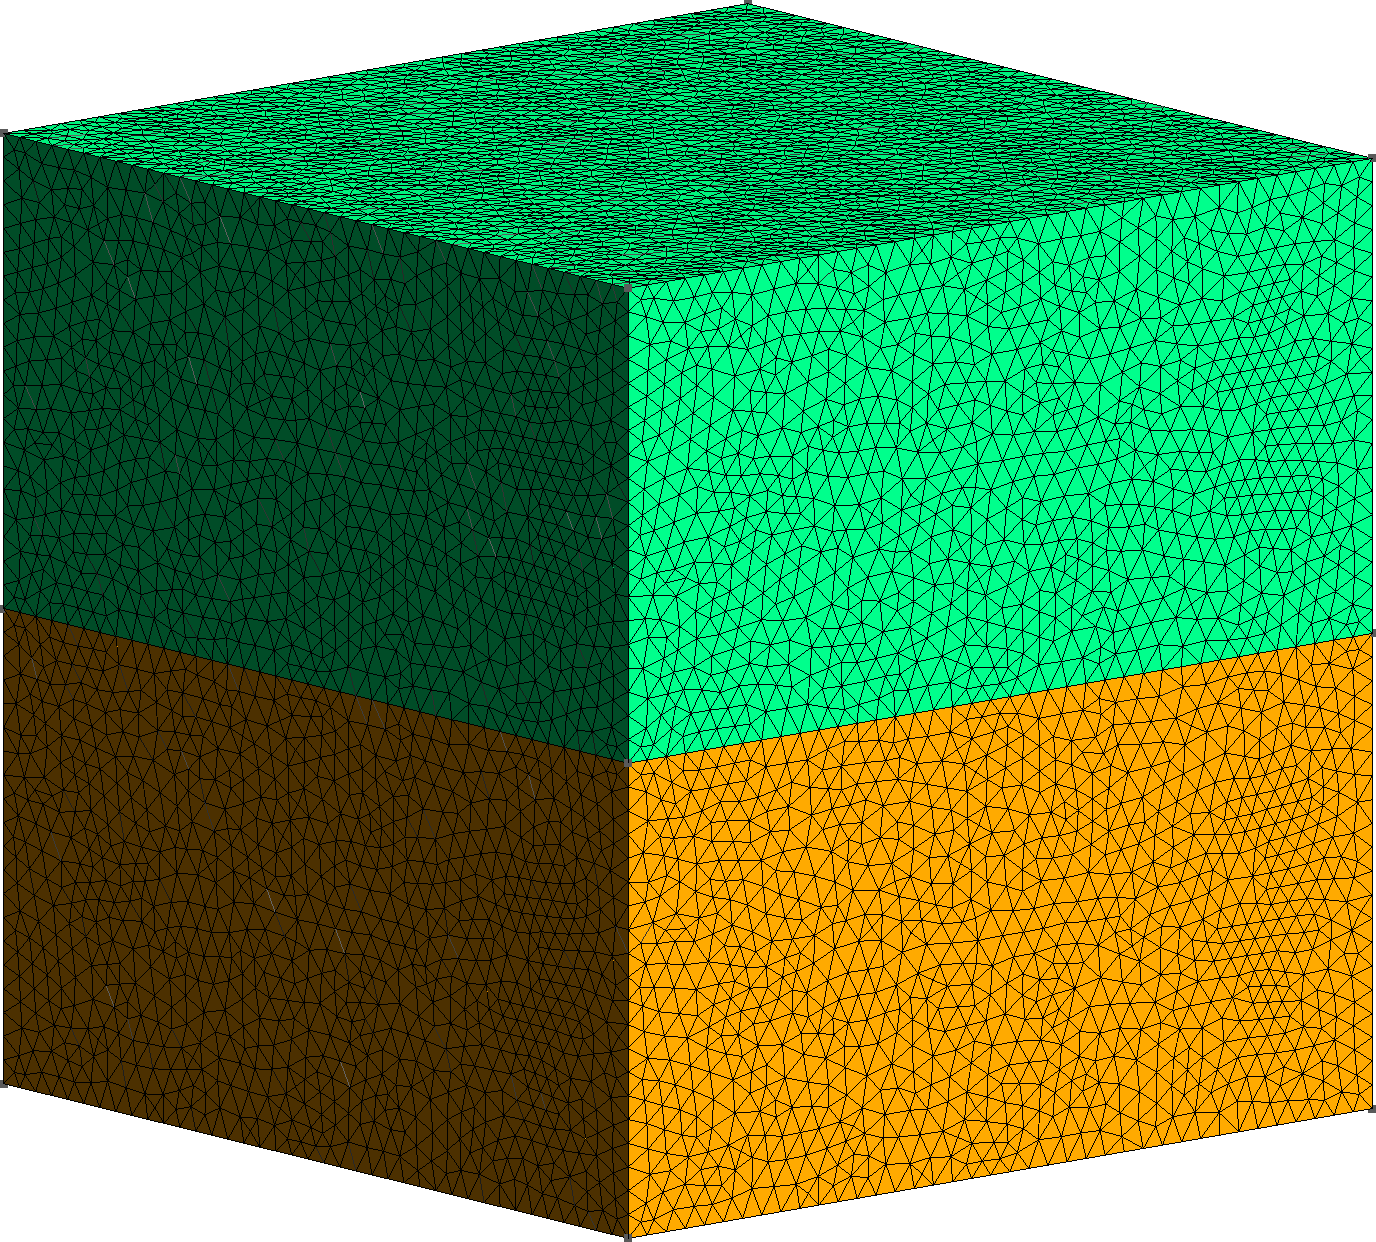
\includegraphics[width=.45\textwidth]{figs/cubeSplitFine.png}}
\hspace{2em}
\subfloat[Homogeneous isotropic media]{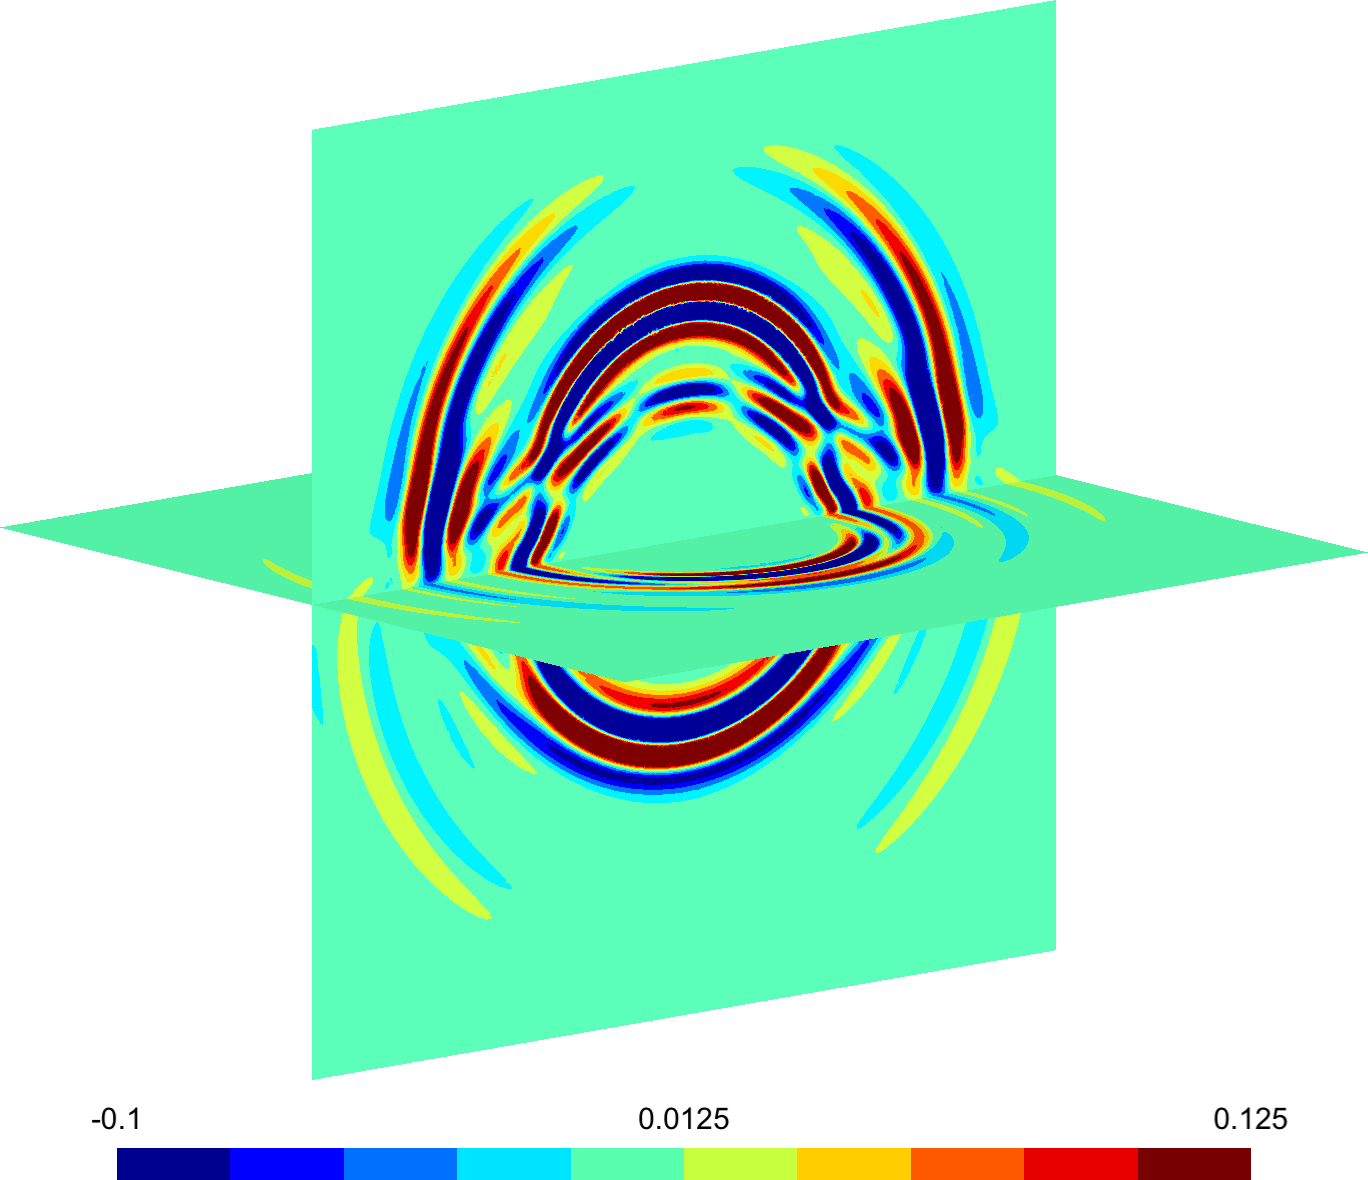
\includegraphics[width=.475\textwidth]{figs/pplane0.png}}
}
\only<2>{
\subfloat[Computational mesh]{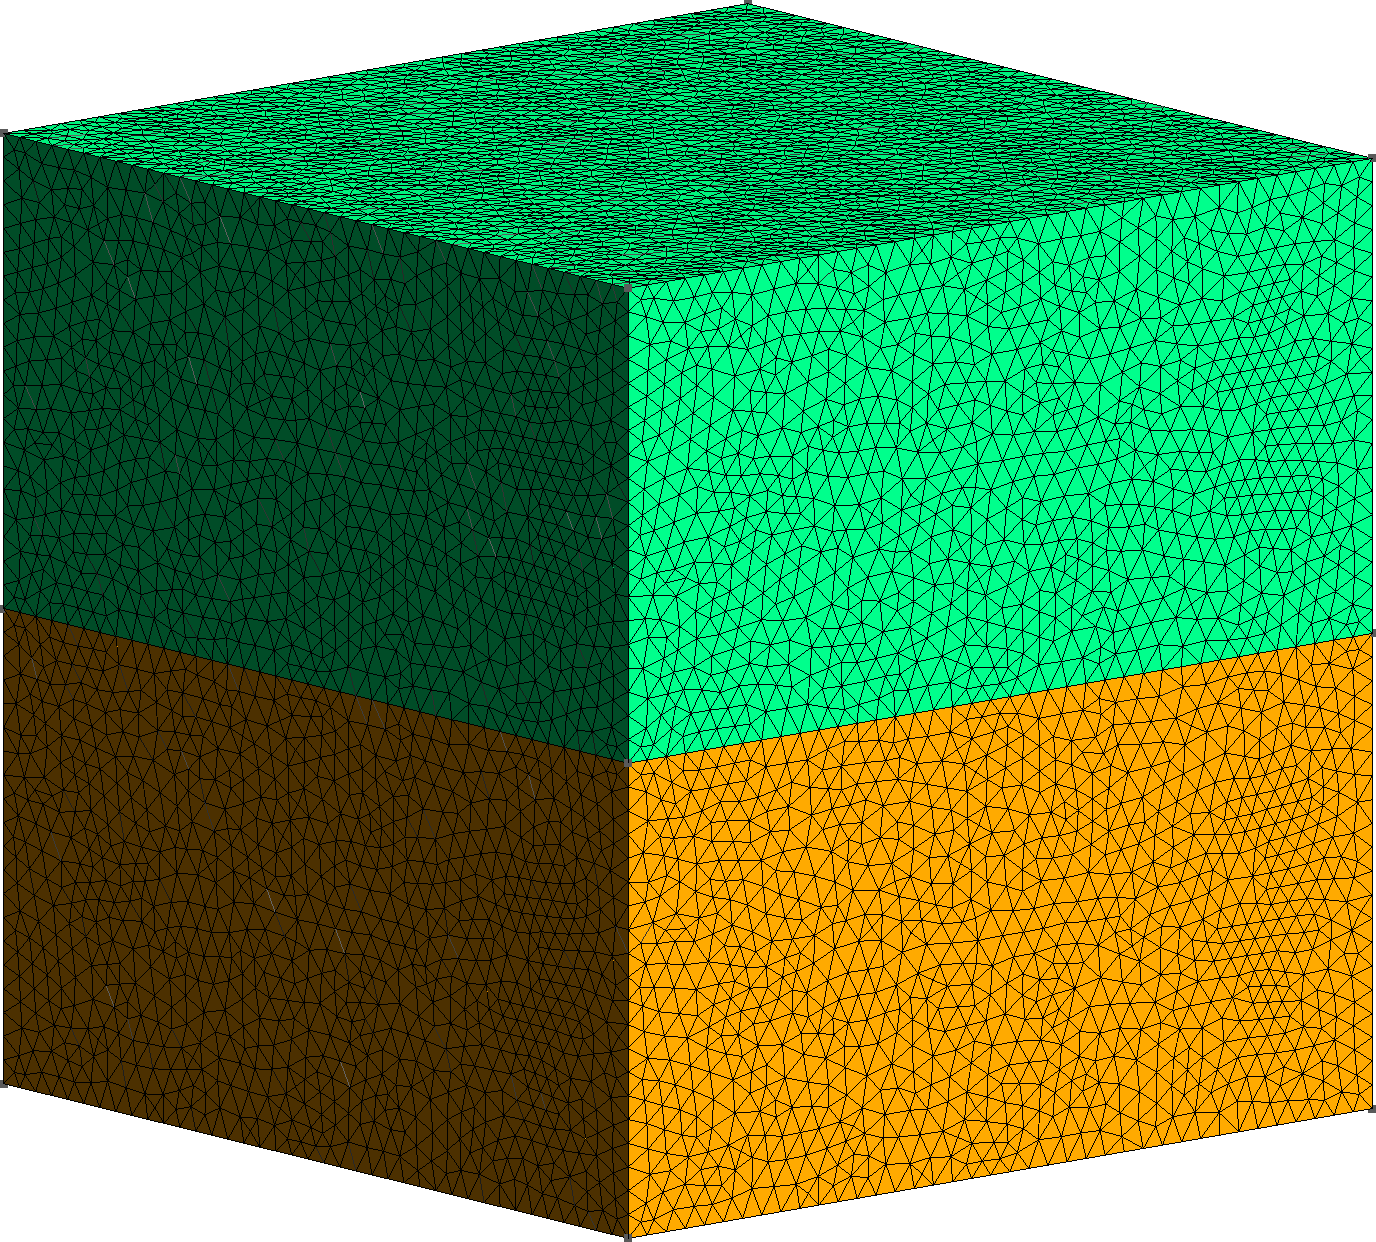
\includegraphics[width=.45\textwidth]{figs/cubeSplitFine.png}}
\hspace{2em}
\subfloat[Piecewise constant $\bm{C}(\bm{x})$]{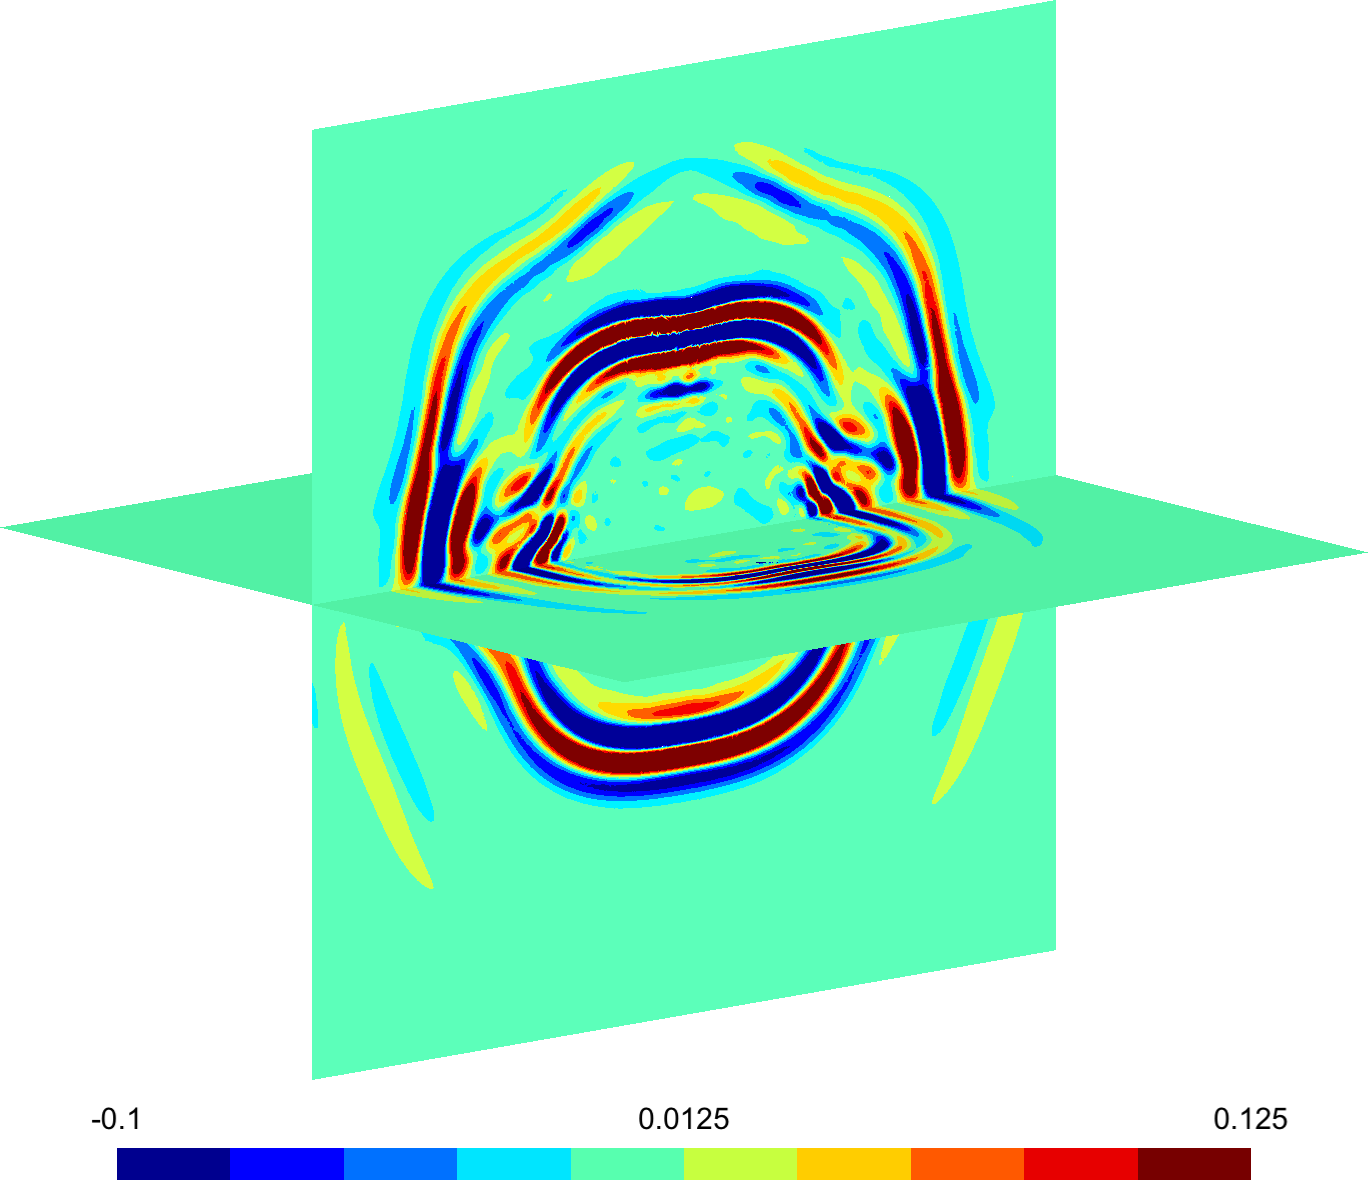
\includegraphics[width=.475\textwidth]{figs/pplanec0.png}}
}
\only<3>{
\subfloat[Computational mesh]{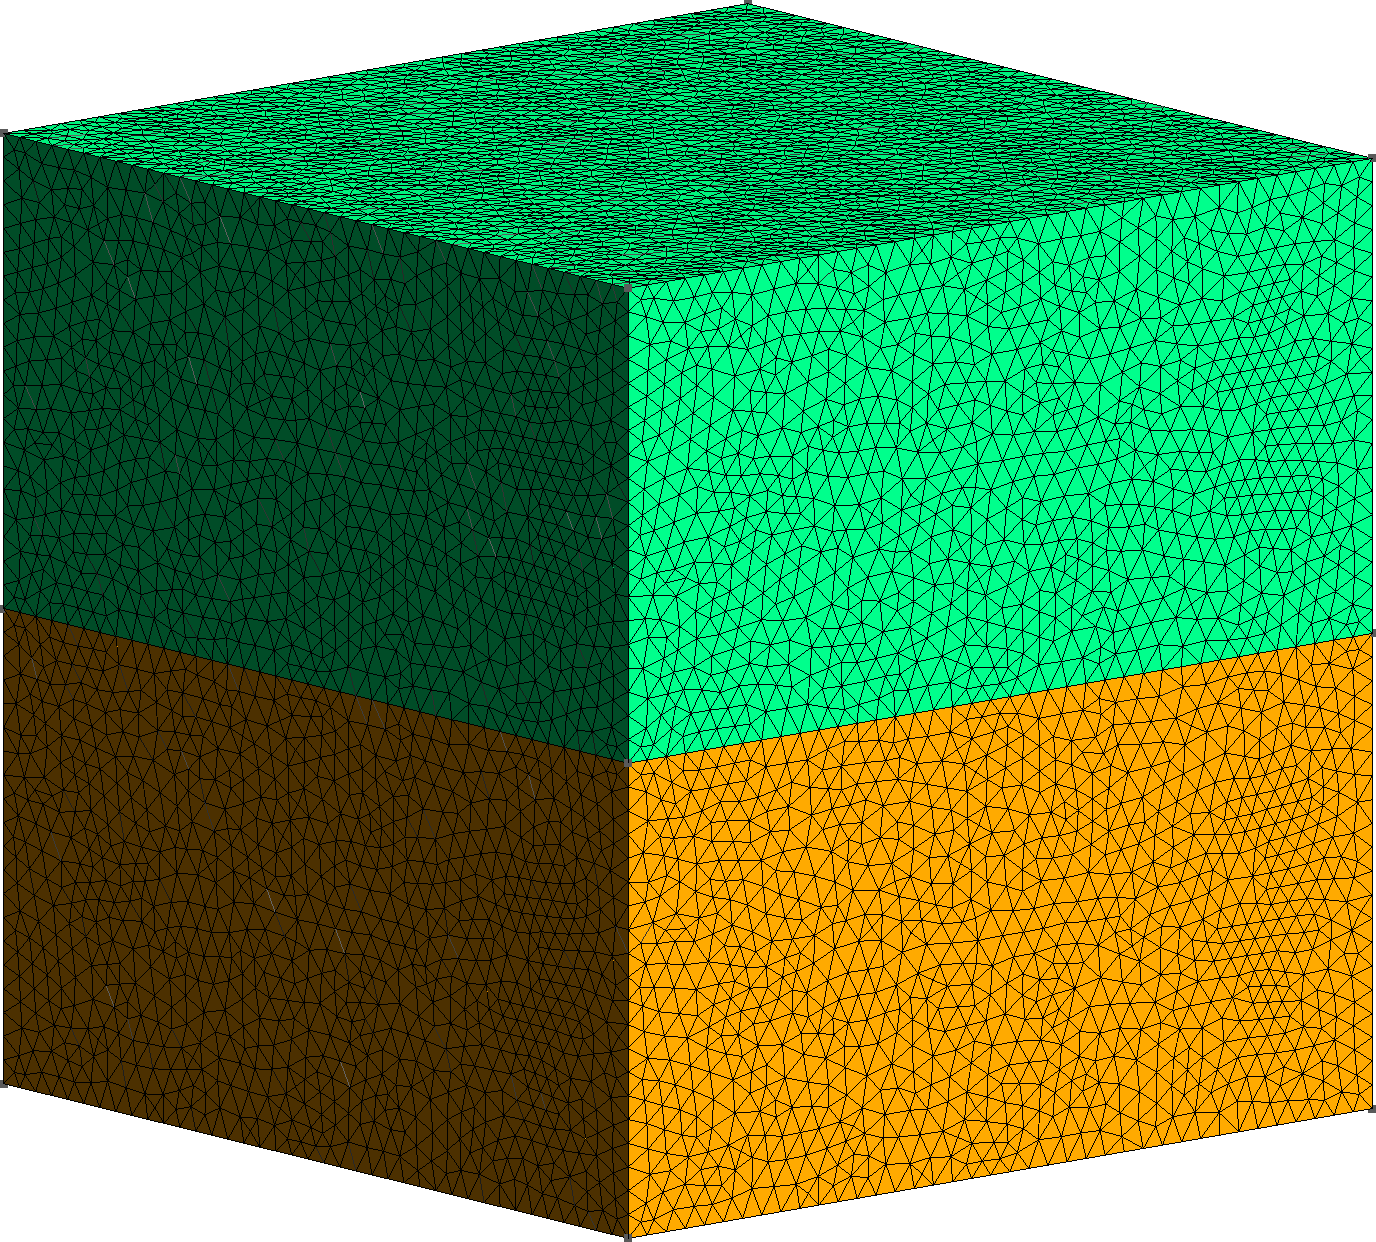
\includegraphics[width=.45\textwidth]{figs/cubeSplitFine.png}}
\hspace{2em}
\subfloat[High order $\bm{C}(\bm{x})$]{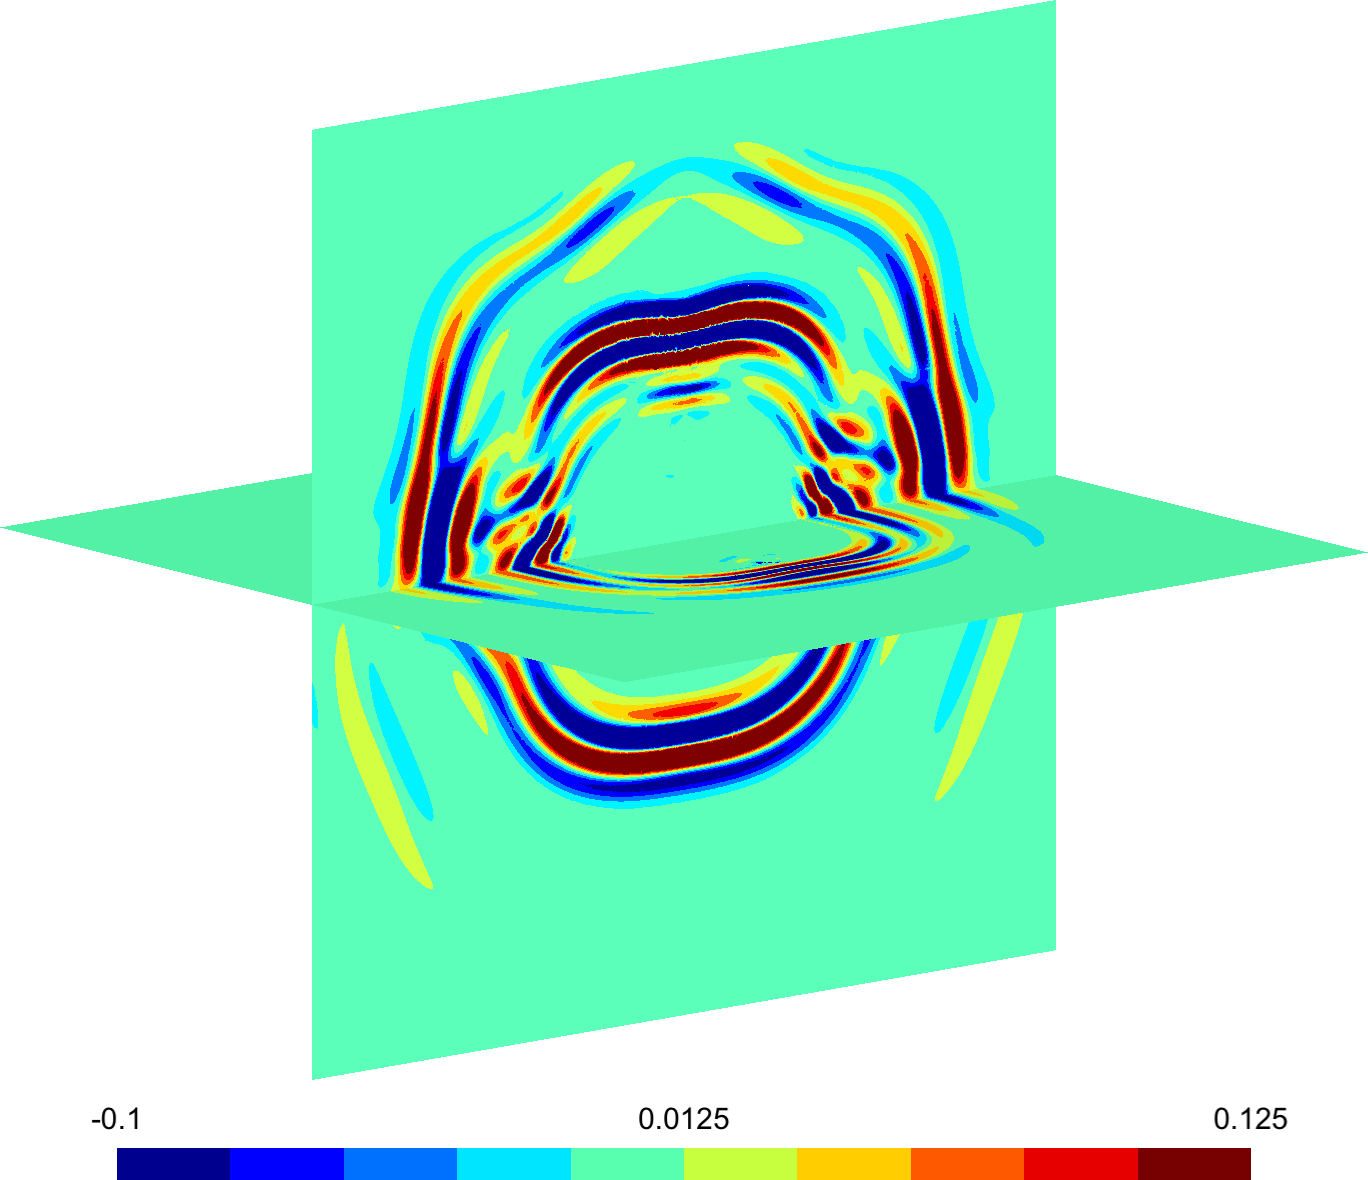
\includegraphics[width=.475\textwidth]{figs/pplanew0.png}}
}
\end{overlayarea}
\caption{${\rm tr}(\bm{\sigma})$ with $\mu(\bm{x}) = 1+ H(y) + \frac{1}{2}\cos(3\pi x)\cos(3\pi y)\cos(3\pi z)$, $N=5$.}
\end{figure}
}

\section{Acoustic-elastic coupling, poroelasticity}

\begin{frame}[noframenumbering]
    \frametitle{Outline}
    \tableofcontents[currentsection]
\end{frame}


\frame{
\frametitle{Acoustic-elastic coupling}
\setcounter{subfigure}{0}

\begin{itemize}
\item Coupling conditions for fluid (acoustic) and solid (elastic) media:
\[
\bm{S} \cdot \bm{n} = p\bm{n}, \qquad \bm{v}\cdot{\bm{n}} = \bm{u}\cdot\bm{n}.
\]
\vspace{.1em}
\item Replace $\jump{p}$ and $\jump{\bm{\sigma}}$ with residuals of coupling conditions
\begin{alignat*}{2}
\jump{p} &= \bm{n}\cdot \LRp{\bm{S}^+\cdot \bm{n}} - p,  \qquad &&\text{(acoustic side)}\\
\bm{A}_n^T\jump{\bm{\sigma}} = \jump{\bm{S}}\cdot\bm{n} &= p^+\bm{n} - \bm{S}\cdot\bm{n}, \qquad &&\text{(elastic side)}.
\end{alignat*}
\vspace{.1em}
\item Energy stable for arbitrary acoustic and elastic media.  
\end{itemize}
%\vspace{-.5em}

%\let\thefootnote\relax\footnotetext{\tiny Ye et al.\ 2016. A DG method with a modified penalty flux for the propagation and scattering of acousto-elastic waves.}
}

\frame{
\frametitle{Acoustic-elastic coupling: arbitrary heterogeneous media}
\begin{overlayarea}{\textwidth}{.65\textheight}
\begin{figure}
\centering
\only<1>{\subfloat[Low order $c^2(\bm{x}), \mu(\bm{x})$]{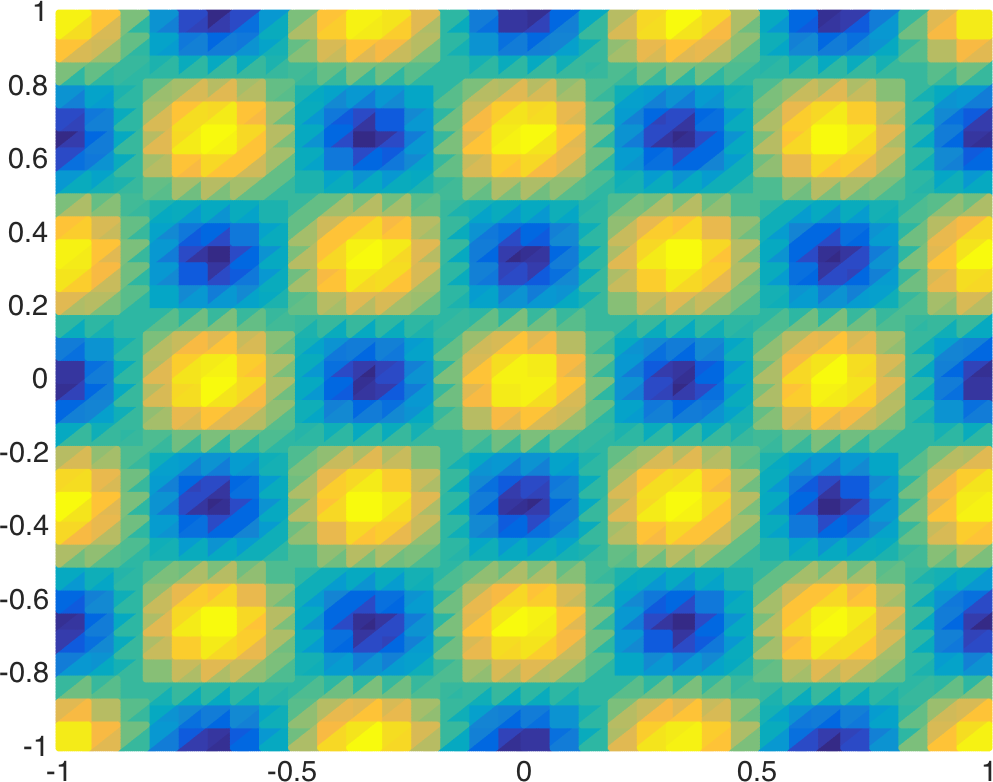
\includegraphics[width=.43\textwidth]{figs/c2muP0.png}}
\hspace{1.5em}
\subfloat[${\rm tr}(\bm{\sigma})$]{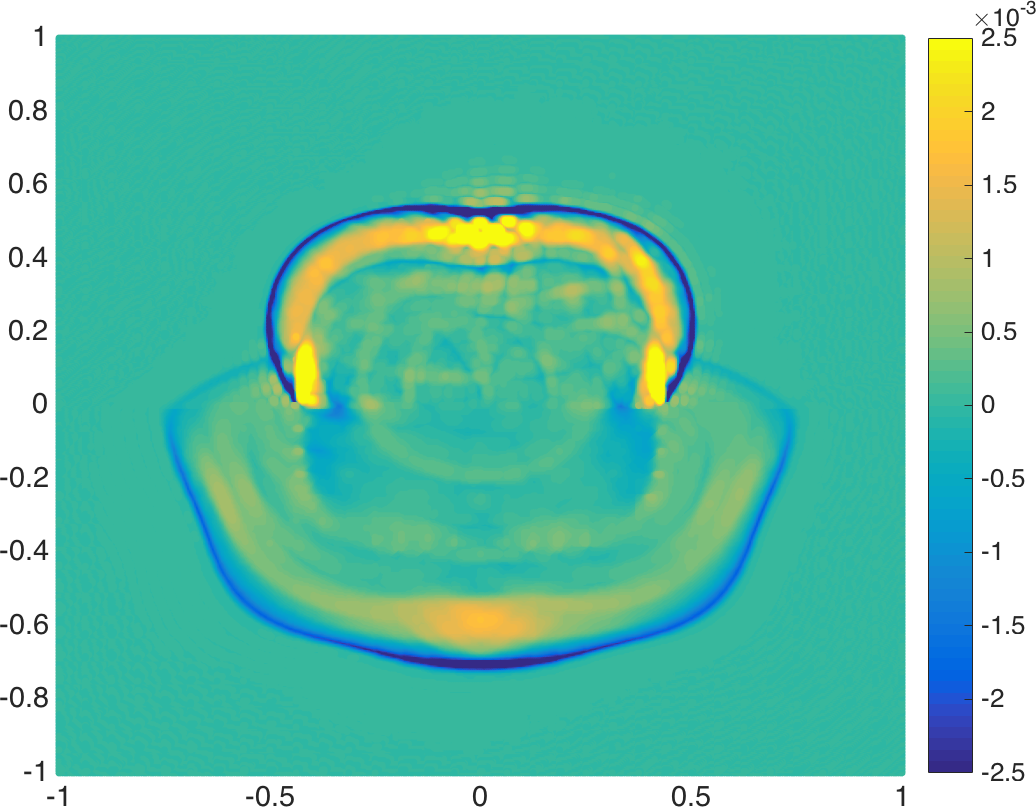
\includegraphics[width=.45\textwidth]{figs/acousticElasticPulseP0.png}}
\caption{Acoustic-elastic waves from a Ricker pulse ($N=10$, $h = 1/16$).}
}
\only<2>{\subfloat[High order $c^2(\bm{x}), \mu(\bm{x})$]{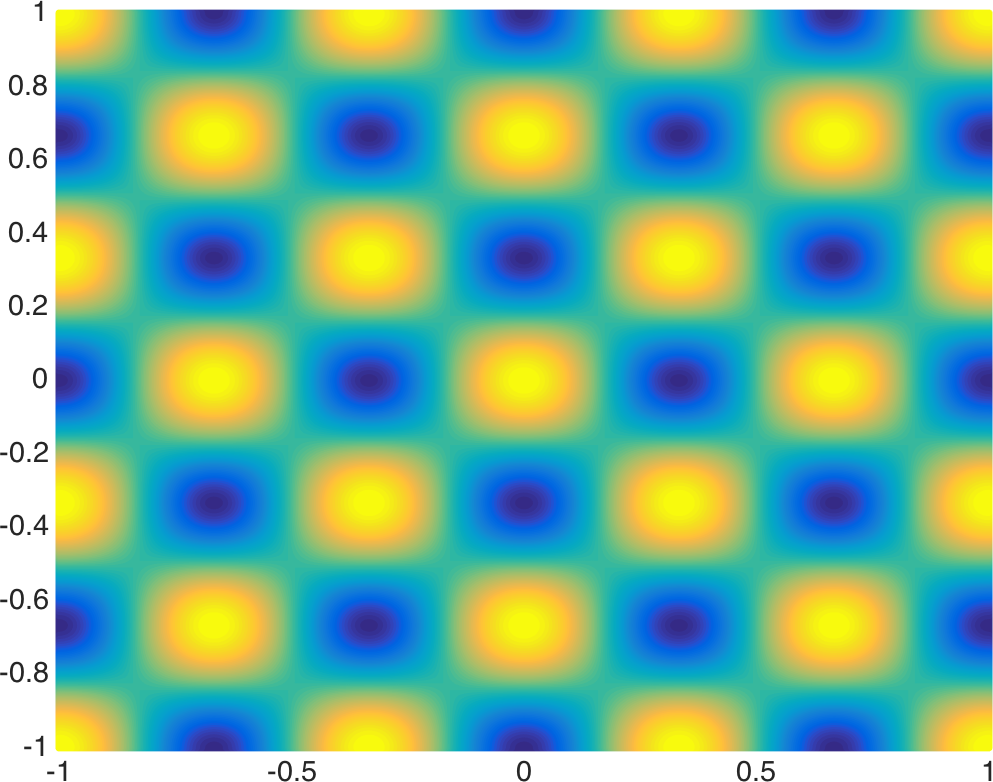
\includegraphics[width=.43\textwidth]{figs/c2mu.png}}
\hspace{1.5em}
\subfloat[${\rm tr}(\bm{\sigma})$]{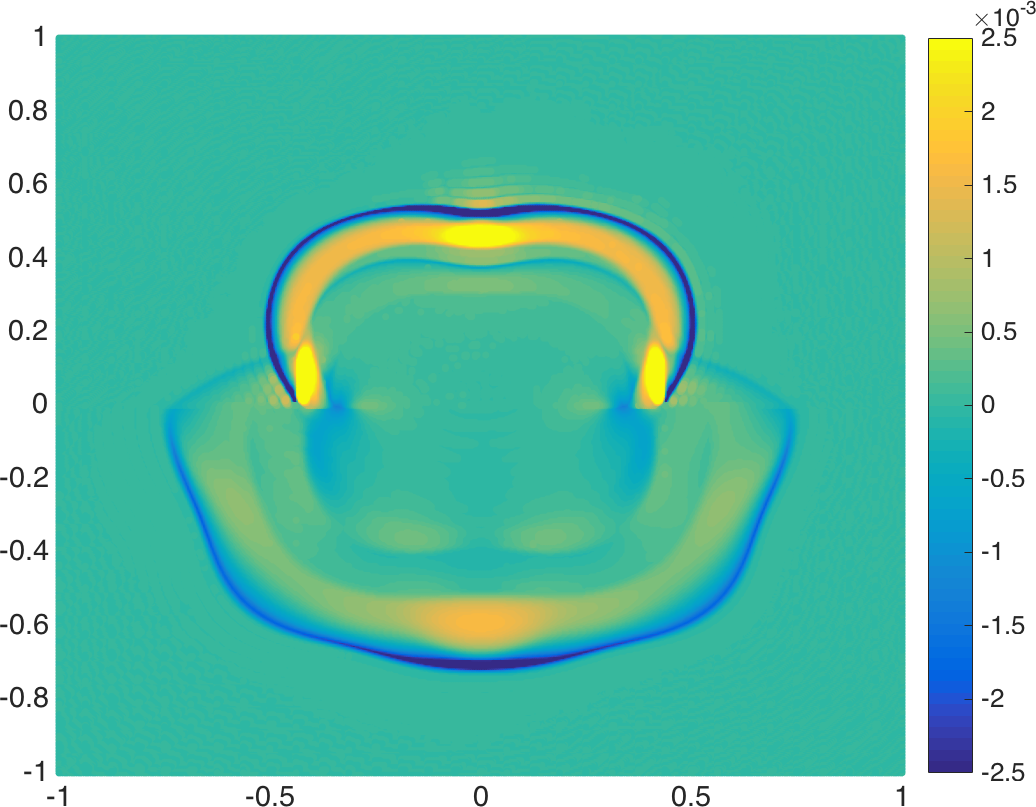
\includegraphics[width=.45\textwidth]{figs/acousticElasticPulseP10.png}}
\caption{Acoustic-elastic waves from a Ricker pulse ($N=10$, $h = 1/16$).}
}
\end{figure}
\end{overlayarea}
}

\frame{
\frametitle{Poroelasticity: low frequency Biot's system}

\begin{itemize}
\item Biot's system adds pore pressure $p$ and relative fluid velocity $\bm{q}$.
\item Symmetric first order system with augmented stress, velocity.
\begin{gather*}
\tilde{\bm{\sigma}} = \LRp{\sigma_{xx},\sigma_{yy},\sigma_{zz},\sigma_{yz},\sigma_{xz},\sigma_{xy}, p}^T, \quad \tilde{\bm{v}} = \LRp{v_x, v_y, v_z, q_x, q_y, q_z}^T\\
\bm{E}_v\pd{\tilde{\bm{v}}}{t}{} = \sum_{i=1}^d \bm{A}_i^T \pd{\tilde{\bm{\sigma}}}{\bm{x}_i}{} - \bm{D}\tilde{\bm{v}}, \qquad \bm{E}_{\sigma}\pd{\tilde{\bm{\sigma}}}{t}{} = \sum_{i=1}^d \bm{A}_i \pd{\tilde{\bm{v}}}{\bm{x}_i}{}.
\end{gather*}
\item $\bm{E}_s, \bm{E}_v$ SPD, $\bm{A}_i$ spatially const.\ + sparse (a single $\pm 1$ per row).
\[
\bm{E}_v = \begin{pmatrix}
\rho & & \rho_f &\\
 & \ddots & & \ddots  \\
\rho_f  & & m_1   & \\
  & \ddots &  & \ddots   \\
\end{pmatrix}, \quad \bm{E}_s = \begin{pmatrix}
\bm{C}^{-1} & \bm{C}^{-1}\bm{\alpha}\\
\bm{\alpha}^T\bm{C}^{-1} & \frac{1}{M} + \bm{\alpha}^T\bm{C}^{-1}\bm{\alpha}
\end{pmatrix}, \qquad 
\]
\end{itemize}

\let\thefootnote\relax\footnotetext{\tiny Lemoine, Ou, LeVeque 2013. High-resolution finite volume modeling of wave propagation in orthotropic poroelastic media.}
}



\frame{
\frametitle{Numerical results for Biot (with de Hoop, Shukla)}

\vspace{-2em}
\begin{figure}
\centering
%\begingroup
%\captionsetup[subfloat]{width=.34\columnwidth}
\subfloat[\scriptsize Orthotropic media, 1.56 ms]{
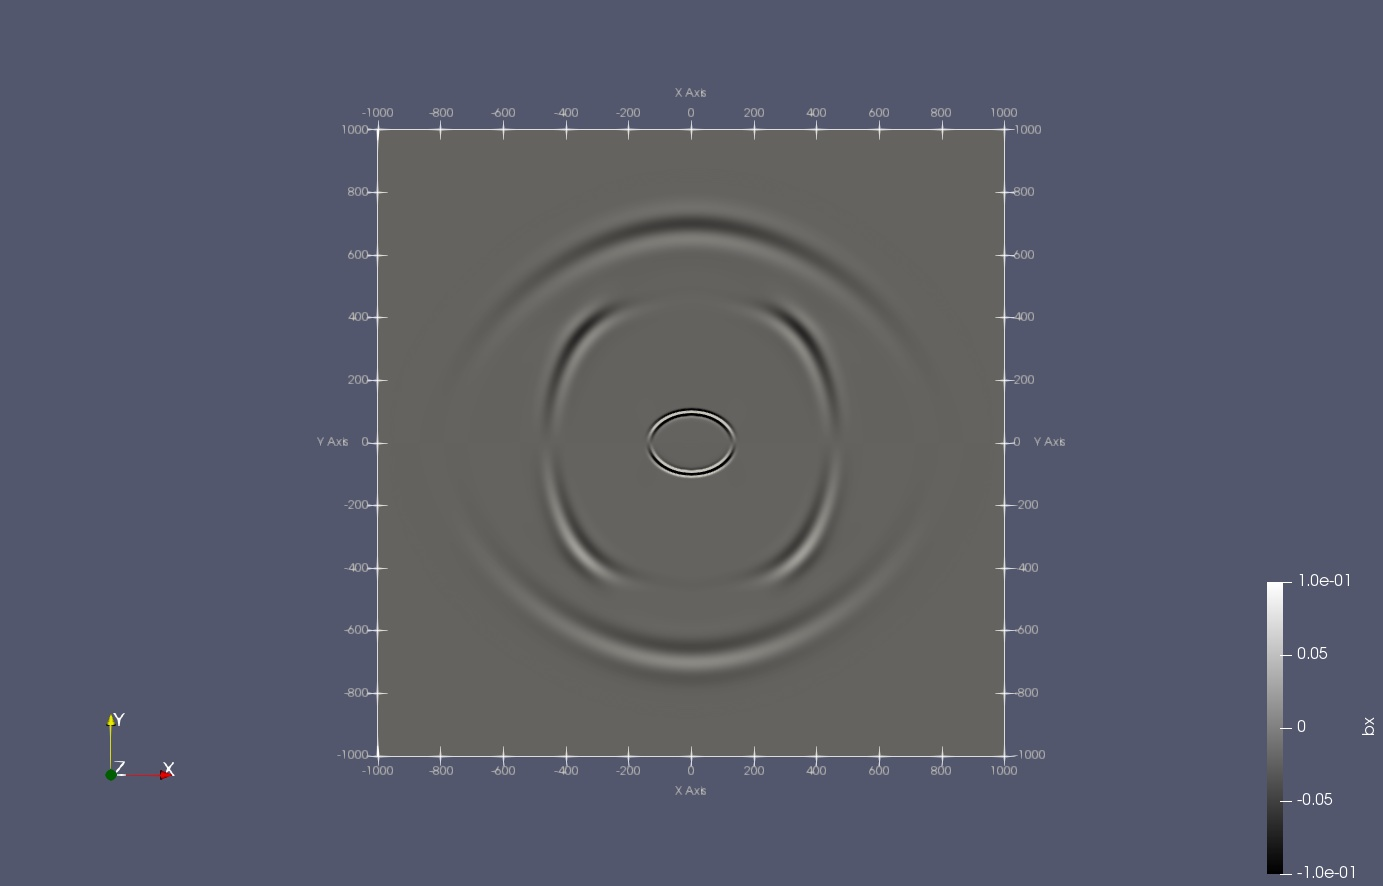
\includegraphics[trim={11cm, 3cm, 11cm, 3cm}, clip, width=0.33\columnwidth]{figs/HF_inviscid_ortho_bz_3730HZ.jpg}
}
\subfloat[\scriptsize Epoxy-glass, 1.8 ms]{
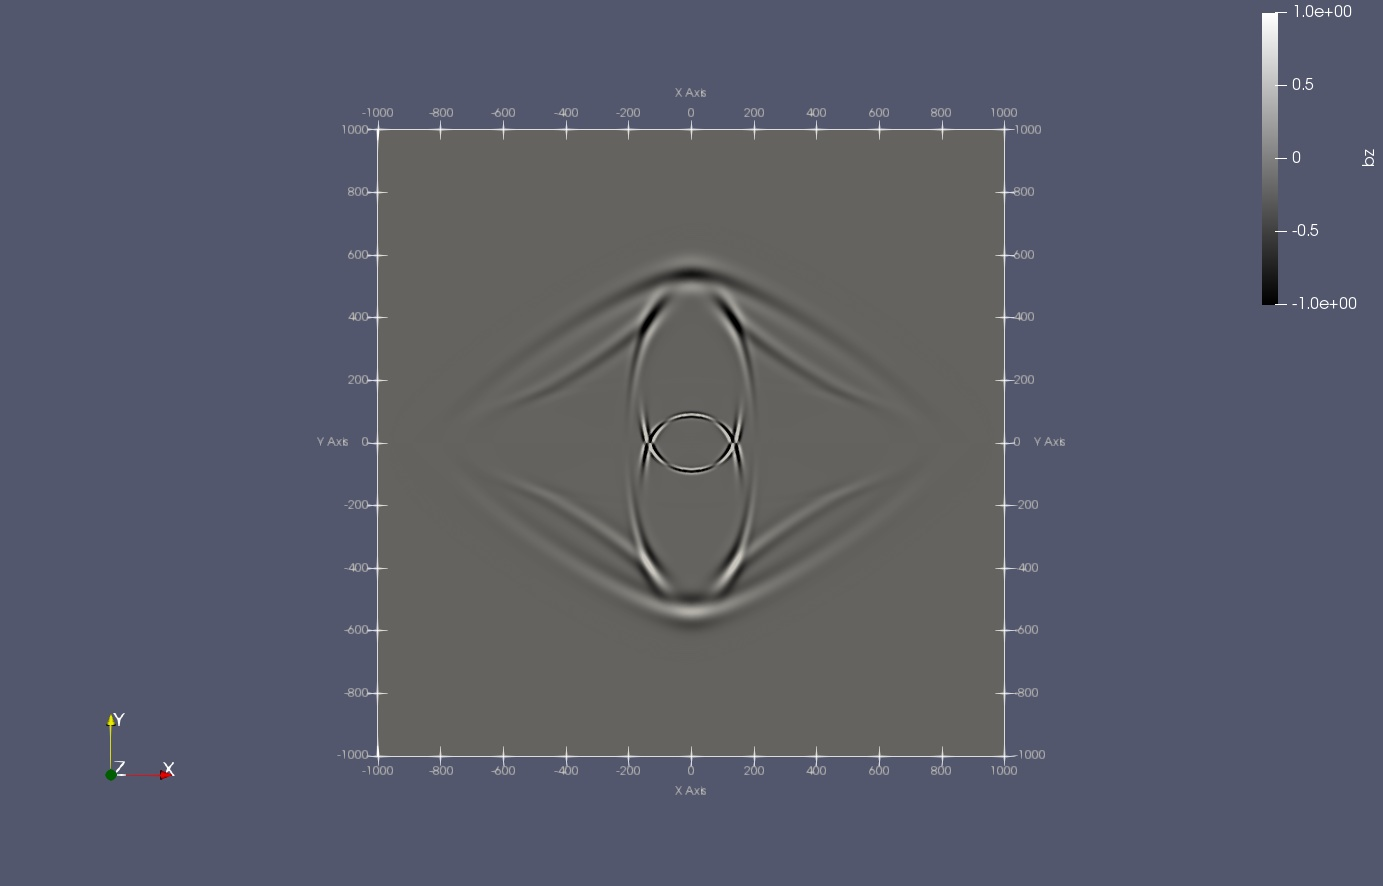
\includegraphics[trim={11cm, 3cm, 11cm, 3cm}, clip, width=0.33\columnwidth]{figs/HF_viscid_epoxy_bz_3730HZ.jpg}
}
\subfloat[\scriptsize Isotropic interface, 230 ms]{
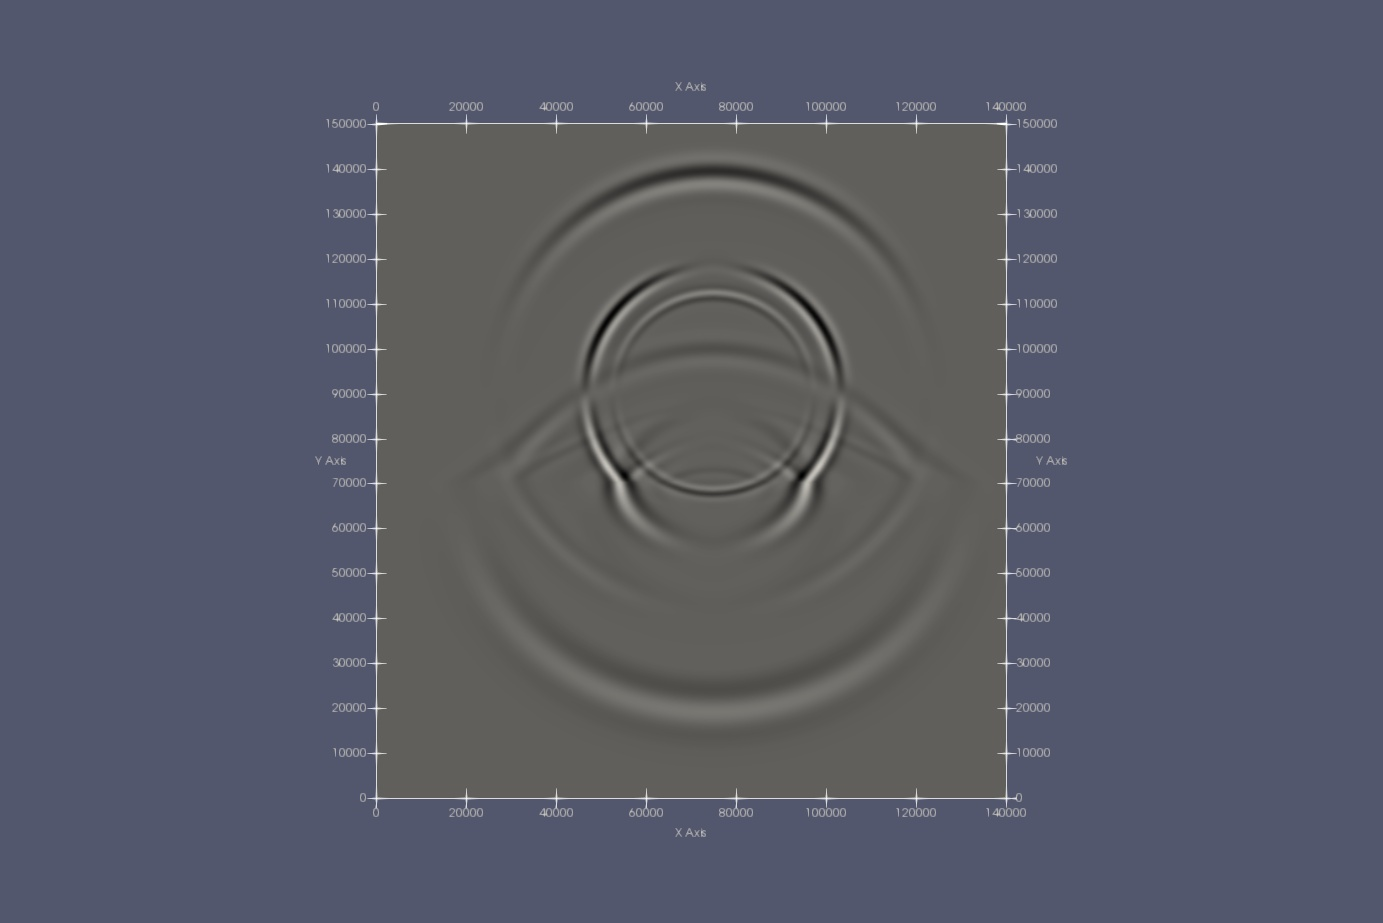
\includegraphics[trim={11cm, 3cm, 11cm, 3cm}, clip, width=0.314\columnwidth]{figs/interface_model.jpg}
}
%\endgroup
\caption*{Inviscid Biot solution (mass particle velocity) showing fast P, slow S, and slow P waves.  Simulation utilizes $N = 3$ and a uniform mesh of $128$ elements per side.}
\end{figure}

\begin{center}
Systematic derivation of WADG formulations: can symmetrize a system by defining an appropriate convex entropy (energy function).
\end{center}

\let\thefootnote\relax\footnotetext{\tiny Carcione 1996. Wave propagation in anisotropic, saturated porous media: plane wave theory and numerical simulation.}
\let\thefootnote\relax\footnotetext{\tiny Lemoine, Ou, LeVeque 2013. High-resolution finite volume modeling of wave propagation in orthotropic poroelastic media.}
}


\frame{
\frametitle{Summary and acknowledgements}

\begin{itemize}
\item Weight-adjusted DG (WADG) for acoustic and elastic wave propagation in heterogeneous media and on curved meshes.
\vspace{.25em}
\item Generalized mass lumping: energy stability and high order accuracy.
\vspace{.25em}
\item Significantly simpler formulations using symmetric forms of PDEs.
\vspace{.25em}
\item This work is supported by DMS-1719818 and DMS-1712639. 
\end{itemize}
\vspace{.25em}
\begin{center}
Thank you!  Questions?
\vspace{.25em}

{
\includegraphics[width=.15\textwidth]{figs/nsf.jpg}}
\end{center}

\let\thefootnote\relax\footnotetext{\tiny Chan, Hewett, Warburton.\ 2017.  {Weight-adjusted DG methods: wave propagation in heterogeneous media} (SISC).}
\let\thefootnote\relax\footnotetext{\tiny Chan 2018.  Weight-adjusted DG methods: matrix-valued weights and elastic wave prop.\ in heterogeneous media (IJNME).}
}


\begin{frame}[noframenumbering]
\frametitle{Additional slides }
\end{frame}

\frame[noframenumbering]{
%\frametitle{Nodal tetrahedra at high order}
\frametitle{Computational costs at high orders of approximation}

%\begin{itemize}
%%\item Hexahedra: tensor product structure $\rightarrow$ $O(N^4)$ vs $O(N^6)$ local cost.
%%\item How do (naively implemented) nodal tetrahedra behave at high order?
%\item 
%\end{itemize}
%\vspace{-.25em}
\begin{center}
Note: WADG at high orders becomes \textbf{expensive}!
\end{center}
\vspace{-.5em}
\begin{columns}
\begin{column}{.55\textwidth}
\begin{figure}
\centering
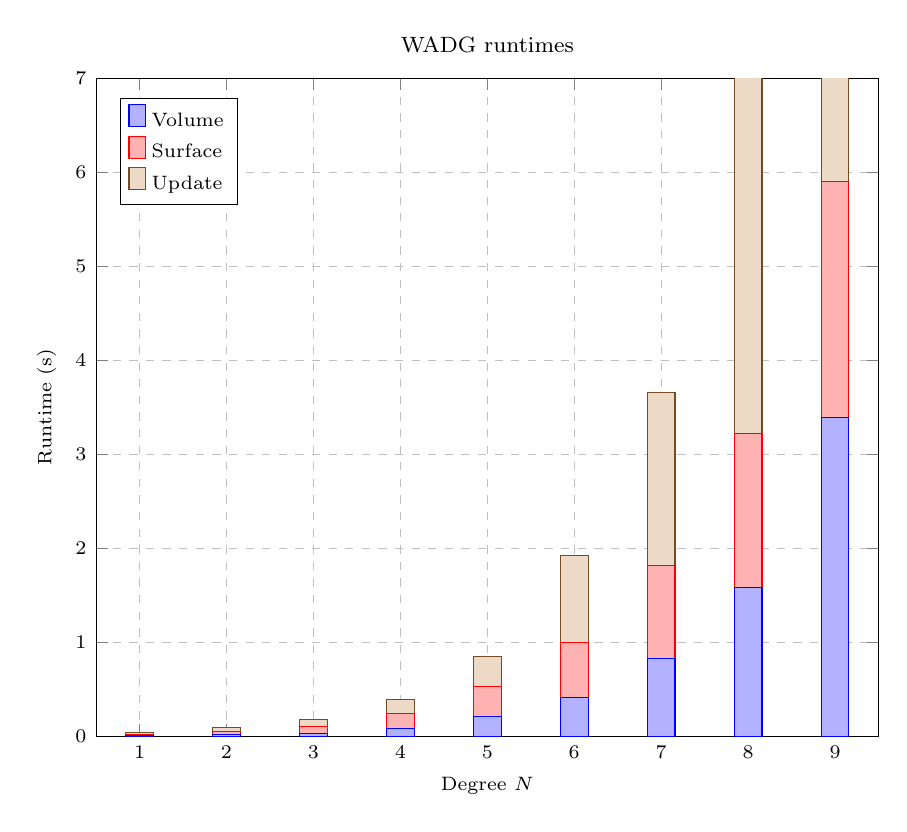
\begin{tikzpicture}
\begin{axis}[
	width=.95\textwidth,
	legend cell align=left,
	%title={Runtime (NPT nodal)},
	title={WADG runtimes},
	xlabel={Degree $N$},
	ylabel={Runtime (s)},
	xmin=.5, xmax=9.5,
	ymin=0,ymax=7,
	ybar stacked,
%	nodes near coords,
	%xmin=.5, xmax=9.5,
	xtick={1,2,3,4,5,6,7,8,9},
	legend pos=north west,
	xmajorgrids=true,
	ymajorgrids=true,
	grid style=dashed,
] 
%nodal runtimes
\addplot coordinates{(1,0.00529)(2,0.0135)(3,0.0302)(4,0.0854)(5,0.206)(6,0.41)(7,0.829)(8,1.58)(9,3.39)};
\addplot coordinates{(1,0.0121)(2,0.0403)(3,0.0722)(4,0.158)(5,0.322)(6,0.587)(7,0.987)(8,1.64)(9,2.51)};
%\addplot coordinates{(1,0.00289997)(2,0.00707789)(3,0.0211354)(4,0.0683213)(5,0.211452)(6,0.530006)(7,1.11929)};
%\addplot coordinates{(1,0.0242951)(2,0.0510198)(3,0.0916193)(4,0.183583)(5,0.397246)(6,1.15212)(7,2.30179)(8,14.2639)};
\addplot coordinates{(1,0.0194361)(2,0.0408158)(3,0.0732955)(4,0.146866)(5,0.317797)(6,0.921698)(7,1.84143)(8,11.4111)(9,21)};


%\addplot coordinates{(1,0.009394)(2,0.025607)(3,0.046205)(4,0.080841)(5,0.142045)(6,0.19389)(7,0.27628)(8,0.381)(9,0.5088)};
%\addplot coordinates{(1,0.026784)(2,0.079407)(3,0.148605)(4,0.324241)(5,0.670045)(6,1.19089)(7,2.09228)(8,3.601)(9,6.4088)};

\legend{Volume, Surface, Update}
%\legend{Volume, Surface}
\end{axis}
\end{tikzpicture}
%\caption*{Per-kernel runtimes for tetrahedra with nodal basis.  Runtimes are recorded for ten RK4 timesteps on a mesh of 98304 elements.}
%\caption*{DG runtimes for 50 timesteps and 98304 elements.}
\caption*{\scriptsize WADG runtimes for 50 timesteps, 98304 elements.}
\end{figure}
\end{column}
\begin{column}{.45\textwidth}
\vspace{-2em}
\begin{itemize}
\item Large \textbf{dense} matrices: $O(N^6)$ work per tet.
\vspace{1em}
\item High orders usually use tensor-product elements: $O(N^{4})$ vs $O(N^{6})$ cost, but less geometric flexibility.
\vspace{1em}
\item Idea: choose basis such that matrices are \textbf{sparse}.
%\item $O(N^{4})$ vs $O(N^6)$ cost, but less geometric flexibility.
\end{itemize}
\end{column}
\end{columns}
}

\frame[noframenumbering]{
\frametitle{BBDG: efficient volume, surface kernels}

\vspace{-.5em}
%\begin{center}
%Bernstein-Bezier DG achieves $\approx 2\times$ speedup at moderate orders,\\ and up to $\approx 6\times$ speedup at high orders.
%\end{center}
%\begin{center}
%Bernstein-Bezier DG achieves $\approx 2\times$ speedup at moderate orders,\\ and up to $4\times$ speedup at high orders.
%\end{center}
\vspace{-1em}
\begin{figure}
\centering
\only<1>{
\hspace{-1em}
\subfloat{
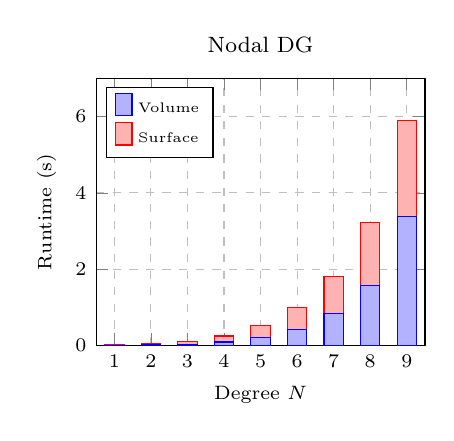
\begin{tikzpicture}
\begin{axis}[
	width=.475\textwidth,
	legend cell align=left,
	title={Nodal DG},
	xlabel={Degree $N$},
	ylabel={Runtime (s)},
	xmin=.5, xmax=9.5,
	ymin=0,ymax=7,
	ybar stacked,
	    bar width=7pt,
	legend style={font=\tiny},	
	xtick={1,2,3,4,5,6,7,8,9},
	legend pos=north west,
	xmajorgrids=true,
	ymajorgrids=true,
	grid style=dashed,
] 
%nodal runtimes
\addplot coordinates{(1,0.00529)(2,0.0135)(3,0.0302)(4,0.0854)(5,0.206)(6,0.41)(7,0.829)(8,1.58)(9,3.39)};
\addplot coordinates{(1,0.0121)(2,0.0403)(3,0.0722)(4,0.158)(5,0.322)(6,0.587)(7,0.987)(8,1.64)(9,2.51)};
%\addplot coordinates{(1,0.009394)(2,0.025607)(3,0.046205)(4,0.080841)(5,0.142045)(6,0.19389)(7,0.27628)(8,0.381)(9,0.5088)};

\legend{Volume, Surface}%, Update}

\end{axis}
\end{tikzpicture}
}
\hspace{1em}
\subfloat{
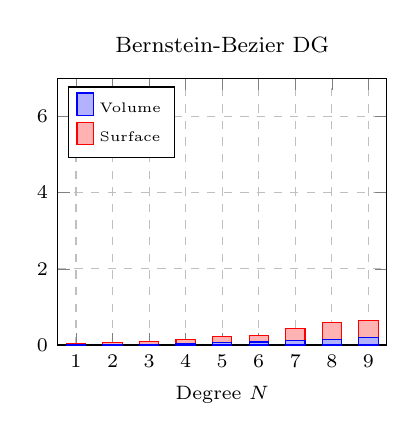
\begin{tikzpicture}
\begin{axis}[
	width=.475\textwidth,
	legend cell align=left,
	title={Bernstein-Bezier DG },
	xlabel={Degree $N$},
	legend style={font=\tiny},	
%	ylabel={Runtime (s)},
	xmin=.5, xmax=9.5,
	ymin=0,ymax=7,
	ybar stacked,
	    bar width=7pt,
	xtick={1,2,3,4,5,6,7,8,9},
	legend pos=north west,
	xmajorgrids=true,
	ymajorgrids=true,
	grid style=dashed,
] 
%bern runtimes
\addplot 
coordinates{(1,0.00564)(2,0.0119)(3,0.0203)(4,0.034)(5,0.0593)(6,0.0791)(7,0.112)(8,0.155)(9,0.204)};
\addplot 
coordinates{(1,3.45E-02)(2,5.15E-02)(3,6.61E-02)(4,1.03E-01)(5,1.76E-01)(6,1.73E-01)(7,3.32E-01)(8,4.48E-01)(9,4.31E-01)};
%\addplot 
%coordinates{(1,0.0093767)(2,0.0255921)(3,0.04623)(4,0.081)(5,0.14229)(6,0.194133)(7,0.277041)(8,0.38163)(9,0.50694)};

\legend{Volume, Surface}%, Update}

\end{axis}
\end{tikzpicture}
}
%\caption*{Per-kernel runtimes for nodal and Bernstein-Bezier bases.  Runtimes are recorded for ten RK4 timesteps on a mesh of 98304 elements.}
%\caption*{Kernel runtimes for Naive nodal, Blocked nodal, and Bernstein-Bezier DG implementations (50 RHS evaluations, 98304 elements).}
%\caption*{Kernel runtimes for Standard nodal, Blocked nodal, and Bernstein-Bezier DG implementations (50 RHS evaluations, 98304 elements).}
%\caption*{DG runtimes for 50 timesteps, 98304 elements.}
}

% maybe comment out? speedup
\only<2>{
\subfloat{
\begin{tikzpicture}
\begin{axis}[
	width=.5\textwidth,
	legend cell align=left,
	title={BBDG speedup over nodal DG},
	xlabel={Degree $N$},
	ylabel={Speedup},
	xmin=.5, xmax=9.5,
	ymin=0,ymax=8,%17.5,	
        ybar=2*\pgflinewidth,
    bar width=3pt,
	xtick={1,2,3,4,5,6,7,8,9},
	ymin=0,
	legend pos=north west,
	legend style={font=\tiny},
	ymajorgrids=true,
	grid style=dashed,
] 
%speedup V/S
%\addplot table[x=N, y=V] from \runtimeOptNaive;
%\addplot table[x=N, y=S] from \runtimeOptNaive;
\addplot table[x=N, y=V] from \runtimeSpeedupBest;
\addplot table[x=N, y=S] from \runtimeSpeedupBest;
%\addplot table[x=N, y=T] from \runtimeOptNaive;
%\addplot table[x=N, y=Vopt] from \datatable;
\addplot+[draw=black,line legend, very thick,smooth,dashed] coordinates{(0,1)(10,1)};

%\legend{Volume, Surface, Total, Reference (no speedup)}
\legend{Volume, Surface}%, Total}%, No speedup}
\end{axis}
\end{tikzpicture}

}

%\caption*{Ratio of runtimes of volume/surface kernels and total RHS evaluation using a Bernstein-Bezier basis instead of nodal polynomials.}
%\caption*{Speedups achieved over nodal DG by using a Bernstein-Bezier basis.}
}
%\caption*{Bernstein-Bezier DG achieves $\approx 2\times$ speedup at moderate orders,\\ and up to $4\times$ speedup at high orders.}
\end{figure}
%\only<1>{\vspace{-.25em}}
%\only<2>{\vspace{-.5em}}
%\vspace{-.75em}
%\[
%\underbrace{\td{\mathbf{u}}{t}}_{\text{Update kernel}} = \underbrace{\mathbf{D}_x \mathbf{u}}_{\text{Volume kernel}} + \underbrace{\sum_{\text{ faces}}\mathbf{L}_f \LRp{\rm flux}}_{\text{Surface kernel}}, \quad \mathbf{L}_f = \mathbf{{M}}^{-1}\mathbf{{M}}_f.
%\]
\begin{center}
Bernstein-Bezier speedup requires constant coefficient RHS evaluation!
\end{center}
}

\frame[noframenumbering]{
\frametitle{BBWADG: polynomial multiplication and projection}
\setcounter{subfigure}{0}
\vspace{-1em}
\begin{figure}
\centering
\hspace{-1em}
\subfloat[Exact $c^2$]{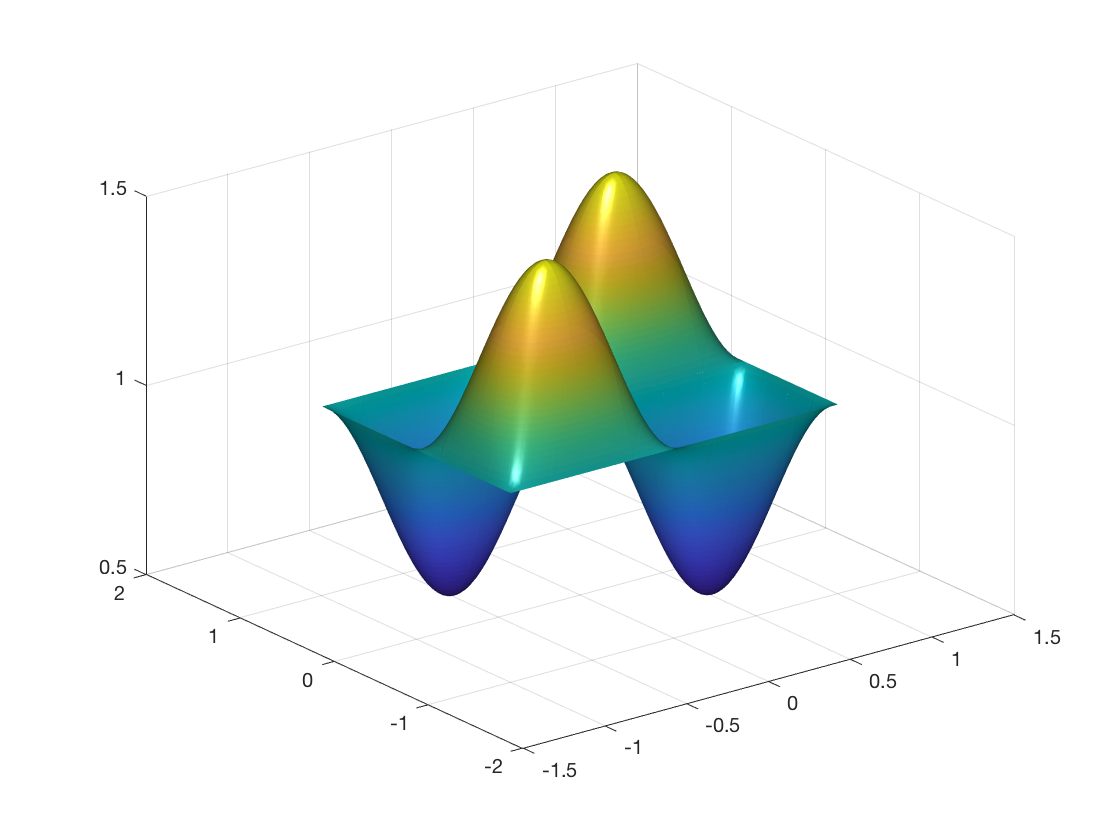
\includegraphics[width=.35\textwidth]{figs/cfunEx.png}}
\hspace{-1em}
\subfloat[$M=0$ approximation]{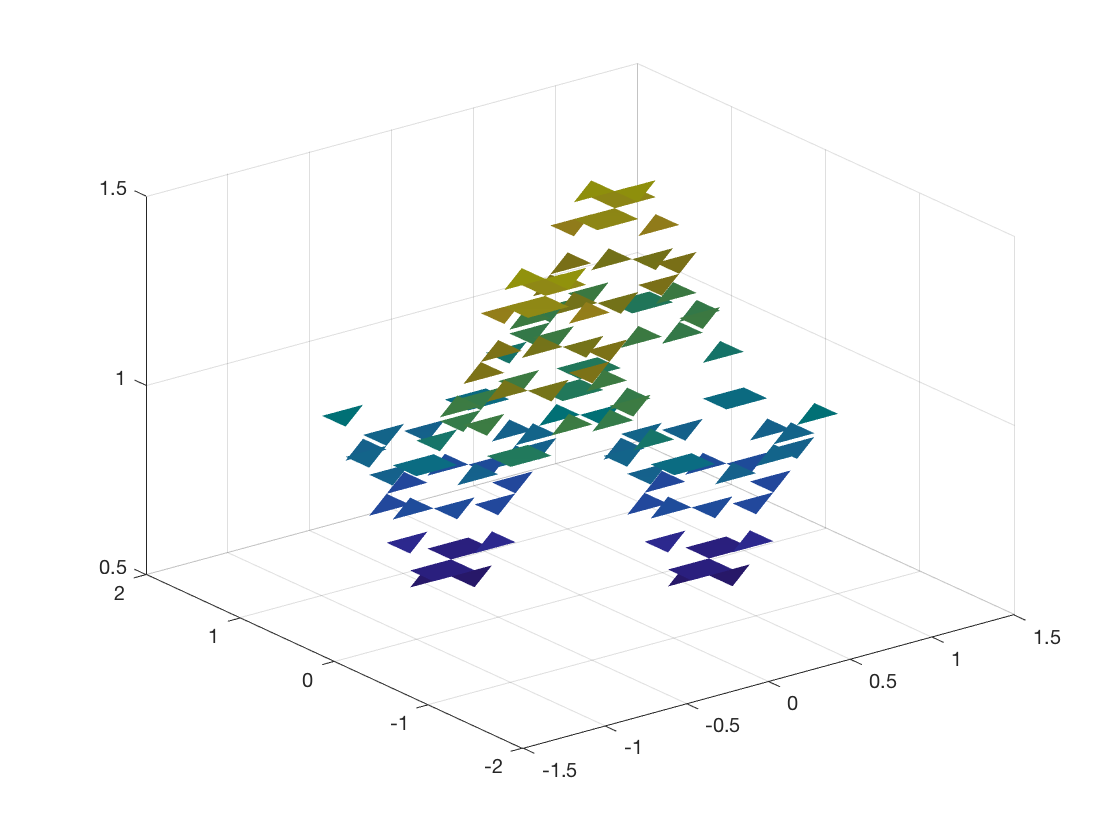
\includegraphics[width=.35\textwidth]{figs/cfun_M0.png}}
\hspace{-1em}
\subfloat[$M=1$ approximation]{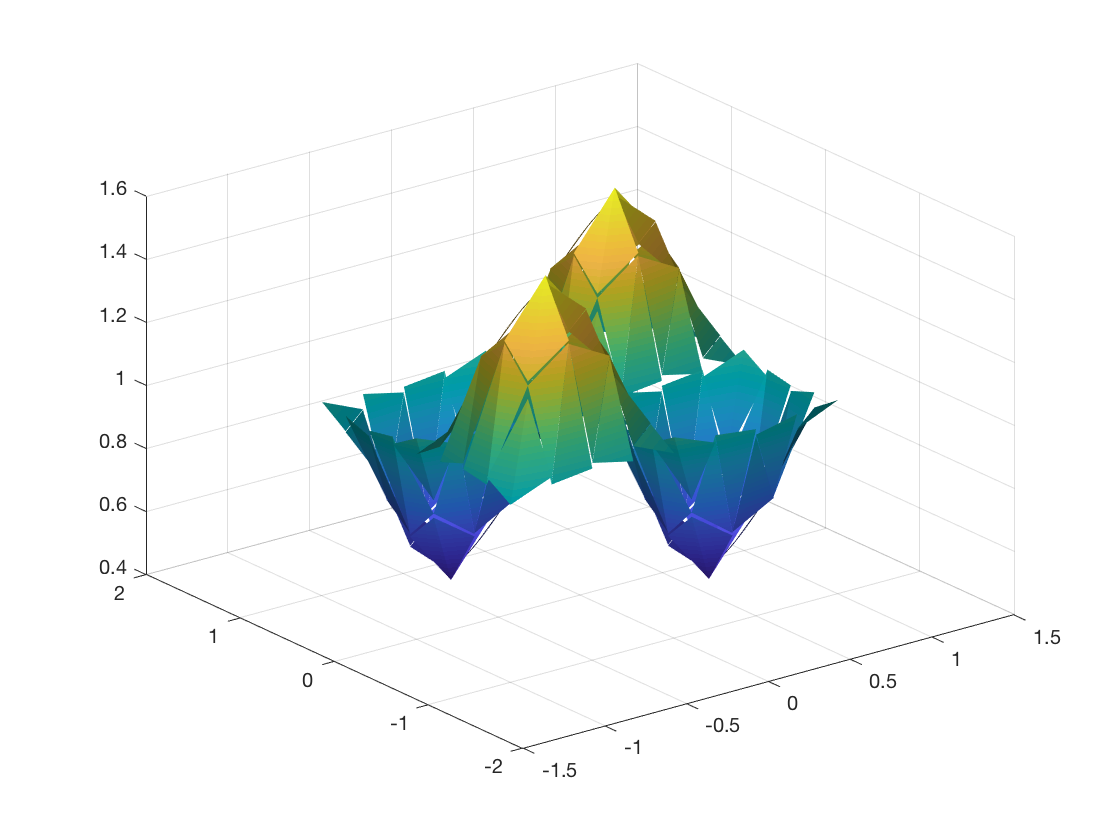
\includegraphics[width=.35\textwidth]{figs/cfun_M1.png}}
\end{figure}

\begin{itemize}
\item WADG reuses fast Bernstein volume and surface kernels.
\vspace{.5em}
%\item $O(N^6)$ update kernel: $\bm{V}_q$ interpolates $u(\bm{x})$ to quadrature points, scale by $c^2(\bm{x})$ at quadrature points, apply $\bm{P}_q$ to project back to $P^N$.
%\vspace{.5em}
%\item New approach: approx.\ $c^2(\bm{x})$ with degree $M$ polynomial, use fast Bernstein algorithms for polynomial multiplication and projection.
\item Fast $O(N^3)$ Bernstein algorithms for polynomial multiplication: represent $c^2 \in P^M$, $p(\bm{x}) \in P^{N}$, and construct $c^2(\bm{x})p(\bm{x})\in P^{M+N}$.
\vspace{.5em}
\item Fast $O(N^4)$ polynomial $L^2$ projection $\tilde{\bm{P}}_N: P^{M+N} \rightarrow P^N$.
\end{itemize}
}

%\frame[noframenumbering]{
%\frametitle{Quadrature-based WADG}
%
%}

%\frame[noframenumbering]{
%\frametitle{Sketch of Bernstein polynomial multiplication, projection}
%
%\only<1>{
%\begin{figure}
%\centering
%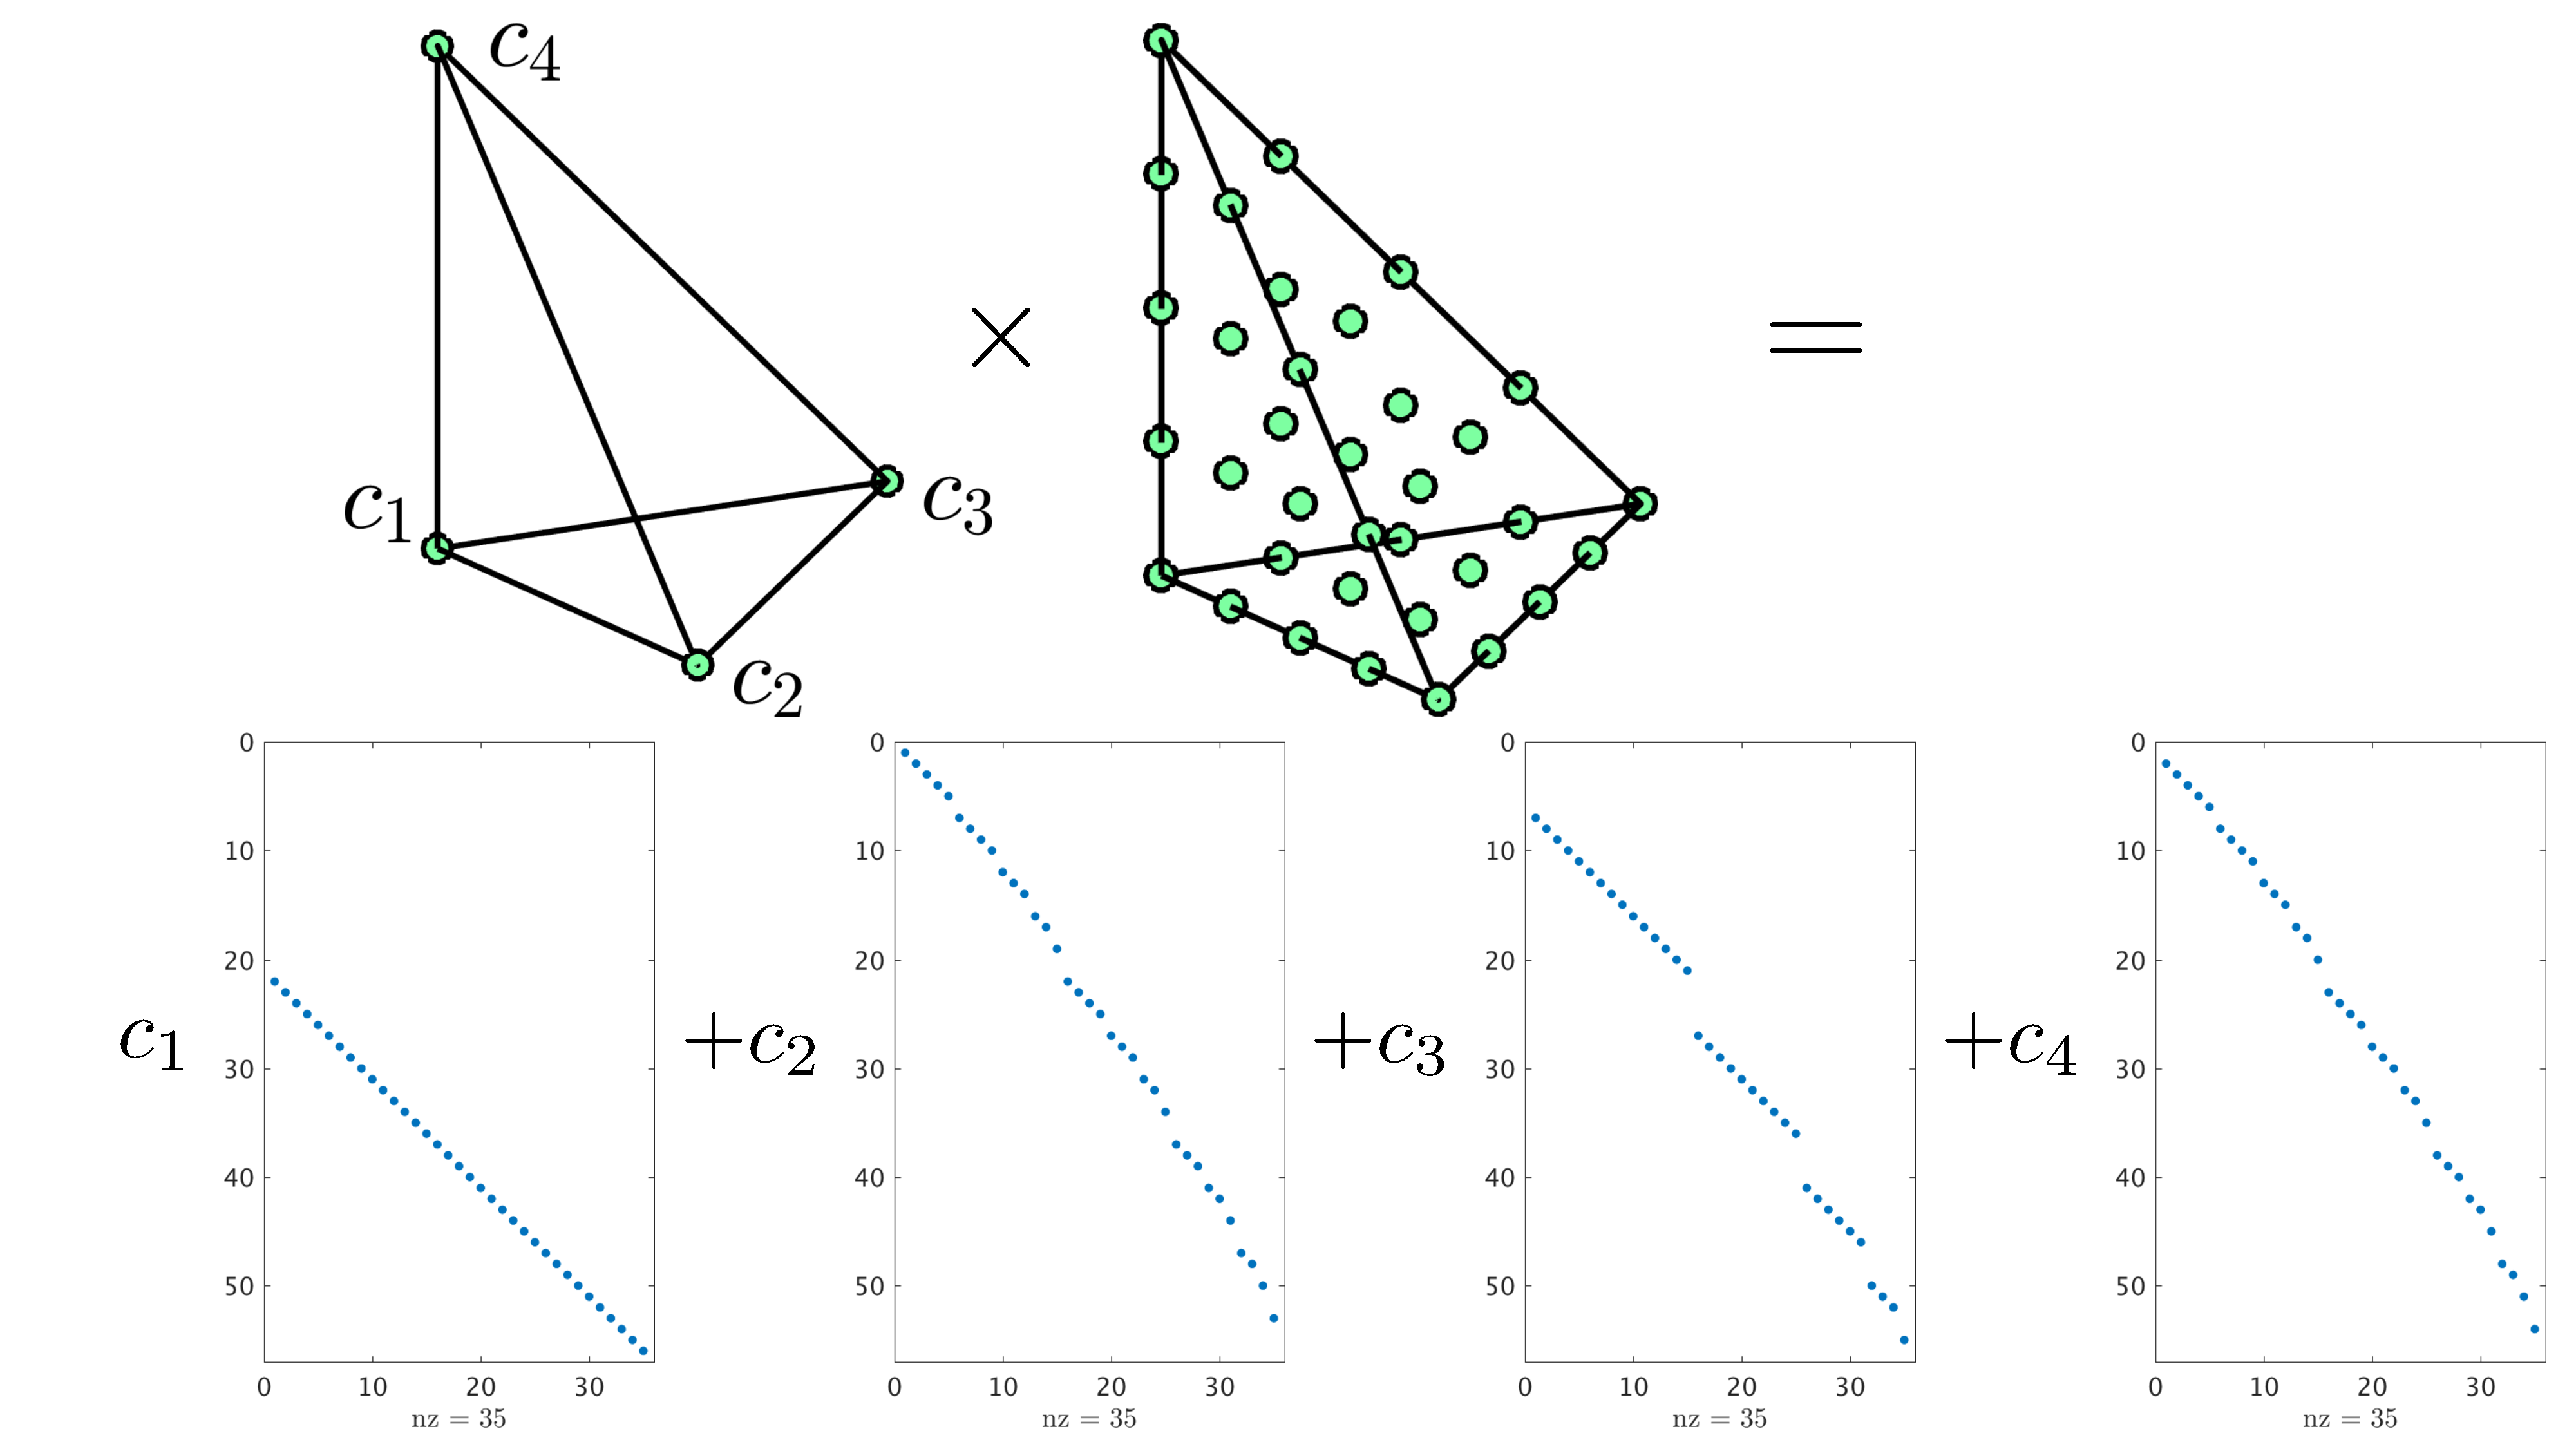
\includegraphics[width=.95\textwidth]{figs/polymult.pdf}
%\caption*{Bernstein polynomial multiplication: for fixed $M$, $O(N^3)$ complexity.}
%\end{figure}
%}
%\only<2>{
%\vspace{-.75em}
%\begin{figure}
%\centering
%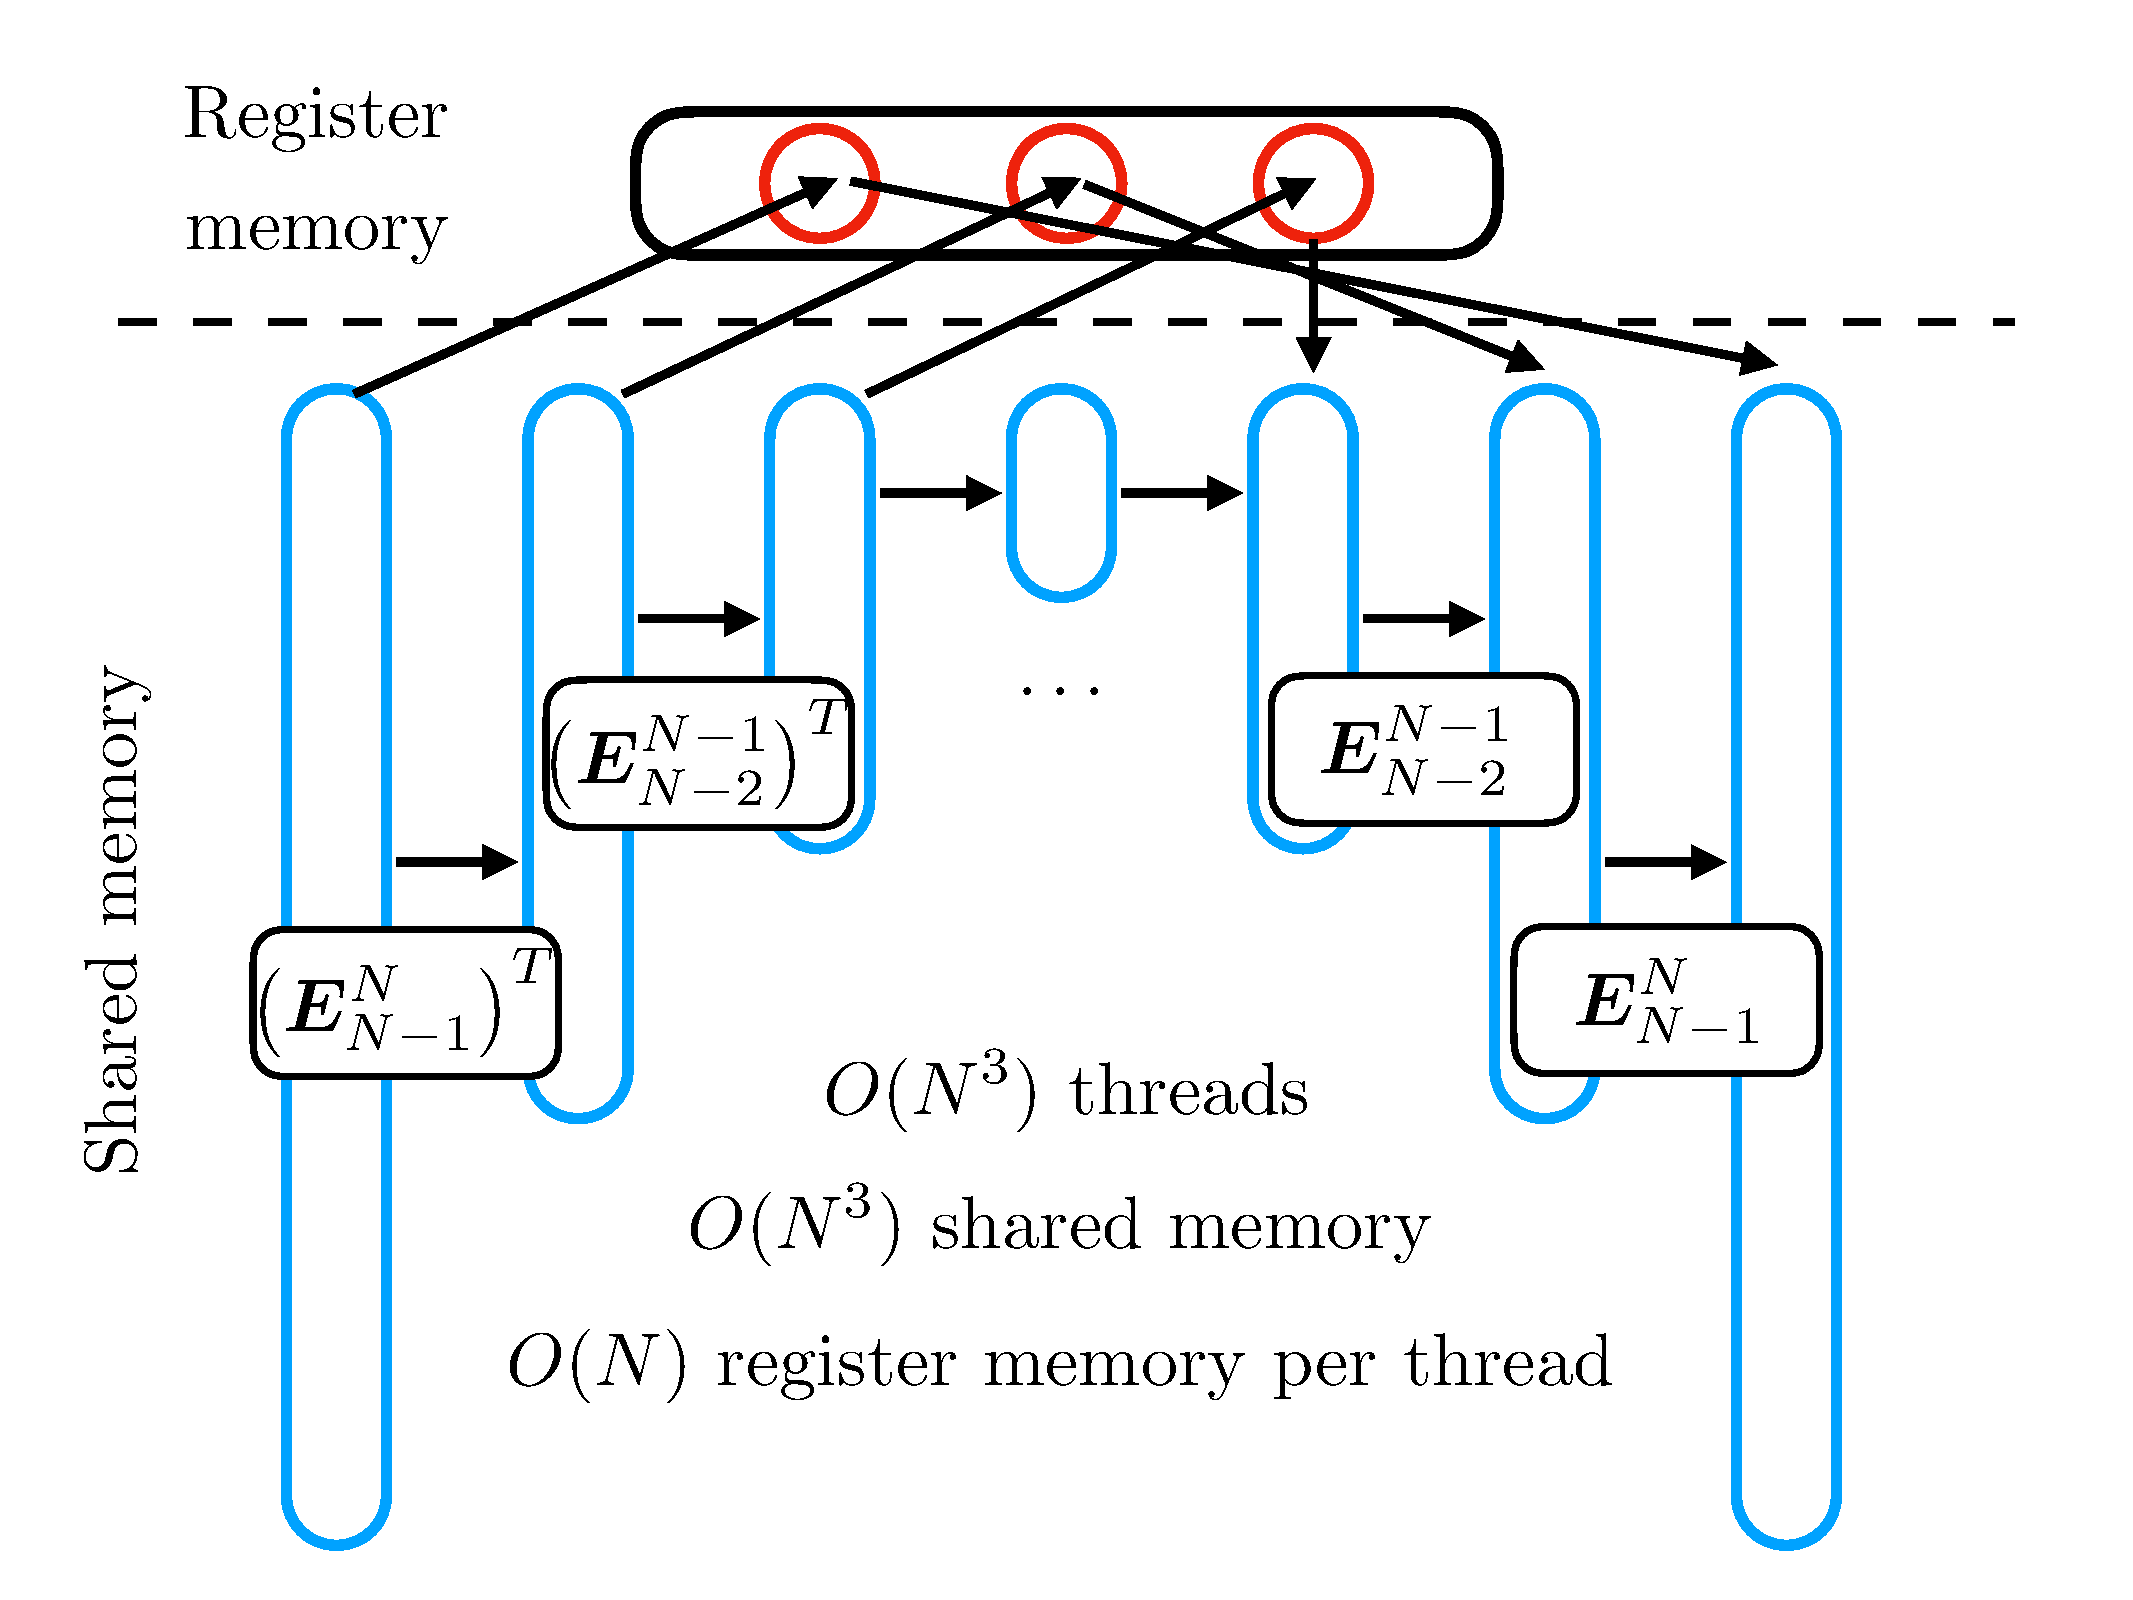
\includegraphics[width=.75\textwidth]{figs/bbproj.pdf}
%\end{figure}
%\vspace{-.5em}
%\[
%\tilde{\bm{P}}_N = \left(c_0\bm{I}+\bm{E}^N_{N-1}\left(c_1\bm{I}+\bm{E}^{N-1}_{N-2}\left(c_2\bm{I}+\cdots\right)\left(\bm{E}^{N-1}_{N-2}\right)^T\right)\left(\bm{E}^N_{N-1}\right)^T\right)
%\]
%}
%}

\frame[noframenumbering]{
\frametitle{BBWADG: computational runtime for $M=1$ }
\setcounter{subfigure}{0}
%\vspace{-.5em}
\begin{figure}
%\centering
\subfloat[]{
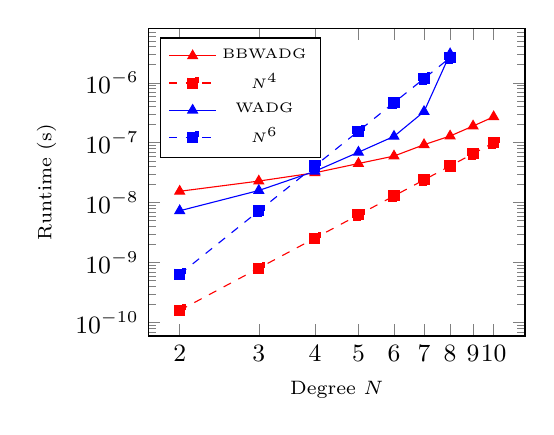
\begin{tikzpicture}
\begin{loglogaxis}[
width=.525\textwidth,
%title = {Update kernel  for $M=1$: runtime per element },
xlabel=Degree $N$,
ylabel=Runtime (s),
xtick = data,
ticklabel style = {font=\small},
xticklabels={$2$,$3$,$4$,$5$,$6$,$7$,$8$,$9$,$10$},
legend style={font=\tiny},
legend pos = north west
]
\addplot[color=red,mark=triangle*] 
coordinates {
	(2,0.0000000154975 )
	(3,0.0000000229375)
	(4,0.0000000315594)
	(5,0.0000000449963)
	(6,0.0000000599558)
	(7,0.0000000927645)
	(8,0.000000129382)
	(9,0.000000189771)
	(10,0.000000270587)
};

\addplot[dashed, color=red,mark=square*] coordinates {
	(2,0.00000000016)
	(3,0.00000000081)
	(4,0.00000000256)
	(5,0.00000000625)
	(6,0.00000001296)
	(7,0.00000002401)
	(8,0.00000004096)
	(9,0.00000006561)
	(10,0.00000010000)
};
\addplot[color=blue,mark=triangle*] 
coordinates{(2,7.33677e-09)(3,1.5973e-08)(4,3.3419e-08)(5,6.9422e-08)(6,1.27759e-07)(7,3.30517e-07)(8,3.03384e-06)};
%coordinates {
%	(2,0.0000000101731 )
%	(3,0.0000000199103)
%	(4,0.0000000368739)
%	(5,0.0000000822495)
%	(6,0.000000242786)
%	(7,0.00000046937)
%	(8,0.00000289899)
%};

\addplot[dashed, color=blue,mark=square*] coordinates {
	(2,0.00000000064)
	(3,0.00000000729)
	(4,0.00000004096)
	(5,0.00000015625)
	(6,0.00000046656)
	(7,0.00000117649)
	(8,0.00000262144)
};
\legend{BBWADG,$N^4$, WADG, $N^6$}
\end{loglogaxis}
\end{tikzpicture}
}
\hspace{-1em}
\subfloat[]{
	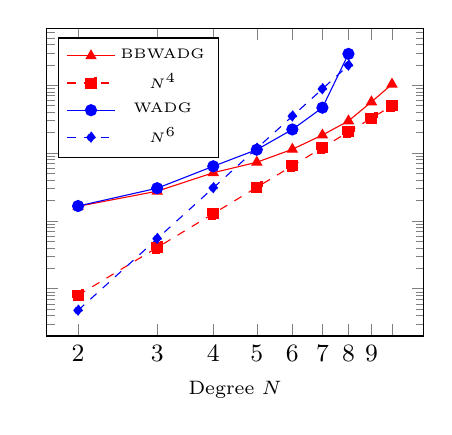
\begin{tikzpicture}
	\begin{loglogaxis}[
	width=0.525\textwidth,
	xlabel=Degree $N$,
%	ylabel=Runtime (s),
	xtick = data,
	ticklabel style = {font=\small},
	xticklabels={$2$,$3$,$4$,$5$,$6$,$7$,$8$,$9$},
	yticklabels={},
	legend style={font=\tiny},
	legend pos = north west
	]
	\addplot[color=red,mark=triangle*] coordinates {
		(2,0.0000000164062)
		(3,0.0000000274088)
		(4,0.0000000513347)
		(5,0.0000000732532)
		(6,0.000000113672)
		(7,0.000000184246)
		(8,0.000000297712)
		(9,0.000000567312)
	   (10,0.00000103571)
	};
	
	\addplot[dashed, color=red,mark=square*] coordinates {
		(2,0.00000000080)
		(3,0.00000000405)
		(4,0.00000001280)
		(5,0.00000003125)
		(6,0.00000006480)
		(7,0.00000012005)
		(8,0.00000020480)
		(9,0.00000032580)
		(10,0.00000050000)
	};
	
	
	\addplot[color=blue,mark=otimes*] coordinates {
		%(2,0.0000000101731 )
		(2,0.0000000165785)
		%(3,0.0000000199103)
		(3,0.0000000303376)
		%(4,0.0000000368739)
		(4,0.0000000638907)
		%(5,0.0000000822495)
		(5,0.000000112254)
		%(6,0.000000242786)
		(6,0.000000222803)
		%(7,0.00000046937)
		(7,0.000000466516)
		(8,0.00000289899)
	};
	
	\addplot[dashed, color=blue,mark=diamond*] coordinates {
		%(2,0.00000000064)
		%(3,0.00000000729)
		%(4,0.00000004096)
		%(5,0.00000015625)
		%(6,0.00000046656)
		%(7,0.00000117649)
		%(8,0.00000262144)
		(2,0.00000000048)
		(3,0.00000000547)
		(4,0.00000003072)
		(5,0.00000011719)
		(6,0.00000034992)
		(7,0.00000088237)
		(8,0.00000196608)
	};		
	\legend{BBWADG,$N^4$, WADG,$N^6$}
	\end{loglogaxis}
	\end{tikzpicture}
}
\end{figure}

}

\frame[noframenumbering]{
\setcounter{subfigure}{0}
\frametitle{BBWADG: update kernel speedup over WADG (acoustics)}

\begin{table}
   \centering
   \begin{tabular}{|c||c|c|c|c|c|c|c|} % Column formatting, @{} suppresses leading/trailing space
 \hline
%& $N=2$ 
& $N=3$ & $N=4$ & $N=5$ & $N=6$ & $N=7$ & \textcolor{red}{$N=8$} \\
   \hline
%WADG  &  1.86e-8 &  3.74e-8  & 8.08e-8  & 2.34e-7 &   4.68e-7 &  2.90e-6\\
WADG  &          1.60e-8  &  3.34e-8 &   6.94e-8 &  1.28e-7 &  3.31e-7  &  \textcolor{red}{3.03e-6}\\
  \hline
BBWADG &   2.20e-8 &  3.30e-8 &   4.42e-8 &   6.01e-8 &  9.46e-8 & 1.31e-7 \\
  \hline
%Speedup & 0.85 &  1.13 & 1.83  & 3.90 & 4.95 & 22.2\\
Speedup &    0.7260 &    1.0127 &    1.5706 &    2.1258 &    3.4938 &   \textcolor{red}{23.1591}\\
  \hline
\end{tabular}  
\vspace{.5em} 
\caption*{For $N\geq 8$, quadrature (and WADG) becomes much more expensive.}
\end{table}
\vspace{-2em}
\begin{figure}
\centering
\subfloat[$N= 7$ quadrature]{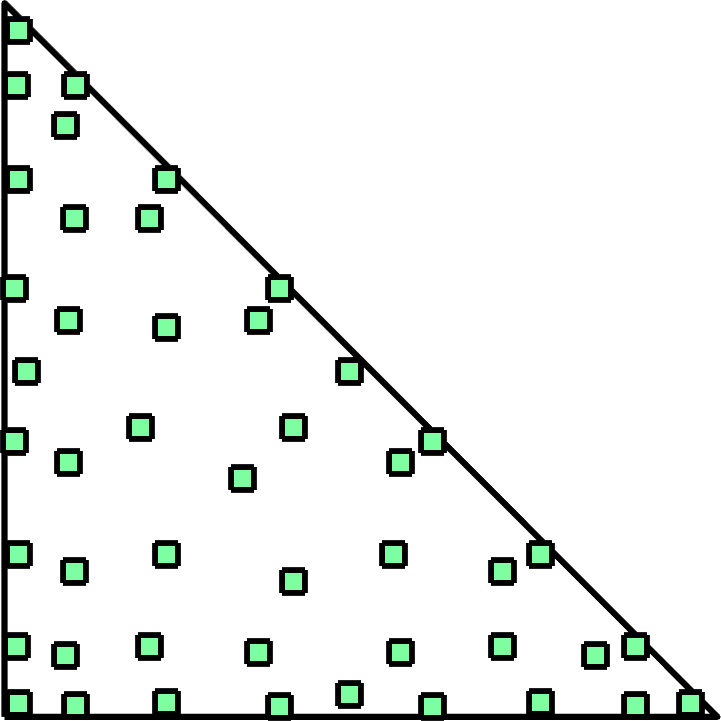
\includegraphics[width=.275\textwidth]{figs/quadrature_noTP.png}}
\hspace{2em}
\subfloat[$N =  8$ quadrature]{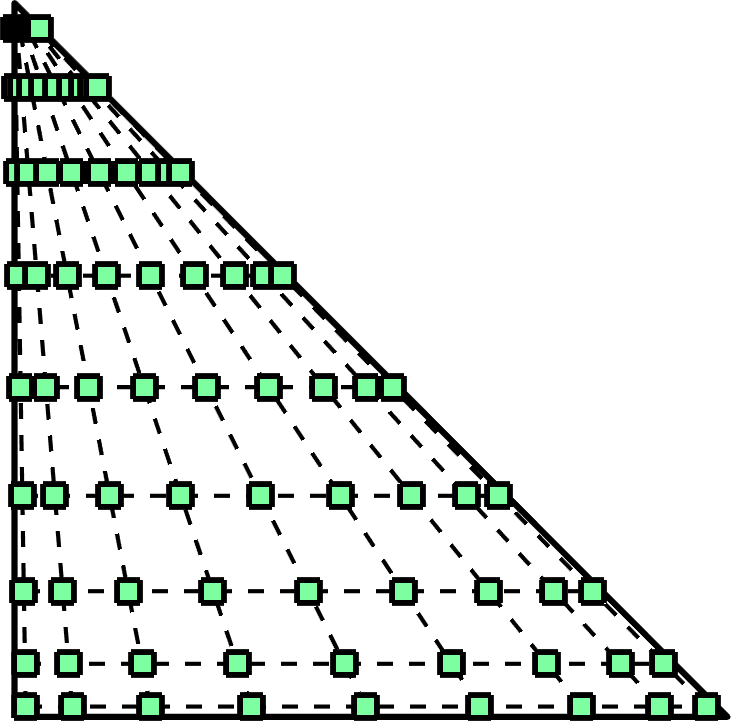
\includegraphics[width=.275\textwidth]{figs/quadrature_TP.png}}
%\caption*{For $N\geq 8$, WADG becomes much more expensive (more quadrature points).}
\end{figure}
}



\frame[noframenumbering]{
\frametitle{BBWADG: approximating $c^2$ and accuracy}

\begin{figure}
\centering
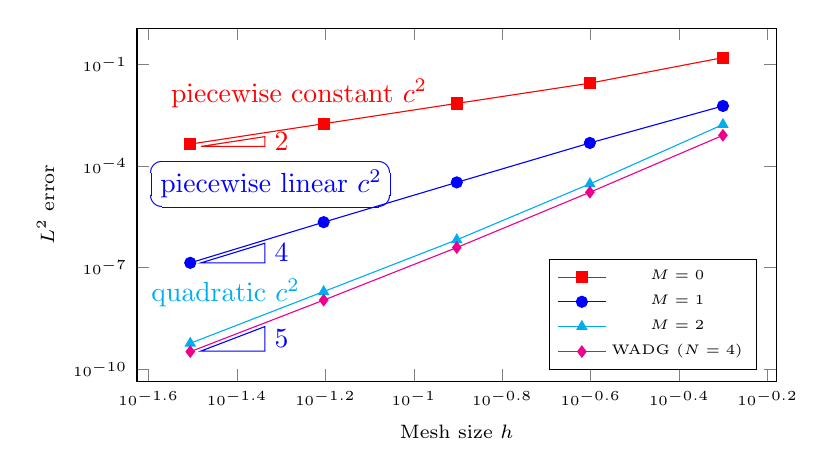
\begin{tikzpicture}
\begin{loglogaxis}[
width=0.8\textwidth,
height=0.5\textwidth,
title style = {font=\small},
%title = {Convergence of Bernstein-B\'ezier WADG ($N=4$)},
xlabel= Mesh size $h$,
ylabel= $L^2$ error,
ticklabel style = {font=\tiny},
%xtick = data,
%xticklabels={$2$,$3$,$4$,$5$,$6$,$7$,$8$},
%ymin=0.0000000001,ymax=1,
legend style={font=\tiny},
legend pos = south east
]
\addplot[color=red,mark=square*] coordinates {
	(0.5,0.1575135 )
	(0.25,0.02778378)
	(0.125,0.00701356)
	(0.0625,0.001763432)
	(0.0312,0.0004414745)
	};

%\addplot[color=blue,mark=otimes*] coordinates {
%	(0.5,0.05666667 )
%	(0.25,0.01566016)
%	(0.125,0.0007522236)
%	(0.0625,0.0000660265)
%	(0.0312,0.0000042542)
%	};

\addplot[color=blue,mark=otimes*] coordinates {
	(0.5,0.00590602 )
	(0.25,0.0004771556)
	(0.125,0.000032725844293)
	(0.0625,0.0000021917583)
	(0.0312,0.000000138034585)
	};

%\addplot[color=red,mark=triangle*] coordinates {
%	(0.5,0.03162 )
%	(0.25,0.054654)
%	(0.125,0.01402863)
%	(0.0625,0.00065991)
%	(0.0312,0.000058665)
%	};
\addplot[color=cyan,mark=triangle*] coordinates {
	(0.5,0.001672084 )
	(0.25,0.000029571618)
	(0.125,0.000000659821706)
	(0.0625,0.000000019551547)
	(0.0312,0.000000000582975)
	};
%\addplot[color=blue,mark=diamond*] coordinates {
%	(0.5,0.098363 )
%	(0.25,0.0331846)
%	(0.125,0.0541294)
%	(0.0625,0.01390139)
%	(0.0312,0.000656537)
%	};
\addplot[color=magenta,mark=diamond*] coordinates {
	(0.5,0.00080421 )
	(0.25,0.0000167281)
	(0.125,0.00000039029)
	(0.0625,0.0000000109402)
	(0.0312,0.000000000329775504)
	};

\logLogSlopeTriangle{0.2}{0.1}{0.085}{5}{blue};
\logLogSlopeTriangle{0.2}{0.1}{0.665}{2}{red};
\logLogSlopeTriangle{0.2}{0.1}{0.335}{4}{blue};
%\addplot[dashed, color=black,mark=diamond*] coordinates {
%	(0.5,3.1250000000000)
%	(0.25,0.09765625)
%	(0.125,0.0030517578)
%	(0.0625,0.00009536743)
%	(0.0312,0.000002956466553)
%	};

\node[above,red] at (axis cs: .055,.00275){piecewise constant $c^2$};
\node[above,blue] at (axis cs: .0475,.000003){\ovalbox{piecewise linear $c^2$}};
\node[above,cyan] at (axis cs: .0375,.0000000035){quadratic $c^2$};
\legend{$M=0$,$M=1$, $M=2$, WADG ($N=4$)}
\end{loglogaxis}
\end{tikzpicture}
%\caption*{Convergence of BBWADG for $M=0, 1,2$ and $N=4$.}
\end{figure}
\begin{center}
Approximating smooth $c^2(\bm{x})$ using $L^2$ projection:\\
\textcolor{red}{$O(h^2)$} for $M=0$, \textcolor{blue}{$O(h^{4})$} for $M = 1$, $O(h^{M+3})$ for $0 < M \leq N-2$. 
\end{center}
%\vspace{-.5em}
%\begin{itemize}
%\item Approximating smooth $c^2$ using $L^2$ projection: $O(h^2)$ for $M=0$, $O(h^{4})$ for $M = 1$.
%\item $O(h^{M+3})$ for $0 < M \leq N-2$. 
%%\item Interpolation: $O(h^{M+1})$ for $M$ odd, $O(h^{M+2})$ for $M$ even.
%\end{itemize}
}

\bibliographystyle{plain}
{\scriptsize
\bibliography{pyramids}
}

\end{document}
